\documentclass  [paper=a4,
				fontsize=12pt,
				listof=totoc,
				bibliography=totoc
				]{scrreprt}
\usepackage[T1]{fontenc}
\usepackage[utf8]{inputenc}
\usepackage{mathptmx}				%Font: Times New Roman
%\usepackage[default]{droidserif}	%Font: Droid Serif
\usepackage[ngerman]{babel}
%Seitenränder einstellen
\usepackage[head=2cm,bottom=2cm, left=25mm, right= 25mm ]{geometry}
%Paket für Erzeugung eines Abkürzungsverzeichnis, über das auch per Befehl im späteren Text auf diese verwiesen werden kann
\usepackage[printonlyused,smaller]{acronym}
%Paket zur Gestaltung der Kopf- und Fusszeile bei KOMA-Script
\usepackage{scrpage2}
\usepackage[hidelinks]{hyperref}
%Bibliograpie Packages / Settings
\usepackage{ragged2e} % Ermöglicht Flattersatz mit Silbentrennung
\usepackage[babel,german=guillemets]{csquotes}
% damit werden Zitate in französische Anführungszeichen gesetzt
\usepackage[%
backend=biber,% damit wird bestimmt, dass Sie mit der biber.exe arbeiten
bibencoding=utf8,% steht für die Kodierung der .bib-Datei
bibwarn=true,% damit werden ggf. enstandene Fehler ausgegeben
style=alphabetic,% hier wird die DIN 1505-T2 eingebunden
%firstinits=true% der Familienname des Authors wird an die erste Stelle
% gesetzt und anschließend der Vorname nur mit dem ersten
% Buchstaben abgekürzt ausgegeben
]{biblatex}
\usepackage[babel]{microtype} % bringt optischen Randausgleich und
% minimale Skalierung der Buchstaben
\setlength\bibitemsep{8pt} % Abstand zwischen 2 Einträgen im Verzeichnis
% nachfolgend wird der Kopf des Literaturverzeichnisses bestimmt
\defbibheading{online}{\subsection*{Online-Quellen}}
\defbibheading{offline}{\subsection*{Literatur}}
\ExecuteBibliographyOptions{
%isbn=false, % falls die ISBN hinterlegt ist wird diese ausgeblendet
}
\addbibresource{bibliothek.bib} % Einbindung der Literaturquelldatei
%Fortlaufende Fußnoten
\usepackage{chngcntr}
\counterwithout{footnote}{chapter}
%Paket zum Einbinden von Grafiken
\usepackage[pdftex]{graphicx}
\usepackage{wrapfig}
\usepackage{caption}


% Bibtexkey vor Quellenangabe (Jedoch nur bei stlye=alphabetic)
\DeclareFieldFormat{labelalpha}{\thefield{entrykey}}
\DeclareFieldFormat{extraalpha}{}

\usepackage{filecontents}
\usepackage{multicol}
\usepackage{relsize} %Einbinden der benötigten Pakete über die Datei Pakete.tex, wobei die Dateiendung weggelassen wird
\hyphenation{words} % LaTeX Wörter übergeben werden, die es entweder nicht selbstständig trennen kann(und hierdurch die entsprechenden Stellen markiert werden) oder nicht trennen soll\textbf{}
\counterwithout{figure}{chapter}
\counterwithout{table}{chapter} 
\begin{document}
	\parindent 0pt %entfernt den Einzug nach Absätzen
%	\pagestyle{empty} %\pagestyle{empty} sorgt dafür, das keine Seitenzahl auf der entsprechenden Seite auftaucht
	\begin{titlepage}
\begin{figure}
  \begin{center}
    \hbox to \hsize{%
      \begin{tabular}[m]{c}
        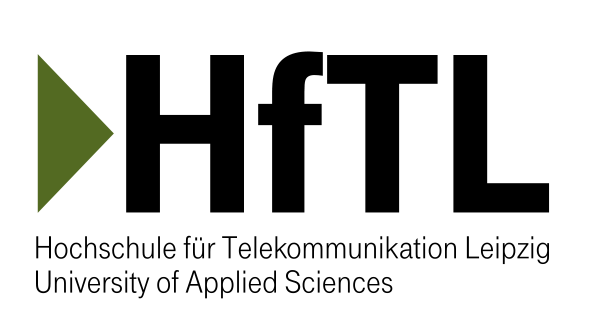
\includegraphics[width=2.5cm]{images/HfTL-Logo.png}
      \end{tabular}
      \hfill%
      \begin{tabular}[m]{c}
        Hochschule für Telekommunikation Leipzig (FH)\\
        Wirtschaftsinformatik \\
        Wissenschaftlich angeleitete Berufspraxis III\\
      \end{tabular}%
    }
  \end{center}
\end{figure}

\begin{center}
\rule{0pt}{0pt}
\vfill
\vfill
\vfill
\vfill

\begin{huge}
WAB III Projektarbeit:\\[0.75ex]
\dots\\[0.75ex]
E-Mail-Sicherheit\\[0.75ex]
\dots\\[0.75ex]
\end{huge}

\vfill
\vfill

Projektarbeit\\ von\\

\vspace*{.5cm}
Pascal Feller\\
Daniel Moy\\
Florian Schünhoff\\
Chi Cong Tran\\
\vspace{.5cm}
28. Juni 2014\\

\vfill
\vfill
\vfill
\vfill

\begin{tabular}{rl}
Referent, Betreuer:   & Prof. Dr. - Ing. Undine Pielot\\
\end{tabular}
\end{center}
\end{titlepage}



\newpage
\pagestyle{empty}


\text{ }
\vspace{11.5cm}




Hiermit versichern wir, dass wir die von uns vorgelegte Arbeit selbstständig verfasst haben, dass wir die verwendeten Quellen, Internet-Quellen und Hilfsmittel vollständig angegeben haben und dass wir die Stellen der Arbeit -- einschließlich Tabellen, Karten und Abbildungen~--, die anderen Werken oder dem Internet im Wortlaut oder dem Sinn nach entnommen sind, auf jeden Fall unter Angabe der Quelle als Entlehnung kenntlich gemacht haben.\\

Leipzig, den 28. Juni 2014\\
\medskip
\medskip

(Unterschrift)\\
\underline{~~~~~~~~~~~~~~~~~~~~~~~~~~~~~~~~~~~~~~~~}\\
Pascal Feller\\
\underline{~~~~~~~~~~~~~~~~~~~~~~~~~~~~~~~~~~~~~~~~}\\
Daniel Moy\\
\underline{~~~~~~~~~~~~~~~~~~~~~~~~~~~~~~~~~~~~~~~~}\\
Florian Schünhoff\\
\underline{~~~~~~~~~~~~~~~~~~~~~~~~~~~~~~~~~~~~~~~~}\\
Chi Cong Tran\\

\newpage


	\pagebreak	%Seitenumbruch
	\pagenumbering{Roman}
%\clearpage
%\begingroup
%  \renewcommand*{\chapterpagestyle}{empty}
  \pagestyle{plain}
\begin{small}
  \tableofcontents
%  \clearpage
%\endgroup	
	%\pagebreak
	\listoffigures %Abbildungsverzeichnis
	\pagebreak
	\listoftables %Tabellenverzeichnis
	\pagebreak
	\phantomsection \addcontentsline{toc}{chapter}{Abkürzungsverzeichnis}
\renewcommand\refname{Abkürzungsverzeichnis} \chapter*{Abkürzungsverzeichnis}
\begin{acronym}[StuRa] % In die optionale eckige Klammer die längste Abkürzung schreiben (für gemeinsame Ausrichtung)
	\acro{DHE}{Diffie-Hellmann-Verfahren}
	\acro{TLS/SSL}{Transport Layer Security/Secure Socket Layer}
	\acro{PFS}{Perfect Foreward Secrecy}
\end{acronym} %einbinden des in Akronyme.tex erstellten Abbildungsverzeichnisses
	\pagebreak
\end{small}
	\pagenumbering{arabic}\setcounter{page}{1} %ändern der Seitennummerierung auf arabische Zahlen und Beginn bei Seite 1
	% % % Kopf-und Fußzeilenumgebung / Einstellung % % %
		\pagestyle{fancyplain}
		\fancyhf{}							% http://www.sharelatex.com/learn/Headers_and_footers
		\renewcommand{\headrulewidth}{0.4pt}
		\footskip =30pt
		\renewcommand{\chaptermark}[1]{\markboth{#1}{}}	%"Kapitel 2." in Kopfzeile entfernen
		\rhead{\nouppercase{\leftmark}}	
		\lhead{E-Mail-Sicherheit}
		\lfoot{v1.0 \\ \today}
		\cfoot{\thepage\ / \pageref{LastPage}}
	% % % % % % % % % % % % % % % % % % % % % % % % % % %

\chapter{Einleitung}
		\section{Motivation}
		E-Mails werden in der Regel unverschlüsselt und im Klartext übertragen. Somit wird es Dritten ermöglicht, an den Inhalt dieser Mails zu gelangen. Nicht nur im geschäftlichen elektronischen Schriftverkehr ist es wichtig, dass ausgetauschte Nachrichten Dritten gegenüber unzugänglich gemacht werden. Im privaten Bereich ist es unter Umständen gewünscht oder gar erforderlich, dass die elektronische Kommunikation über E-Mails verschlüsselt wird, etwa bei vertraulichen Inhalten mit dem Arzt oder Behörden. Vielen Privatpersonen ist es mitunter unklar, welche Daten mitgelesen werden können. Zudem kennt nur eine geringe Anzahl der betroffenen Personen die verschiedenen Möglichkeiten zum Schutz bei der E-Mail-Kommunikation. Diese Thematik ist durch die jüngsten Enthüllen von Edward Snowden (Stand 2014) verstärkt in das Interesse der Öffentlichkeit gerückt und hat auch im privaten Umfeld die Menschen für eine gesicherte Kommunikation sensibilisiert.
		
		\section{Zielsetzung}
		Diese wissenschaftliche Arbeit setzt sich damit auseinander, welche Sicherheitsvorkehrungen eine private Person treffen kann, damit Dritten der Inhalt ihrer Mails verwahrt bleibt und damit der Empfänger sicherstellen kann, dass er die Mail vollständig und unverändert erhalten hat. Darüber hinaus wird die Funktionsweise dieser Maßnahmen erläutert. Ergänzend wird auf den Aspekt der Authentizität eingegangen, d. h. ob der Kommunikationspartner wirklich derjenige ist, für den er sich ausgibt. \\
		
	
		Ziel dieser wissenschaftlichen Arbeit ist die Untersuchung der verschiedenen Möglichkeiten zum Schutz der Daten in der E-Mail-Kommunikation sowie die Analyse ihrer Funktionsweise. Zudem werden gängige ausgewählte E-Mail-Provider anhand einer Nutzwertanalyse dahingehend untersucht, ob sie die Verfahren und Möglichkeiten hinsichtlich der Datensicherheit anwenden bzw. anbieten.
		
		\section{Aufbau der Arbeit}
		% \color{darkred}
		% Abgrenzung hinsichtlich wissenschaftlicher Methoden.
		% Z.B. bei Sicherheitsbedürfnissen tiefgreifende Analyse um diese festzulegen (vgl. Zielgruppenanalyse)
		% Bzw. In Anlehnung an...(Unternehmen) hervorheben
		% Was ist Sicherheitsniveau, Kategorie, Bedürfnis?
		% \color{black}
		
		In Bezug auf die Datensicherheit existieren vier verschiedene Aspekte, die unabhängig voneinander betrachtet werden können. Um ein gemeinsames Grundverständnis für die weitere Arbeit zu bekommen, werden diese Aspekte im nächsten kurz erläutert.
		
		Die von Privatpersonen versendeten Mails haben unterschiedliche Anforderungen an die Vertraulichkeit der Nachricht. Anhand dieser Anforderungen lassen sich Sicherheitsniveaus zuordnen, die in Kapitel \ref{chap:sicherheitsniveaus} analysiert werden.
		
		Nachdem ein Grundverständnis für die verschiedenen Aspekte in der Datensicherheit und die unterschiedlichen Sicherheitsniveaus aufgebaut wurde, werden im fünften Kapitel die Technologien und Verfahren zum Schutz der Daten in der E-Mail-Kommunikation untersucht. In diesem Kapitel werden die kryptographischen Grundlagen und die zwei wesentlichen Arten des Vertrauensmodell erläutert. Zudem werden verschiedene Verfahren und Protokolle für den Schlüsselaustausch und für die Verschlüsslung von Information und Transport. Das Kapitel schließt mit einer Betrachtung des 
		Namensdienstes DNS und seinen Sicherheit erhöhenden Erweiterungen ab.
		
		Im sechsten Kapitel werden ausgewählte Mail-Provider in der Praxis dahingehend untersucht, ob sie die in dieser Arbeit untersuchten Technologien und Verfahren einsetzen bzw. als Option anbieten. Aus dieser Analyse wird eine Nutzwertanalyse erstellt, die die Anforderungen der verschiedenen Sicherheitsniveaus anhand der vorgestellten Provider übersichtlich in tabellarischer Form darstellt.
		
		Das letzte Kapitel schließt die Arbeit thematisch mit einer Zusammenfassung und einem Ausblick über die gegenwärtigen und möglichen Entwicklungen ab.
		
		

	%Dies ist die Vorlage für die einzelnen Kapitel, die jeweils mit Chapter als Kapiteltitel starten
	\chapter{Datensicherheit Einmaleins}\label{sec:datensicherheit-einmaleins}
	Unter Datensicherheit wird der Schutz von Daten in den Aspekten Verfügbarkeit, Vertraulichkeit und Integrität verstanden.\footcite[Vgl.][]{BSI2014} Im Gegensatz dazu beschreibt Datenschutz den Schutz von und den vertrauensvollen Umgang mit persönlichen Daten. In der IT-Sicherheit wird zusätzlich des Aspekt der Authentizität berücksichtigt.\footcite[Vgl.][]{Berliner2014} In diesem Abschnitt werden diese Aspekte näher betrachtet, da diese für das Verständnis der vorgestellten Techniken in den späteren Kapitel notwendig sind.
	\chapter{Datensicherheit Einmaleins}
	Im Gegensatz zum Datenschutz, der den Schutz von und den vertrauensvollen Umgang mit persönlichen Daten thematisiert, wird unter Unter Datensicherheit der Schutz von Daten in den Aspekten Verfügbarkeit, Vertraulichkeit und Integrität verstanden \footcite[Vgl.][]{BSI2014}.  In der IT-Sicherheit wird zusätzlich der Aspekt der Authentizität berücksichtigt.\footcite[Vgl.][]{Berliner2014} In diesem Abschnitt werden diese Aspekte näher betrachtet, da diese für das Verständnis der vorgestellten Techniken im weiteren Verlauf der Arbeit notwendig sind.
	
	%mit \section{title} wird ein Unterkapitel der ersten Gliederungsebene überschrieben
	\paragraph{Verfügbarkeit}
	
	Unter Verfügbarkeit wird das Vorhandensein von Infrastruktur, Software, sämtliche IT-Dienstleistungen sowie -Funktionalitäten und Daten verstanden, so dass der Anwender bei Bedarf darauf zugreifen und diese nutzen kann. Um dies zu gewährleisten, muss verhindert werden, dass
	\begin{itemize}
	\item Daten verschwinden oder nicht zugreifbar sind, wenn sie gebraucht werden,
	\item Programme nicht funktionsbereit sind, wenn sie aufgerufen werden sollen,
	\item Hardware und sonstige notwendige Mittel nicht funktionsfähig oder gar verschwunden sind, wenn sie für die Verarbeitung benötigt wird. \footcite[Vgl.][]{Berliner2014}
	\end{itemize}
	
	\paragraph{Integrität}
	
	Unter der Integrität der Daten wird verstanden, dass die Daten bei der Übertragung nicht unbemerkt verändert werden können und folglich wie vom Absender vorgesehen übermittelt wurden. Bei diesem Aspekt geht es demzufolge um die Unversehrtheit der Nachricht.
	
	\paragraph{Vertraulichkeit}
	
	Unter Vertraulichkeit versteht man den Schutz der Nachricht vor unbefugtem Zugriff durch Dritte. Nur der vorgesehen Empfänger soll in der Lage sein, den Inhalt der Nachricht zu erfahren.
	
	\paragraph{Authentizität}
	
	Bei der Authentizität geht es um den Nachweis, dass die beteiligten Kommunikationspartner tatsächlich diejenigen sind, für die sie sich ausgeben.
	
	\chapter{Sicherheitsniveaus}\label{chap:sicherheitsniveaus}
		%Pascal: Wäre noch toll wenn wir hier nochmal sagen das wir eigtnlich nach einer Wissenschaftlichen Methode vorgehen müssten, also ähnlich wie bei der Festlegung der Zielgruppe. Nur das wir aus Zeitgründen eben Annahmen treffen. Aber einfach das wir hier sagen können, wenn wir Zeit hätten, hätten wir eine Umfrage gemacht und diese so und so gestaltet...
	
	
		In den nachfolgenden Kapiteln dieser Arbeit werden verschiedene Möglichkeiten der Verschlüsselung von E-Mail Kommunikation vorgestellt und jeweils passende Sicherheitsniveaus zugeordnet. %das eher so ein Einleitungs-Einsatz
		
		Dabei erfolgt diese Zuordnung mit dem Ziel, einen optimalen Ausgleich zwischen Notwendigkeit und Aufwand der Verschlüsselung von E-Mails zu erhalten.
		\medskip\\
		
		%, sodass der Nutzer nach der Ermittlung eines geeigneten Sicherheitsniveaus eine aus Sicht der Autoren geeignete Verschlüsselungsmethode ermitteln kann.
	
	
		%Das nachfolgende Kapitel geht auf verschiedene Sicherheitsbedürfnisse eines Nutzers ein. 
		
		Gerade im Hinblick auf den Grad der Verschlüsselung bei der E-Mail Kommunikation ist es wichtig sich darüber bewusst zu werden, wie sensibel die Information ist, die man versenden möchte. Denn jede Verschlüsselung ist mit einem bestimmten Aufwand verbunden und folglich ist abzuwägen, welcher Verschlüsselungsaufwand dem Nutzer die zu versendende Information wert ist. 
		\medskip\\
		
		%Beispielsweise ist aus Sicht der Autoren der potentielle Schaden gering, wenn eine E-Card zu den Weihnachtsfeiertagen an den nicht rechtmäßigen Empfänger gerät, sodass für die Versendung einer solchen Information der Grad der Verschlüsselung niedrig und somit der Aufwand niedrig ausfällt. Dahingegen ist der potentielle Schaden größer, wenn es sich bei der versendeten Information um beispielsweise die eigenen Kontodaten handelt, was wiederum bedeutet, dass der Nutzer bereit ist einen höheren Aufwand zu betreiben, um diese Inhalte auf eine sichere Art und Weise via E-Mail zu übermitteln.
	
	
		%Das Sicherheitsbedürfnis einer jeden Person kann unterschiedlich stark ausgeprägt sein. 
		Der Wert einer Information ist durch das eigene Sicherheitsbedürfnis geprägt, welches jedoch von Person zu Person in unterschiedlicher Form ausgeprägt ist.
		
		Daher ist es den Autoren nicht möglich, eine allgemein gültige Auflistung aller möglichen Szenarien der E-Mail Kommunikation bereitzustellen, aus welcher die Teilnehmer der Zielgruppe lediglich das richtige Szenario heraussuchen müssen und dadurch den optimalen Grad der Verschlüsselung erhalten. 
		
		Stattdessen wird in Tabelle \ref{tab:sicherheitsniveaus} eine Übersicht präsentiert, die es dem Nutzer erlaubt auf Basis seines eigenen Sicherheitsbedürfnisses und mit Hilfe festgelegter Kriterien für die Übermittlung einer ganz bestimmten Information ein geeignetes Sicherheitsniveau zu bestimmen. 
		\medskip\\
		
		
		%In den nachfolgenden Kapiteln dieser Arbeit werden verschiedene Möglichkeiten der Verschlüsselung von E-Mail Kommunikation vorgestellt und jeweils passenden Sicherheitsniveaus zugeordnet. %das eher so ein Einleitungs-Einsatz
		%Dabei erfolgt diese Zuordnung mit dem Ziel, einen optimalen Ausgleich zwischen Notwendigkeit und Aufwand der Verschlüsselung von E-Mails zu erhalten, sodass der Nutzer nach der Ermittlung eines geeigneten Sicherheitsniveaus eine aus Sicht der Autoren geeignete Verschlüsselungsmethode ermitteln kann.
	
		%Wäre nice wenn die Abbildung eine Tabelle ist, weil eine Abbildung für eine Tabelle ist irgendwie komisch :D (Pascal)
		%Auch viel Sicht der Autoren, ich würde das zur Einleitung einmal allgmein sagen statt hier 3 Mal im Absatz. So bei der Abgrenzung / Zielsetzung / einleitung. Generell ein sehr Einleitungslastiger Abschnitt.
		
		Die Tabelle \ref{tab:sicherheitsniveaus} stellt im Tabellenkopf vier verschiedene Sicherheitsniveaus dar: \textit{Streng Vertraulich, Vertraulich, Privat und Öffentlich}. Dabei nimmt das Sicherheitsbedürfnis sowie der Verschlüsselungsaufwand von Streng Vertraulich bis Öffentlich ab.
		
		In der ersten Spalte sind verschiedene Merkmale aufgelistet, welche es dem Nutzer ermöglichen sollen, 
		%für eine ganz bestimmte Information 
		ein geeignetes Sicherheitsniveau zu bestimmen.
		%Nummern wären Klasse (Stufe 1-4)
		Alle weiteren Felder enthalten die Ausprägung des Merkmals innerhalb des jeweiligen Sicherheitsniveaus.
		\medskip\\
		
	\pagebreak
%	\begin{figure}[h] %{wrapfigure}[36]{l}{1.0\textwidth}
%			%\begin{center}
%		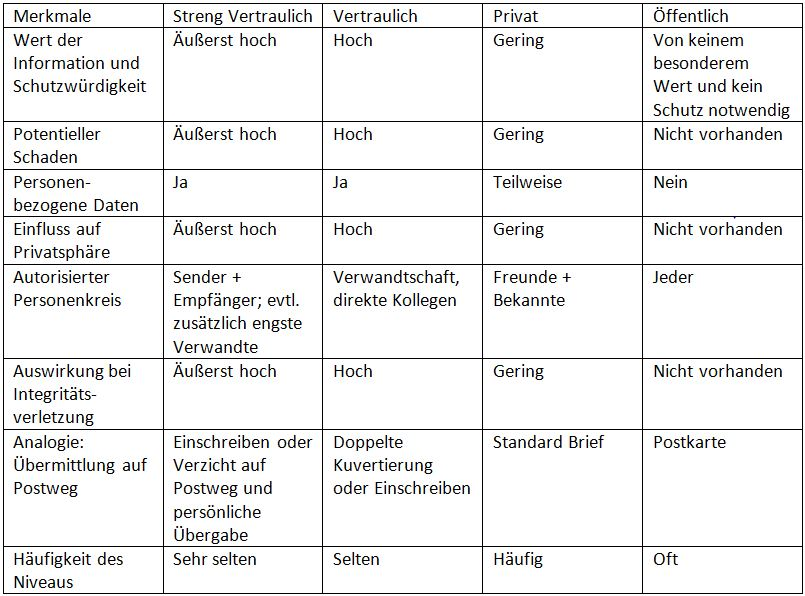
\includegraphics[width=16cm]{images/sicherheitsniveaus.jpg}
%			%\end{center}
%		\caption {Sicherheitsniveaus} %Bildunterschrift, erstes Argument ist für Abbildungsverzeichnis ohne Fußnote; \footnotemark ist ein Platzhalter für die Fußnote
%		\label{img:sicherheitsniveaus} %für Bezüge auf diese Abbildung
%	\end{figure} %wrapfigure}

	\begin{table}
		\small
		\centering
		\begin{tabularx}{\textwidth}{|>{\raggedright\arraybackslash}X|>{\raggedright\arraybackslash}X|>{\raggedright\arraybackslash}X|>{\raggedright\arraybackslash}X|>{\raggedright\arraybackslash}X|} 
			\hline Stufe & \multicolumn{1}{c|}{\textbf{4}} & \multicolumn{1}{c|}{\textbf{3}} & \multicolumn{1}{c|}{\textbf{2}} & \multicolumn{1}{c|}{\textbf{1}} \\
			  & \multicolumn{1}{c|}{\textbf{Streng Vertraulich}} & \multicolumn{1}{c|}{\textbf{Vertraulich}} & \multicolumn{1}{c|}{\textbf{Privat}} & \multicolumn{1}{c|}{\textbf{Öffentlich}} \\ 
			\hline Wert der Information, Schutzwürdigkeit & Äußerst hoch & Hoch & Gering & kein hoher Wert; kein Schutz notwendig \\ 
			\hline Personenbezogene Daten & Ja & Ja & Teilweise & Nein \\ 
			\hline Einfluss auf Privatsphäre & Äußerst hoch & Hoch & Gering & Nicht vorhanden \\ 
			\hline Autorisierter Personenkreis & Sender + Empfänger; evtl. zusätzlich engste Verwandte & Verwandtschaft & Freunde + Bekannte & Jeder \\ 
			\hline Auswirkung bei Integritätsverletzung & Äußerst hoch & Hoch & Gering & Nicht vorhanden \\
			\hline Analogie: Übermittlung Postweg & Einschreiben oder Verzicht auf Postweg und persönliche Übergabe & Doppelte Kuvertierung oder Einschreiben & Standard Brief & Postkarte \\
			\hline Häufigkeit des Niveaus & Sehr selten & Selten & Häufig & Oft \\  
			\hline
		\end{tabularx} 
		\caption{Sicherheitsniveaus}
		\label{tab:sicherheitsniveaus}
	\end{table}
		
		Der Wert der Information und deren Schutzwürdigkeit beschreiben, wie wertvoll die zu versendende E-Mail für einen nicht rechtmäßigen Empfänger ist und welche Notwendigkeit des Schutzes daraus folgt.
		
		Der potentielle Schaden stellt das Ausmaß dar, welches eintritt für den Fall, dass die E-Mail durch 
		%unberechtigte 
		Dritte (klassische Angreifer sowie der E-Mail Provider) gelesen wird. Dieser Schaden kann verschiedener Art sein. Zum Beispiel können daraus rechtliche Konsequenzen erfolgen, es kann zu einem finanziellen Verlust führen oder mit einer Schädigung des Images des Senders einhergehen.\footcite[Vgl.][S. 6]{ReinhausenGmbH} Aus dem potentiellen Schaden lässt sich außerdem gut der Einfluss auf die eigene Privatsphäre ableiten.
		
		
		%Habe aus Einzahl mal mehrzahl gemacht. Unberechtigte Dritte ist schwierig weil der Mailprovider ist ja quasi Berechtigt, jedenfalls stellt er das (glaub ich) zumindest in den AGBs klar. Würde nur "Dritte" sagen oder? Dazu müsste man noch klarstellen wer Dritte sind, oder verweisen (Klassische Angreifer oder Provider, Bots)
		Das Merkmal \textit{Personenbezogene Daten} besagt, dass die zu versendende Information personenbezogene Daten enthält und daher grundsätzlich das Sicherheitsniveau \textit{Vertraulich} zu wählen ist.\footcite[Vgl.][]{TSE} In Abhängigkeit von der Ausprägung der anderen Merkmale, kann als resultierendes Sicherheitsniveau auch \textit{Streng Vertraulich} oder \textit{Privat} ermittelt werden.
		
		
		%Evtl die Beschreibungen mehr gleidern, in Absätzen oder Bullets? Weil so mitten im Text ist allg. der Text so als "Batzen" schwer zu lesen, und man kann sich auch nicht eben man die Beschreibung zur Tabelle 'heraussuchen'
		Der Autorisierte Personenkreis ist eine weitere Eigenschaft anhand derer der Nutzer ein passendes Sicherheitsniveau bestimmen kann. Grundsätzlich gilt: je wertvoller die Information, desto geringer ist der Personenkreis, der Einblick in die zu versendende E-Mail erhalten darf.\footcite[Vgl.][]{TSE} Daraus folgt, dass eine streng vertrauliche Nachricht ausschließlich zwischen dem Sender und dem Empfänger ausgetauscht wird und in der Regel keine weitere Person über den Inhalt erfahren darf. Eine Ausnahme an dieser Stelle sind allenfalls engste Verwandte. Dahingegen ist für eine Nachricht, deren Inhalt prinzipiell jedermann erfahren darf, das Sicherheitsniveau \textit{Öffentlich} zu wählen.\footcite[Vgl.][S. 10]{ReinhausenGmbH}
		
		
		%Nachfolgend: Hier ist eindeutig ein Cut, aber deutlicher würde ich mir wünschen, eine section o.ä. wäre doch fast angebracht wenn jetzt die Auswirkungen kommen
		Die \textit{Auswirkung bei Integritätsverletzung} beschreibt das eingetretene Ausmaß, wenn die E-Mail in die Hände eines Angreifers gelangt ist.
		
		
		Eine weitere Möglichkeit ein geeignetes Sicherheitsniveau zu ermitteln ist die Überlegung, wie der Inhalt der E-Mail auf dem Postweg versandt werden würde. Für eine streng vertrauliche Information würde ein Einschreiben gewählt werden oder gänzlich auf den Postweg verzichtet und stattdessen die Nachricht persönlich überbracht werden. Dahingegen ist für Information, die ohne Bedenken  auf einer Postkarte übermittelt werden können, das Sicherheitsniveau \textit{Öffentlich} zu wählen 
		
		
		Das letzte Merkmal beschreibt das Aufkommen der einzelnen Sicherheitsniveaus. Streng vertrauliche Informationen sind sehr selten und am häufigsten werden öffentliche Nachrichten ausgetauscht.\footcite[Vgl.][]{TSE}
		\medskip\\
	%Auch wieder Cut Bsp: Anwenwedungsfälle als Section? dann Stufe 1-4 und die Fälle dazu? Das ist jetzt ein riesen Case, der unheimnlich kreativ ist und toll beschrieben. Eventuell kann es für ne wissenschaftl. Arbeit auch weniger sein nach dem Motto "Versicherungsschaden am Wagen. Bilder und Kontodaten per E-Mail an Versicherung senden: Streng vertraulich" Sowas hätte mir persönlich gereicht, und dazu vll noch ein Beispiel wie das mit den Patientendaten mit Röntgenbildern (auch streng vertraulich). Und zusätzlich noch ein paar cases zu den unteren stufen. Weihnachtsbild für die Familie mit Gesichtern : Vertraulich. Weihnachts E-Card von Webseite ohne Gesichter Öffentlich. Irgendwie sowas. Das soltlen wir besprechen am Freitag
	
		Anhand des nachfolgenden Beispiels soll der Umgang mit der Tabelle \ref{tab:sicherheitsniveaus} verdeutlicht werden. Hierbei ist zu erwähnen, dass das resultierende Sicherheitsniveau auf Basis des beschriebenen Sicherheitsbedürfnisses ermittelt wurde und für die gleiche Information bei anderen Nutzern unterschiedlich ausfallen kann:
		\medskip\\
		
		Herr Meier war vor kurzem in einen Auffahrunfall verwickelt, den ein unachtsamer Autofahrer verursacht hatte. Daraufhin brachte Herr Meier sein Fahrzeug in die Werkstatt und ließ ein Gutachten des Schadens erstellen. Dieses Gutachten möchte er nun zusammen mit seinen Kontodaten via E-Mail an die Versicherung des Unfallverursachers senden. 
		
		Der Wert dieser Information ist hoch, denn einerseits sind die Kontodaten in der Nachricht vorhanden. Andererseits ist in dem Gutachten Herr Meiers Anschrift angegeben und es lässt sich aus den Fotos und der Schadenshöhe des Gutachtens ableiten, dass Herr Meier einen Luxuswagen besitzt. Daraus wiederum lassen Rückschlüsse auf seine finanzielle Situation schließen. Der potentielle Schaden, der sich daraus ergibt, ist hoch bis äußerst hoch. Denn bei ausreichender krimineller Energie können nicht nur die Kontodaten missbraucht werden, sondern mit Hilfe der Anschrift kann der Wohnsitz von Herrn Meier ausgekundschaftet und beispielsweise bei seiner Abwesenheit in sein Anwesen eingebrochen werden. 
		
		Die Anschrift stellt personenbezogene Daten dar und ermöglicht einen hohen Einfluss auf die Privatsphäre von Herrn Meier.
		Der Autorisierte Personenkreis für diese Nachricht beschränkt sich auf den Sender (Herr Meier), den Empfänger (die Versicherung) sowie auf seine Frau und auf die Werkstatt, die das Gutachten erstellt hat. Seinen Freunden und Kollegen hat Herr Meier zwar auch von dem Unfall erzählt. Allerdings wissen diese keine genaueren Details hinsichtlich des Schadens und dessen Höhe.
		
		Hätte die Versicherung den E-Mail Service nicht angegeben, so würde Herr Meier die Unterlagen des Gutachtens mit einem Standard-Brief versenden. Die Kontodaten würde er mittels Einschreiben verschicken.
		\medskip\\
		
		Somit kann als Resultat für dieses Beispiel unter dem beschriebenen Sicherheitsbedürfnis ein Sicherheitsniveau von \textit{Vertraulich} ermittelt werden. Welches Verschlüsselungsverfahren konkret für dieses Sicherheitsniveau anzuwenden ist, wird in den nachfolgenden Kapiteln beschrieben.
		
%	\chapter{Gefahren und Schwachstellen}
%		\label{chap:gefahren}
%\color{darkred}
%		\section{Informationsgewinnung durch Provider}
%\textsl{
%warum ist E-Mail oft Kostenlos?\\
%Welchen Sinn hat das für die Provider?\\
%Welche Bots lassen die Provider über unsere Kommunikation laufen?\\
%Wie mächtig sind Meta-Daten?\\
%\\
%\\
%Überleitung... Neben den weniger gerichteten (Kein Angriff?) Maßnahmen der Informationsgewinnung aus E-Mail-Kommunikation gibt es auch klassische Angriffsmethoden Dritter.\\
%\\
%Internetquellen, die durch Literatur idealerweise belegt wird:\\
%\begin{itemize}
%\item \href{http://www.netzdurchblick.de/emails.html}{netzdurchblick.de}
%\item \href{https://www.eleven.de/aktuelle-pressemitteilungen.428/items/eleven-warnt-die-5-groessten-gefahren-fuer-e-mail-nutzer.html}{eleven.de}
%\item \href{https://www.bsi-fuer-buerger.de/BSIFB/DE/SicherheitImNetz/OnlineBanking/GefahrenUndSicherheitsrisiken/gefahren_sicherheitsrisiken_node.html}{BSI}
%\end{itemize}
%Diese Quellen dienen auch zur Übersicht. Belegt werden sollten diese noch durch Literatur, die ggf. zu suchen ist!}
%		 
%		\section{Angriffsarten}
%			\subsection{MITM - Man in the Middle}
%			\label{sec:mitm}
%\color{black}
%			\subsection{Umleitungsangriffe}
%			\label{sec:cache_poison}
%			Umleitungsangriffe werden mit dem sogenannten \ac{DNS} Cache Poisoning durchgeführt.
%			Bei diesem Angriff wird sich die Schwachstelle zu nutze gemacht, dass ältere oder falsch konfigurierte \ac{DNS}-Server auch nicht angeforderte Records in ihren Cache schreiben.
%			Ein Angreifer kann dies dazu nutzen im Cache eines \ac{DNS}-Servers mithilfe von gefälschten Paketen falsche Zuordnungen von Domainnamen zu \ac{IP}-Adressen zu hinterlegen.
%			Ein Opfer, das die Auflösung des Domainnamens jetzt vom kompromittierten Server anfordert, wird auf den Server des Angreifers umgeleitet.
%\color{darkred}
%			\subsection{Drive-By-Angriffe}
%\textsl{(eleven.de)}
%			\subsection{Phishing}
%\textsl{Auch Spear Phising (eleven.de)}
%			\subsection{Malware-E-Mails}
%\textsl{Auch: Lokalisierte Angriffe (eleven.de)}
%			\subsection{Spam}
%\textsl{Auch: Event-Spam (eleven.de)}
%
%		\section{Schwachstellen}
%			\subsection{Zertifikatsaussteller}
%			\label{sec:zertifikatsaussteller}
%\textsl{AUTHENTIZITÄT (DANE-Artikel)
%200 Aussteller (z.T. keine eigenen Private Keys der User) CAs können nachlässig werden. Angreifern können somit gültiges Zertifikat für einen Host erstellen dessen Besucher das Ziel sind.}
%			\subsection{Zertifikatsprüfung}
%			\label{sec:zertifikatspruefung}
%\textsl{AUTHENTIZITÄT (DANE-Artikel)
%Ideal wäre: Alle Serverzertifikate der gesamten Komunikationskette zu prüfen. In der Praxis jedoch kein sog. "Identifiziertes TLS" (Kommunikationspartner eindeutig festgestellt) In der Praxis arbeiten Server jedoch nach "Opportunistischem TLS", dass bedeutet das lediglich wichtig ist, dass die Nachricht verschlüsselt übertragen wird, egal von wem.}
%			\subsection{Metadaten}
%			\label{sec:metadaten}
%\textsl{Quellen:
%\href{http://www.spiegel.de/netzwelt/netzpolitik/google-urteil-eugh-entscheidung-zu-suchmaschinen-a-969302.html}{google-urteil-eugh-entscheidung-zu-suchmaschinen} \\
%\href{http://www.golem.de/news/stanford-experiment-metadaten-verraten-intimste-details-des-privatlebens-1403-105253.html}{metadaten-verraten-intimste-details-des-privatlebens}\\
%\href{http://www.heise.de/ct/heft/2014-4-Die-Schwaechen-der-E-Mail-und-was-dagegen-hilft-2092851.html}{Schwaechen-der-E-Mail-und-was-dagegen-hilft}}
%\color{black}
	
	\chapter{Technologien und Verfahren}
		\section{Kyptographie Grundlagen}
				Die Kryptographie ist die Wissenschaftslehre, die sich mit den Verfahren sowie der Anwendung von Ver- und Entschlüsselung von Informationen befasst. Dabei bedient sie sich mathematischen Hilfsmitteln, um die Daten vor Dritten unzugänglich zu machen. In diesem Kapitel werden zunächst die grundlegende Funktionsweise der Verschlüsselung untersucht, die zum Verständnis der weiteren Kapitel notwendig sind. Anschließend werden verschiedene Verfahren beleuchtet, die eine verschlüsselte und geschützte Kommunikation ermöglichen.
				%Die Einleitung ist top, mehr Bezug zur E-Mail wäre toll, so das es essenziel für Sicherheit ist und die Basis zur Sicherstellung von sicherer Kommunikation Stufe 1-4 (Unsere niveaus) da nämlich auch öffentlich zumindest transport verschlüsselt sein sollte (wird ja auch als Standard durchgedrück (versucht) EmiG, TLS)
			\subsection{Symmetrische Verschlüsselung}
				Bei der symmetrischen Verschlüsselung wird sowohl zur Verschlüsselung und Entschlüsselung ein gemeinsamer Schlüssel verwendet. Dieser Schlüssel wird auch Shared Secret genannt. Mithilfe dieses Schlüssels und einem kryptographischen Algorithmus wird die Information des Absenders, auch als Klartext bezeichnet, verschlüsselt. Ein Algorithmus transformiert dabei einen Eingabeparameter in einen Ausgabeparameter. Im Fall eines kryptographischen Algorithmus handelt es sich um eine mathematische Vorschrift, die aus dem Klartext einen sogenannten Geheimtext berechnet. Diesen verschlüsselten Text kann der Empfänger mit dem selben Schlüssel, der zur Verschlüsselung verwendet wurde, entschlüsseln.
				Im elektronischen Mailverkehr wirkt sich die Funktionsweise der symmetrischen Verschlüsselung nachteilig auf deren Anwendung auf. Da beide Kommunikationspartner denselben Schlüssel benötigen, muss dieser zuvor ausgehandelt und übertragen werden. Dieser Umstand stellt ein Risiko bezüglich der Vertraulichkeit dar. Jeder, der über den Schlüssel verfügt, kann auf den Inhalt der Nachricht zugreifen. Dieses Sicherheitsrisiko wird durch die asymmetrische Verschlüsselung beseitigt.
				%Wir benutzen scheinbar alle verschiedene Synonme für E-Mail Kommunikation. Elektronischer Briefverkehr klingt ganz neu für mich :D Vielleicht einigen wir uns einfach auch "E-Mail-Kommunikation"?
				%Referenzieren (Schlüsselaustausch!)	
			\subsection{Asymmetrische Verschlüsselung}
				Wie bei der symmetrischen Verschlüsselung kommt auch bei der asymmetrischen Verschlüsselung, die auch Public-Key-Kryptography genannt wird, ein kryptographischer Algorithmus zum Einsatz. Hierbei wird jedoch wird statt eines gemeinsamen Schlüssels ein Schlüsselpaar verwendet. Dieser besteht aus einem öffentlichen und einem privaten Schlüssel, die mathematisch zusammenhängen. Jeder, der verschlüsselte Nachrichten empfangen möchte, verfügt über ein solches Schlüsselpaar. Der private Schlüssel wird niemals bekanntgegeben, wohingegen der öffentliche Schlüssel jedem zugänglich gemacht werden kann. Obwohl die Schlüssel zusammenhängen, kann aus der Kenntnis des öffentlichen Schlüssels nicht auf den privaten Schlüssel geschlossen werden.\footcite[S. 177]{Schmeh2013}
				Soll eine Nachricht durch ein asymmetrisches Verschlüsselungsverfahren verschlüsselt verschickt werden, wird zunächst der öffentliche Schlüssel des Empfängers benötigt. Zusammen mit der Nachricht wird der Geheimtext erzeugt und an den Empfänger geschickt. Zum Entschlüsseln der Nachricht wird der private Schlüssel des Empfängers verwendet, der zu dem öffentlichen Schlüssel gehört, der bei der Verschlüsselung der Nachricht verwendet wurde.
				
				Mit diesem Verfahren wurde das Sicherheitsrisiko der symmetrischen Verschlüsselung gelöst, da der öffentliche Schlüssel zum Verschlüsseln jedem bekannt sein darf. Zur Entschlüsselung wird der dazugehörige private Schlüssel benötigt, der im Besitz des Empfängers ist und niemals veröffentlicht wird.
				Ein Sicherheitsrisiko ergibt sich jedoch aus der Tatsache, dass ein Dritter die Übertragung des öffentlichen Schlüssels unbemerkt abfangen kann und dem Absender stattdessen seinen öffentlichen Schlüssel überträgt. Damit ist er in der Lage, alle vom Absender verschlüsselten Nachrichten ohne dessen Kenntnis zu entschlüsseln. Daher muss "bei der Verwendung eines fremden Schlüssels [..] möglichst immer die Authentizität des Schlüssels geprüft bzw. sichergestellt werden."\footcite[S. 90]{Ertel2012}
				
				Zwei Aspekte sind im Zusammenhang mit der asymmetrischen Verschlüsselung erwähnenswert. Der im Jahr 1978 erfundene asymmetrische RSA-Algorithmus, der nach seinen Erfindern R. Rivest, A Shamir und L Adleman benannt, hebt sich vor allem durch seine Einfachheit hervor\footcite[S. 79]{Ertel2012} und der Diffie-Hellman-Schlüsselaustausch. Mit diesem Protokoll, das Eigenschaften von asymmetrischer Verschlüsselung aufweist, können geheime Schlüssel problemlos über einen abgehörten Kanal übertragen werden. Nach Ablauf der Vereinbarung kennen nur beide Kommunikationspartner den vereinbarten Schlüssel\footcite[S. 129]{Stephan2011}
			\subsection{Digitale Signaturen}\label{chp: Signatur}	
				Asymmetrische Verschlüsselungsverfahren ermöglichen, die menschliche Unterschrift in der digitalen Welt abzubilden. Diese Funktionalität wird mit digitalen Signaturen umgesetzt. Damit eine digitale Signatur den Anforderungen einer menschlichen Unterschrift erfüllt, müssen einige Bedingungen eingehalten werden:\footcite[S. 202]{Schmeh2013}
				\begin{itemize}
					\item Sie darf nicht zu fälschen sein.
					\item Ihre Echtzeit muss überprüfbar sein
					\item Sie darf nicht unbemerkt von einem Dokument zum anderen übertragen werden können.
					\item Das dazugehörende Dokument darf nicht unbemerkt verändert werden können.
				\end{itemize}
				Diese Voraussetzungen dienen dazu, die Verbindlichkeit des Absenders sowie die Integrität der Nachricht zu gewährleisten. Beim Signieren verschlüsselt der Absender seine Nachricht mit seinem privaten Schlüssel. Die resultierende Nachricht ist die digitale Signatur. In der Regel wird	beim Signieren aufgrund des Rechenaufwandes für lange Nachrichten nicht die gesamte Nachricht verschlüsselt, sondern ein sogenannter Hashwert. Hashwerte sind eine Zeichenfolge mit einer bestimmten Länge, die durch eine mathematische Einweg-Hashfunktion generiert werden. Diese Funktionen haben einen Eingabeparameter und berechnen daraus einen Hashwert. Aus der Kenntnis des Hashwertes oder der Hashfunktion lässt sich der Eingabeparameter nicht ableiten, wodurch die Integrität einer signierten Nachricht gewährleistet ist.
				Die signierte Nachricht wird im nächsten Schritt an den Empfänger geschickt. Dieser kann nun die Verbindlichkeit der Nachricht überprüfen, indem er die Signatur mit dem öffentlichen Schlüssel des Absenders entschlüsselt. Anschließend berechnet er den Hashwert der erhaltenen Nachricht und vergleicht diesen mit dem zuvor entschlüsselten Signatur des Absenders. Diese Überprüfung wird dabei auch Verifizierung genannt. Stimmen beide Werte überein, kann er sicher sein, dass die Nachricht von dem Absender stammt, da nur mit dessen privatem Schlüssel die Nachricht verschlüsselt werden konnte. Zusätzlich ist damit garantiert, dass die Nachricht vollständig und ungeändert beim Absender angekommen ist.
				
				Durch die Anwendung des asymmetrischen Verschlüsselungsverfahrens beim Signieren bleibt die Authentizität der öffentlichen Schlüssels weiterhin ein Sicherheitsrisiko. Das Risiko besteht darin, dass	\glqq man einem öffentlichen Schlüssel nicht ansieht, wem er gehört\grqq{}.\footcite[S. 506]{Schmeh2013}
	
			\subsection{Zertifikate}\label{chp: zertifikate}
				Bei den bisher genannten Verfahren wurde davon ausgegangen, dass der öffentliche Schlüssel wirklich dem beabsichtigten Kommunikationspartner gehört. Die Authentizität des öffentlichen Schlüssels ist durch Szenarien wie dem Man-In-The-Middle-Angriff nicht immer garantiert. Um die Authentizität des öffentlichen Schlüssels sicherzustellen, werden Zertifikate verwendet.
				
				Ein Zertifikat ist ein elektronisches Dokument, das einer Person zugeordnet werden kann. Dieses Dokument enthält neben den persönlichen und weiteren Informationen des Inhabers dessen öffentlichen Schlüssel. Außerdem enthält ein Zertifikat eine Signatur über all den genannten Angaben. Das Signieren wird dabei von einer vertrauenswürdigen Instanz durchgeführt, die auch \ac{CA} oder Zertifizierungsstelle genannt wird.
				
				Zum Versenden einer verschlüsselten Nachricht wird zunächst das Zertifikat vom Empfänger besorgt. Der Absender überprüft die Authentizität des öffentlichen Schlüssels des Empfängers, indem er die Signatur unter Verwendung des öffentlichen Schlüsses der \ac{CA} verifiziert. Mit der Verifizierung ist gewährleistet, dass der öffentliche Schlüssel auf dem Zertifikat dem Zertifikatsinhaber gehört.
				
				Das Sicherheitsrisiko bezüglich der Authentizität des öffentlichen Schlüssels der signierenden Zertifizierungsstelle wird gelöst, indem ein Zertifikat über den seinen öffentlichen Schlüssel erstellt wird, das von der \ac{CA} selbst signiert wurde. Dieses Zertifikat wird als self-signed bezeichnet.
	
		\section{Public Key Infrastruktur}
			%Problem
			In Kapitel \ref*{chp: zertifikate} Zertifikate wurde die Definition und die Funktionsweise von Zertifikaten betrachtet. Allerdings ist der Austausch selbiger nicht ohne weiteres möglich. Denn dafür müssen sich die beiden Kommunikationspartner \glqq kennen und einen sicheren Weg für den Austausch finden\grqq{}. \footcite[Vgl.][]{BSI}\medskip\\
			
			%Idee
			An dieser Stelle setzt die so genannte \ac{PKI} an, die eine Vertrauenskette darstellt und den Austausch von Zertifikaten zweier Kommunikationspartner erleichtern soll.
			\medskip\\
					
			%Umsetzung
			Bei der \ac{PKI} handelt es sich um eine Hierarchie von Zertifikaten, die aus verschiedenen Elementen besteht. Auf der obersten Hierarchie Ebene steht die Wurzelinstanz, welcher auf einer oder mehrerer Unterebenen verschiedene \ac{CA} untergeordnet sind, die wiederum die Zertifikate der Endanwender signieren.\footcite[Vgl.][S. 23]{Schwenk}\medskip\\
			
			Die Wurzelinstanz wird durch die \ac{PCA} verkörpert, die  für alle vertrauenswürdig ist und ein so genanntes Wurzelzertifikat erstellt. \footcite[Vgl. ][]{ITWissen2012} 
			
			Alle weiteren Zertifikate dieser Vertrauenskette werden mit dem privaten Schlüssel des Wurzelzertifikats signiert %(vgl. Kapitel \ref{chp: Signatur} Digitale Signaturen).
			\medskip\\
						
			%Vorteile
			Dies bringt eine Reihe von Vorteilen mit sich. Zum einen können der \ac{PCA} verschieden artige \ac{CA} untergeordnet sein. Beispielsweise könnte eine \ac{CA} SSL-Zertifikate für Webserver signieren, eine weitere \ac{CA} \ac{S/MIME}-Zertifikate ausstellen und eine dritte \ac{CA} für die E-Mail Kommunikation zuständig sein.
			
			Zum anderen können verschiedene Sicherheitspolicies für unterschiedliche \acp{CA} hinterlegt werden. So stellt die eine \ac{CA} Zertifikate unter Voraussetzung einer gültigen E-Mail Adresse aus, wohingegen eine andere \ac{CA} erst nach Vorlage eines Personalausweises ein Zertifikat signiert.\footcite[Vgl.][S. 24]{Schwenk}
			
			Ein dritter Vorteil liegt darin, dass mit Hilfe der \ac{PKI} organisatorische Strukturen, zum Beispiel die einer Unternehmung, abgebildet werden können. In solchem Falle können verschiedene CA für unterschiedliche Standorte eines Unternehmens einberufen werden, die wiederum die Zertifikate der Mitarbeiter am jeweiligen Standort signieren und deren eigenes Zertifikat durch eine übergeordnete \ac{CA} oder \ac{PCA} signiert wurde.\medskip\\
			
			Diese Vertrauenskette kann beliebig lang fortgesetzt werden, sodass zwei Kommunikationspartner sich nicht mehr gegenseitig kennen müssen um ihre Zertifikate einander auszutauschen, sondern es ausreichend ist, wenn das Zertifikat des Kommunikationspartners entlang der \ac{PKI} von einer Instanz signiert wurde, die man selbst für vertrauenswürdig befindet.\medskip\\
			
			%Nachteile
			Jedoch liegen genau in dieser Vertrauenswürdigkeit auch die Nachteile der \ac{PKI}. Einerseits muss eine neue \ac{CA} oder \ac{PCA} erst einmal bekannt gemacht werden und auf diesem Weg vertrauen erlangen.\footcite[Vgl.][S. 24]{Schwenk}
			
			Andererseits kommt es immer wieder vor, dass \ac{CA} angegriffen werden und somit auch gefälschte Zertifikate illegal signiert werden.
				
		\section{Web of Trust}
			Das Web of Trust ist ein Vertrauensmodell, bei dem sich die Nutzer gegenseitig vertrauen und somit ein netzartiges Modell entstehen lässt. Die Grundidee ist, dass die Nutzer dieses Modells gegenseitig ihre öffentlichen Schlüsseln signieren. Im Gegensatz zum hierarchischen Verfahren gibt es keine zentrale Zertifizierungsstelle.
			Die Funktionsweise des Web of Trust wird anhand eines Beispiels erläutert.
			\begin{wrapfigure}{l}{0.5\textwidth}
			\centering
				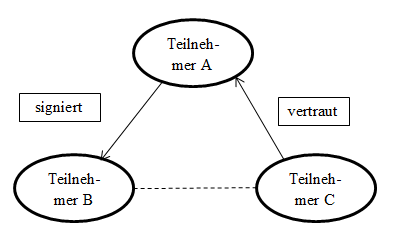
\includegraphics[width=0.4\textwidth]{images/WOT.png}
			\caption[Web of Trust Vertrauensmodell]{Web of Trust Vertrauensmodell\footnotemark}
			\end{wrapfigure}
			\footnotetext{\cite[In Anlehnung an:][S. 121]{Ertel2012}}
			Teilnehmer C möchte Teilnehmer B eine verschlüsselte Nachricht schicken. Dazu besorgt er sich zunächst das Zertifikat von Teilnehmer B. Dieser wurde zuvor von Teilnehmer A signiert. Da Teilnehmer C Teilnehmer A vertraut, beschafft sich Teilnehmer C den öffentlichen Schlüssel von Teilnehmer A und verifiziert mit diesem das Zertifikat von Teilnehmer B. Ist die Verifizierung erfolgreich, so kann Teilnehmer C den öffentlichen Schlüssel von Teilnehmer B vertrauen.
			
			Bei diesem Modell wird zwischen zwei Arten des Vertrauens unterschieden. Einerseits existiert das Vertrauen in eine Person bzw. dessen Signatur. Andererseits besteht ein Vertrauen in einen signierten Schlüssel eines Dritten, der von einer vertrauensvollen Person signiert wurde. Beide Arten des Vertrauens können unabhängig voneinander existieren.

		\section{Schlüsselaustausch}
			Für die sichere Kommunikation ist ein sicherer Schlüsselaustausch die Ausgangsbasis um Angriffe zu verhindern. \glqq erbei ist der geschützte Austausch geheimer Schlüssel symmetrischer Kryptosysteme von Interesse.\grqq\footcite[Vgl.][S. 437]{Eckert2013}
			\subsection{RSA - Rivest, Shamir und Adleman-Kryptosystem} 
				%Problem
				Beim klassischen Schlüsselaustausch werden die Sitzungsschlüssel durch den Public-Key innerhalb des Server-Zertifikat übertragen.\footcite[Vgl.][]{Boeck2013} Dies geschieht mittels \ac{RSA}-Verfahren. Verschlüsselte Kommunikation ist jedoch nur sicher, solange die Schlüssel geheim bleiben. Die Gefahr beim klassischen \ac{RSA}-\ac{PKI}-Verfahren ist, dass vergangene Kommunikation nachträglich zu jedem Zeitpunkt entschlüsselt werden kann, sobald Angreifer in Besitz des Private-Key sind.\medskip\\
				%Idee
			\subsection{PFS - Perfect Forward Secrecy}
				Im Gegensatz zum klassischen RSA-Schlüsselaustausch ist es sinnvoller, die Sitzungsschlüssel
				zum Einen nicht mehr zu übertragen und zum Anderen unabhängig voneinander ständig neu zu generieren und bei Terminierung zu löschen. Realisiert wird dies durch die Protokoll-Eigenschaft Forward Secrecy, die im Kryptographischen Fachjargon auch \ac{PFS}\footcite[Vgl.][]{Boeck2013} genannt wird. Die \glqq Forderung an die Verfahren und Protokolle zur Schlüsselerneuerung besteht darin dafür zu sorgen, dass die Kenntnis eines Schlüssels, also dessen Aufdeckung, nicht dazu führt, dass damit auch vorherige und nachfolgende Schlüssel direkt aufdeckbar sind.\grqq\footcite[Vgl.][S. 439]{Eckert2013} Wie notwendig \ac{PFS} geworden ist zeigen die jüngsten Ereignisse im Zusammenhang mit dem OpenSSL-Bug "Heartbleed", mit dem es sehr einfach war private Schlüssel von Servern auszulesen.\footcite[Vgl.][]{Zhu2014} \medskip\\
				%Umsetzung
				Das \ac{DHE} Verfahren ermöglicht dabei als Basis die Aushandlung eines Sitzungsschlüssels bei dem die Kommunikationspartner verschiedene Nachrichten senden und sich auf einen Sitzungsschlüssel einigen können, ohne diesen je übertragen zu haben. Dieser Schlüssel ist auch nur für die aktuelle Verbindung gültig und wird anschließend gelöscht. Der Public-Key des Servers wird weiterhin übertragen, jedoch nur um den Schlüsselaustausch zu signieren. \glqq geschlossene Sitzungen können somit im Nachhinein nicht mehr entschlüsselt werden.\grqq \footcite[Vgl.][]{Schulz2014} Die Verschlüsselungsverfahren \ac{TLS/SSL} und \ac{IPsec} beherrschen bereits \ac{PFS}.\medskip\\
				%Vorteile
				Aufgezeichnete verschlüsselte Daten können somit bei Besitz des privaten Schlüssels nicht entschlüsselt werden. Zudem wird einfaches Belauschen einer aktiven Verbindung deutlich erschwert, denn es müsste die gesamte Kommunikation mit einem gezieltem \ac{MITM}-Angriff manipuliert werden. Für diese Problematik gibt es wiederum moderne Ansätze wie \ac{DANE} (Vgl. Kapitel \ref{subsec:dane}), die in Kombination mit \ac{PFS} aktuell bei der Verschlüsselung von Verbindungen höchsten Sicherheitsansprüchen entsprechen, indem zusätzlich die Authentizität der Kommunikation gewährleistet wird.\medskip\\
				%Nachteile
				Nachteile gibt es lediglich bei der Verwendung des bereits überholten, und seit Jahren als geknackt bekannte \ac{DHE}-Verfahren, denn dabei verzögert sich zusätzlich der Verbindungsaufbau. Die Schlüssellänge ist Minimum 1024 Bit, und längere Schlüssel mit 2048 oder 4096 Bit sind dabei nicht sicherer.\footcite[Vgl.][]{Boeck2013} Der moderne Nachfolger mit elliptischen Kurven \ac{ECDH} gilt aktuell als sicher und benötigt dabei weniger als 1024 Bit und verzögert den Verbindungsaufbau nur unweigerlich.\medskip\\
				%Grenzen
				Obwohl es Forward Secrecy bereits seit 1999 im \ac{TLS} Standard 1.0\footcite[Vgl.][]{Boeck2013} vorgesehen ist, und somit essentieller Bestandteil von Verschlüsselung ist, hat sich \ac{PFS} noch nicht als Standard durchgesetzt.\footcite[Vgl.][]{SSLLabs} Dies liegt zum einen an den Webservern. Mit einem Apache Webserver ist nur eine Länge des Modulo (Modulus) von 1024 Bit vorgesehen. Beim Einsatz von \ac{DHE} würden Provider damit ihre Server daher unsicher betreiben. Zum Anderen sind es auf Client-Seite die Browser die \ac{DHE} bzw. \ac{ECDH} lange Zeit ignoriert haben. Der Internet Explorer verschlüsselte nur nach DSS, wobei der de-facto Standard für Verschlüsselung bereits \ac{RSA} war. Opera unterstützte lediglich das überholte \ac{DHE}-Verfahren und Safari priorisiert Forward Secrecy niedrig und bevorzugt bei gegebener Option sogar die unverschlüsselte Kommunikation. Lediglich Firefox und Chrome unterstützen \ac{PFS} in vollem Umfang.\medskip\\
				%Browser prüfen und mit eigenen Quellen versehen
				Für die E-Mail Kommunikation ist \ac{PFS} essenziell für die Befriedigung hoher Sicherheitsbedürfnisse. Um die dazugehörigen Sicherheitsniveaus abzudecken müssen E-Mail-Server Forward Secrecy unterstützen. Im August 2013 war \ac{PFS} nur sporadisch verbreitet in der E-Mail-Kommunikationslandschaft.\footcite[Vgl.][]{Schulz2014} Mittlerweile wird von vielen E-Mail-Providern auch \ac{PFS} angewandt. Die Umsetzung erfolgt jedoch noch zu zögerlich, wenn man die Tatsache betrachtet, dass \ac{PFS} im Zusammenhang mit Heartbleed der letzte Funken Hoffnung für betroffene Nutzer war, das zumindest vergangene Kommunikation nicht entschlüsselt werden kann.\footcite[Vgl.][]{Zhu2014}
		
		\section{Informationsverschlüsselung}
			Für hohe Sicherheitsanforderungen entscheidend ist die Vertraulichkeit und Integrität der Datenkommunikation zwischen zwei Endpunkten. In der E-Mail-Kommunikation wird dies mit sog. Ende-zu-Ende-Verschlüsselung (englisch \ac{E2EE}) und den Diensten \ac{S/MIME} und \ac{PGP} realisiert, die im Nachgang beleuchtet werden.
			Es gibt mittlerweile verschiedene Möglichkeiten \ac{E2EE} umzusetzen. Im Grunde müssen durch die Nutzer jedoch Einstellungen in den E-Mailprogrammen wie Thunderbird, Outlook oder Mail.app vorgenommen werden oder zusätzliche Software installiert werden. Demzufolge besteht ein erhöhter Einrichtungsaufwand für die Endnutzer zur Sicherstellung der Vertraulichkeit und um in Sicherheitsniveaus der Stufe 3 oder 4 (Vgl. \prettyref{tab:sicherheitsniveaus}) zu kommunizieren. Allerdings ist \ac{E2EE} \textit{essenziell} zur Erreichung dieser Stufen\medskip
			Erste E-Mail-Provider gehen zum Teil eigene Wege wenn es um die Gestaltung von benutzerfreundlicher \ac{E2EE} geht. Google bspw. arbeitet an einer Erweiterung im eigenen Chrome Browser um mittels OpenPGP zu verschlüsseln.\footcite[Vgl.][]{Somogyi2013}. Aber auch kleinere Anbieter sind an der Umsetzung für ihre Webmailer\footcite[Vgl.][]{Posteo2013} und somit \ac{E2EE} deutlich benutzerfreundlicher zu machen. 
			
			\subsection{PGP - Pretty Good Privacy}
			\label{subsec:pgp}
				%Problem + Idee
				Im Jahre 1991 wurde dem US Senat ein Gesetz vorgelegt, welches vorsieht, dass jede Verschlüsselungssoftware staatliche Zugriffe ermöglichen müsse. Daraufhin entwickelte Phil Zimmermann noch im selben Jahr die erste Version von \ac{PGP}, die diese Hintertür nicht bot.\footcite[vgl.][S. 29]{Schwenk}
			
				Die Softwarefamilie \acl{PGP} stellt ``...Dienste zur digitalen Signatur und zur Verschlüsselung von Nachrichten...''\footcite{Mueller2011} zur Verfügung und ist damit für die Vertraulichkeit der Informationen verantwortlich.
				
				Allerdings wurden diese Bemühungen erst nach sieben Jahren Entwicklung, diversen Anklagen gegen Zimmermann und die anderen Beteiligten sowie das Herausbringen zahlreicher nationaler (US-Amerikanischer) und internationaler Versionen als internationaler Standard \textit{OpenPGP} angesehen.\footcite[][S. 29-35]{Schwenk}
				\medskip
				
%				Mit PGP werden kryptographische Dienste bereitgestellt die unter anderem Dateiverschlüsselung, Schlüssel-Recovery und das Signieren von Dokumenten umfassen.
				
				%Umsetzung
				Um die Integrität einer E-Mail zu gewährleisten, wird zuerst ein zufälliger Schlüssel (Shared Secret) erzeugt. Anschließend wird die E-Mail Nachricht mit diesem symmetrisch verschlüsselt. Danach wird das Shared Secret selbst mit dem öffentlichen Schlüssel des Empfängers asymmetrisch verschlüsselt und der verschlüsselten E-Mail voran gehangen. Soll die E-Mail mehrere Empfänger erreichen, so wird der letzte Schritt wiederholt.\footcite[vgl.][S. 43]{Schwenk}
				\medskip
				
				
				Ein entsprechendes Programm zur Implementierung des OpenPGP Standards ist \ac{GPG}. Dieses Tool ist für gängige E-Mail-Clients verfügbar und ermöglicht die Verschlüsselung und den Schlüsselaustausch so benutzerfreundlich wie möglich zu gestalten. Denn der Austausch der öffentlichen Schlüssel muss noch manuell erfolgen.
				\medskip
				%Zu Berücksichtigen ist hierbei der Faktor, dass Private Keys nur lokal gespeichert und durch sichere Passphrasen geschützt sind.
				
							
%				- dabei handelt es sich um RFC 2440, welcher "die Struktur aller PGP-Nachrichten und auch die Prozeduren zu ihrer Generierung" beschreibt
%				- Basis ist Version 5.0 von PGP
%				\footcite[][S. 42]{Schwenk}
%				\medskip\\

%				Für das Format zur Verschlüsselung und Signierung von Daten nach \ac{PGP} 5 bietet OpenPGP einen Standard nach \acs{RFC} 4880.

				
%				Ab Version 5.0 wird in PGP neben \ac{RSA} auch \ac{DHE} zum Austausch symmetrischer Schlüssel und eine symmetrische Blockchiffre für die Mailverschlüsselung verwendet. Die Integrität \glqq Authentizität [der Daten] wird durch die Verwendung von \ac{SHA}-1 und \ac{MD5} als Hashfunktionen bzw. als \ac{MAC}s sichergestellt.\grqq\footcite[S.823]{Eckert2013}\medskip				
				
				
				%Vorteile
				Ein Vorteil von \ac{PGP} liegt darin, dass es sowohl auf dem dezentralen Vertrauensmodell Web of Trust als auch auf dem hierarchischen Vertrauensmodell der \ac{PKI} basiert.\footcite[vgl][S. 38f.]{Schwenk}
				Außerdem werden die verschlüsselten Nachrichten vor dem Versenden komprimiert und verringern dadurch nicht nur Traffic, sondern verbessern somit auch den Schutz vor Angreifern.\footcite[][S. 45]{Schwenk}	
				Des Weiteren steht der Sourcecode von \ac{PGP} öffentlich zur Verfügung und kann beliebig auf Richtigkeit überprüft werden.\footcite[][S. 47]{Schwenk}
				\medskip
									
				
				%- ADK hinzufügen --> bezieht sich auf Unternehmen, daher nicht mit eingefügt
				%\footcite[][S. 32]{Schwenk}
				%\medskip				
			
			
				%Nachteil
				Der öffentliche Sourcecode stellt jedoch gleichzeitig auch einen Schwachpunkt dar, da es somit Angreifern ermöglicht wird, potenzielle Schwachstellen und Sicherheitslücken in der Implementierung aufzufinden. Vor allem mit der Zunahme neuer Features wird dieser Nachteil erheblicher, was durch Angriffe von Senderek, Klíma und Rosza bewiesen wurde.\footcite[vgl.][S. 47-55]{Schwenk}
				
				Ein weiterer Nachteil liegt in der Schwierigkeit beim Austausch von Schlüsselinformationen für \ac{E2EE}. Dies muss noch manuell mit Hilfe von Software erfolgen und ist daher noch nicht Standard heutiger E-Mail-Kommunikation. 
				Es gibt zwar die Möglichkeit private Schlüssel durch Dienste\footnote{Bspw. iMessage von Apple für Instant Messaging} zu verteilen, jedoch ist diese Methode umstritten. Sie bietet zwar Ende-zu-Ende Verschlüsselung, allerdings ist der eigentliche Sinn des privaten Schlüssels verfehlt, wenn der Dienst bzw. Provider diesen für den Nutzer bestimmt und auf dem eigenen Server zwischenspeichert. Der Anwender hat keinen Einfluss auf den privaten Schlüssel und ist damit nicht Eigentümer dieses Schlüssels, der in Folge dessen kein Private Key ist.\\
				Selbst vereinzelte \ac{CA}s gehen mit solcher Methodik vor\footcite{Kaps2014}, und untergraben damit die Sicherheit des ganzen \ac{CA}-Modell. \medskip\\
				
				%Bezug zu Sicherheitsniveaus
				Nichtsdestotrotz ermöglicht \ac{PGP} durch die  Ende-zu-Ende-Verschlüsselung, dass die Inhalte der E-Mail nur für den Sender und den rechtmäßigen Empfänger einsehbar sind. Daher ist es geeignet streng vertrauliche Informationen zu versenden.
				\medskip

				%Mail Bezug	
%				- Mail Plugin sucht in einer pubring.pkr Datei über die Mail Adresse des Empfängers nach dessen öffentlichen Schlüssel
%				- Vorteil hierbei ggü. S/MIME ist dass einem Öffentlichen Schlüssel mehrere Mail Adressen zugeordnet werden können
%				\footcite[][S. 40]{Schwenk}
%				
%				- PGP als Produkt liefert ein E-Mail Plugin mit für Outlook, Outlook Express und Eudora
%				%hier gibt es bestimmt mittlerweile noch weitere 	
%				- Buttons für 1 Klick Verschlüsselung/Entschlüsselung
%				- PGP Menü für spezifischere Einstellungen
%				\footcite[][S. 38]{Schwenk}
%				
%				
%				- eigenen öffentlichen Schlüssel versenden?
%				\footcite[][S. 40]{Schwenk}
%				
%				- Ende zu Ende Verschlüsselung und daher geeignet für Stufe 4
				
	
			\subsection{S/MIME - Secure / Multipurpose Internet Mail Extensions}
			
				%Problem
				Die bislang betrachteten Verfahren bieten keine Möglichkeit einer \ac{E2EE}. \ac{PGP} hat als erstes Protokoll diese Lücke gefüllt. Mit \ac{S/MIME} kam 4 Jahre später ein zweiter Standard hinzu.\footcite[Vgl.][]{Duevel}
				\medskip\\
							
				%Idee
				\ac{S/MIME} ist eine Erweiterung des MIME Datentyps, der für die Signierung und/oder Verschlüsselung von Nachrichten entwickelt worden ist.
				Bislang konnten E-Mails nur im ASCII-Zeichensatz versendet werden. Mit dem Anbruch des digitalen Zeitaltern stieg jedoch die Forderung auch andere Datentypen austauschen zu können. \ac{S/MIME} setzt dieses Bedürfnis um.\footcite[Vgl.][S. 57-60]{Schwenk}
				\medskip
				
				%Voraussetzung
				Damit ein Nutzer \ac{S/MIME} verwenden kann, benötigt er ein X.509 Zertifikat. Dieses wird in seiner einfachsten Form kostenlos von einer \ac{CA} ausgestellt.\footcite[Vgl.][]{Duevel}
				
				Das eigene Zertifikat kann ein Nutzer mit anderen austauschen, indem er es einer signierten E-Mail anfügt. Ein E-Mail Client kann dieses automatisch in seine Zertifikatsdatenbank ablegen. Der genaue Prozess hierfür ist im Schwenk\footcite[][S. 65 ff.]{Schwenk} beschrieben.
				\medskip
														
				%Umsetzung
				Hat sich der Absender für die Verschlüsselung via \ac{S/MIME} entschieden, sucht der Mail Client automatisch in der Zertifikatsdatenbank nach einem Zertifikat, welches die E-Mail Adresse des Empfängers enthält. Sollte ein solches Zertifikat nicht gefunden werden, wird der Nutzer darüber informiert, dass eine \ac{S/MIME} Verschlüsselung nicht möglich sei. Ist ein entsprechendes Zertifikat vorhanden, wird die E-Mail hybrid verschlüsselt.\footcite[][S. 65]{Schwenk}
				
%				- Bedeutet, dass Nachricht symmetrisch verschlüsselt wird und das Shared Secret mit dem im Empfänger-Zertifikat angegebenen öffentlichen Schlüssel verschlüsselt wird
%				- Anschließend base64 codiert, damit Mailserver den Inhalt nicht unbeabsichtigt ändern kann
				
				Um die Lesbarkeit von \ac{S/MIME} signierten E-Mails auch für Nutzer zu gewährleisten, die dieses Verfahren nicht verwenden, stehen zwei verschiedene Datentypen zur Verfügung. Auf eine genauere Beschreibung soll an dieser Stelle verzichtet und stattdessen auf den Schwenk\footcite[Vgl.][S. 65]{Schwenk} verwiesen werden.
				\medskip
				
%Zwei verschiedene Datentypen für Signatur beschreiben?

%				- es stehen zwei Datentypen zur Verfügung: application/pkcs-mime signedData und multipart/signed
%				- application/pkcs-mime besteht aus einem einzigen Element, welches die verschlüsselten Daten, die Signatur + weitere Zusatzinformationen enthält
%				- liegt im PKCS\#7 Format vor und kann daher nur von Clients interpretiert werden, die dieses Format unterstützen
%				- Bietet dafür ein höheres Maß an Integrität und Authentizität, der Inhalt kann nicht versehentlich durch Mailserver verändert werden
%				- multipart/signed besteht aus zwei Elementen
%				- erster Teil sind signierte Daten in Form eines MIME-Objektes und daher von jedem Client interpretierbar
%				- zweiter Teil enthält die eigentliche Signatur in PKCS\#7 Format
%				- Dadurch ist die Nachricht für alle Clients interpretierbar, allerdings kann der erste Teil durch Mailserver versehentlich geändert werden
%				\footcite[][S. 65]{Schwenk}

				
										
				%Vorteile
				Der Vorteil von \ac{S/MIME} liegt darin, "dass Verschlüsselung und Signatur genauso einfach zu bedienen sind, wie z.B. [..] das Anfügen eines Attachments"\footcite[Vgl.][S. 61]{Schwenk}. Außerdem wird \ac{S/MIME} durch viele Browser by Default unterstützt.\footcite[Vgl.][]{Duevel}
				Durch die zwei verschiedenen Datentypen, können \ac{S/MIME} signierte Nachrichten auch von E-Mail Clients interpretiert werden, die dieses Verfahren nicht verwenden. 
				\medskip
				
				Da \ac{S/MIME} genau wie \ac{PGP} eine \ac{E2EE} ermöglicht, ist auch dieses Verschlüsselungsverfahren für das Versenden von streng vertraulichen Informationen geeignet.
				\newpage
				
				
		\section{Transportwegverschlüsselung}
			Das \ac{SSL}-Protokoll wurde zunächst durch die Firma Netscape entwickelt, um die Kommunikation über \ac{HTTP}-Verbindungen abzusichern.\footcite[Vgl.][S. 796]{Eckert2013} \ac{SSL} kann auf der Sitzungs- und Präsentationsschicht des \ac{OSI}-Referenzmodells angesiedelt werden und setzt meist auf dem \ac{TCP} auf. Es hat die Aufgabe den darüber liegenden Schichten die Möglichkeit für eine authentifizierte, integritätsgeschützte und verschlüsselte Kommunikation zu geben.\footcite[Vgl.][S. 799 ff.]{Eckert2013}
			Die Version \ac{SSL} 3.0 hat sich mittlerweile als de facto Standard im Internet durchgesetzt und wird von allen gängigen Browsern unterstützt.\\
		
			\begin{wrapfigure}{r}{0.4\textwidth} %wrapfigure ist eine Umgebung, in dem eine Abbildung von TExt umgeben werden kann; {r} steht für rechts, {l} geht auch; zweites Argument ist die Breite des "Einfügekastens"
				\centering
				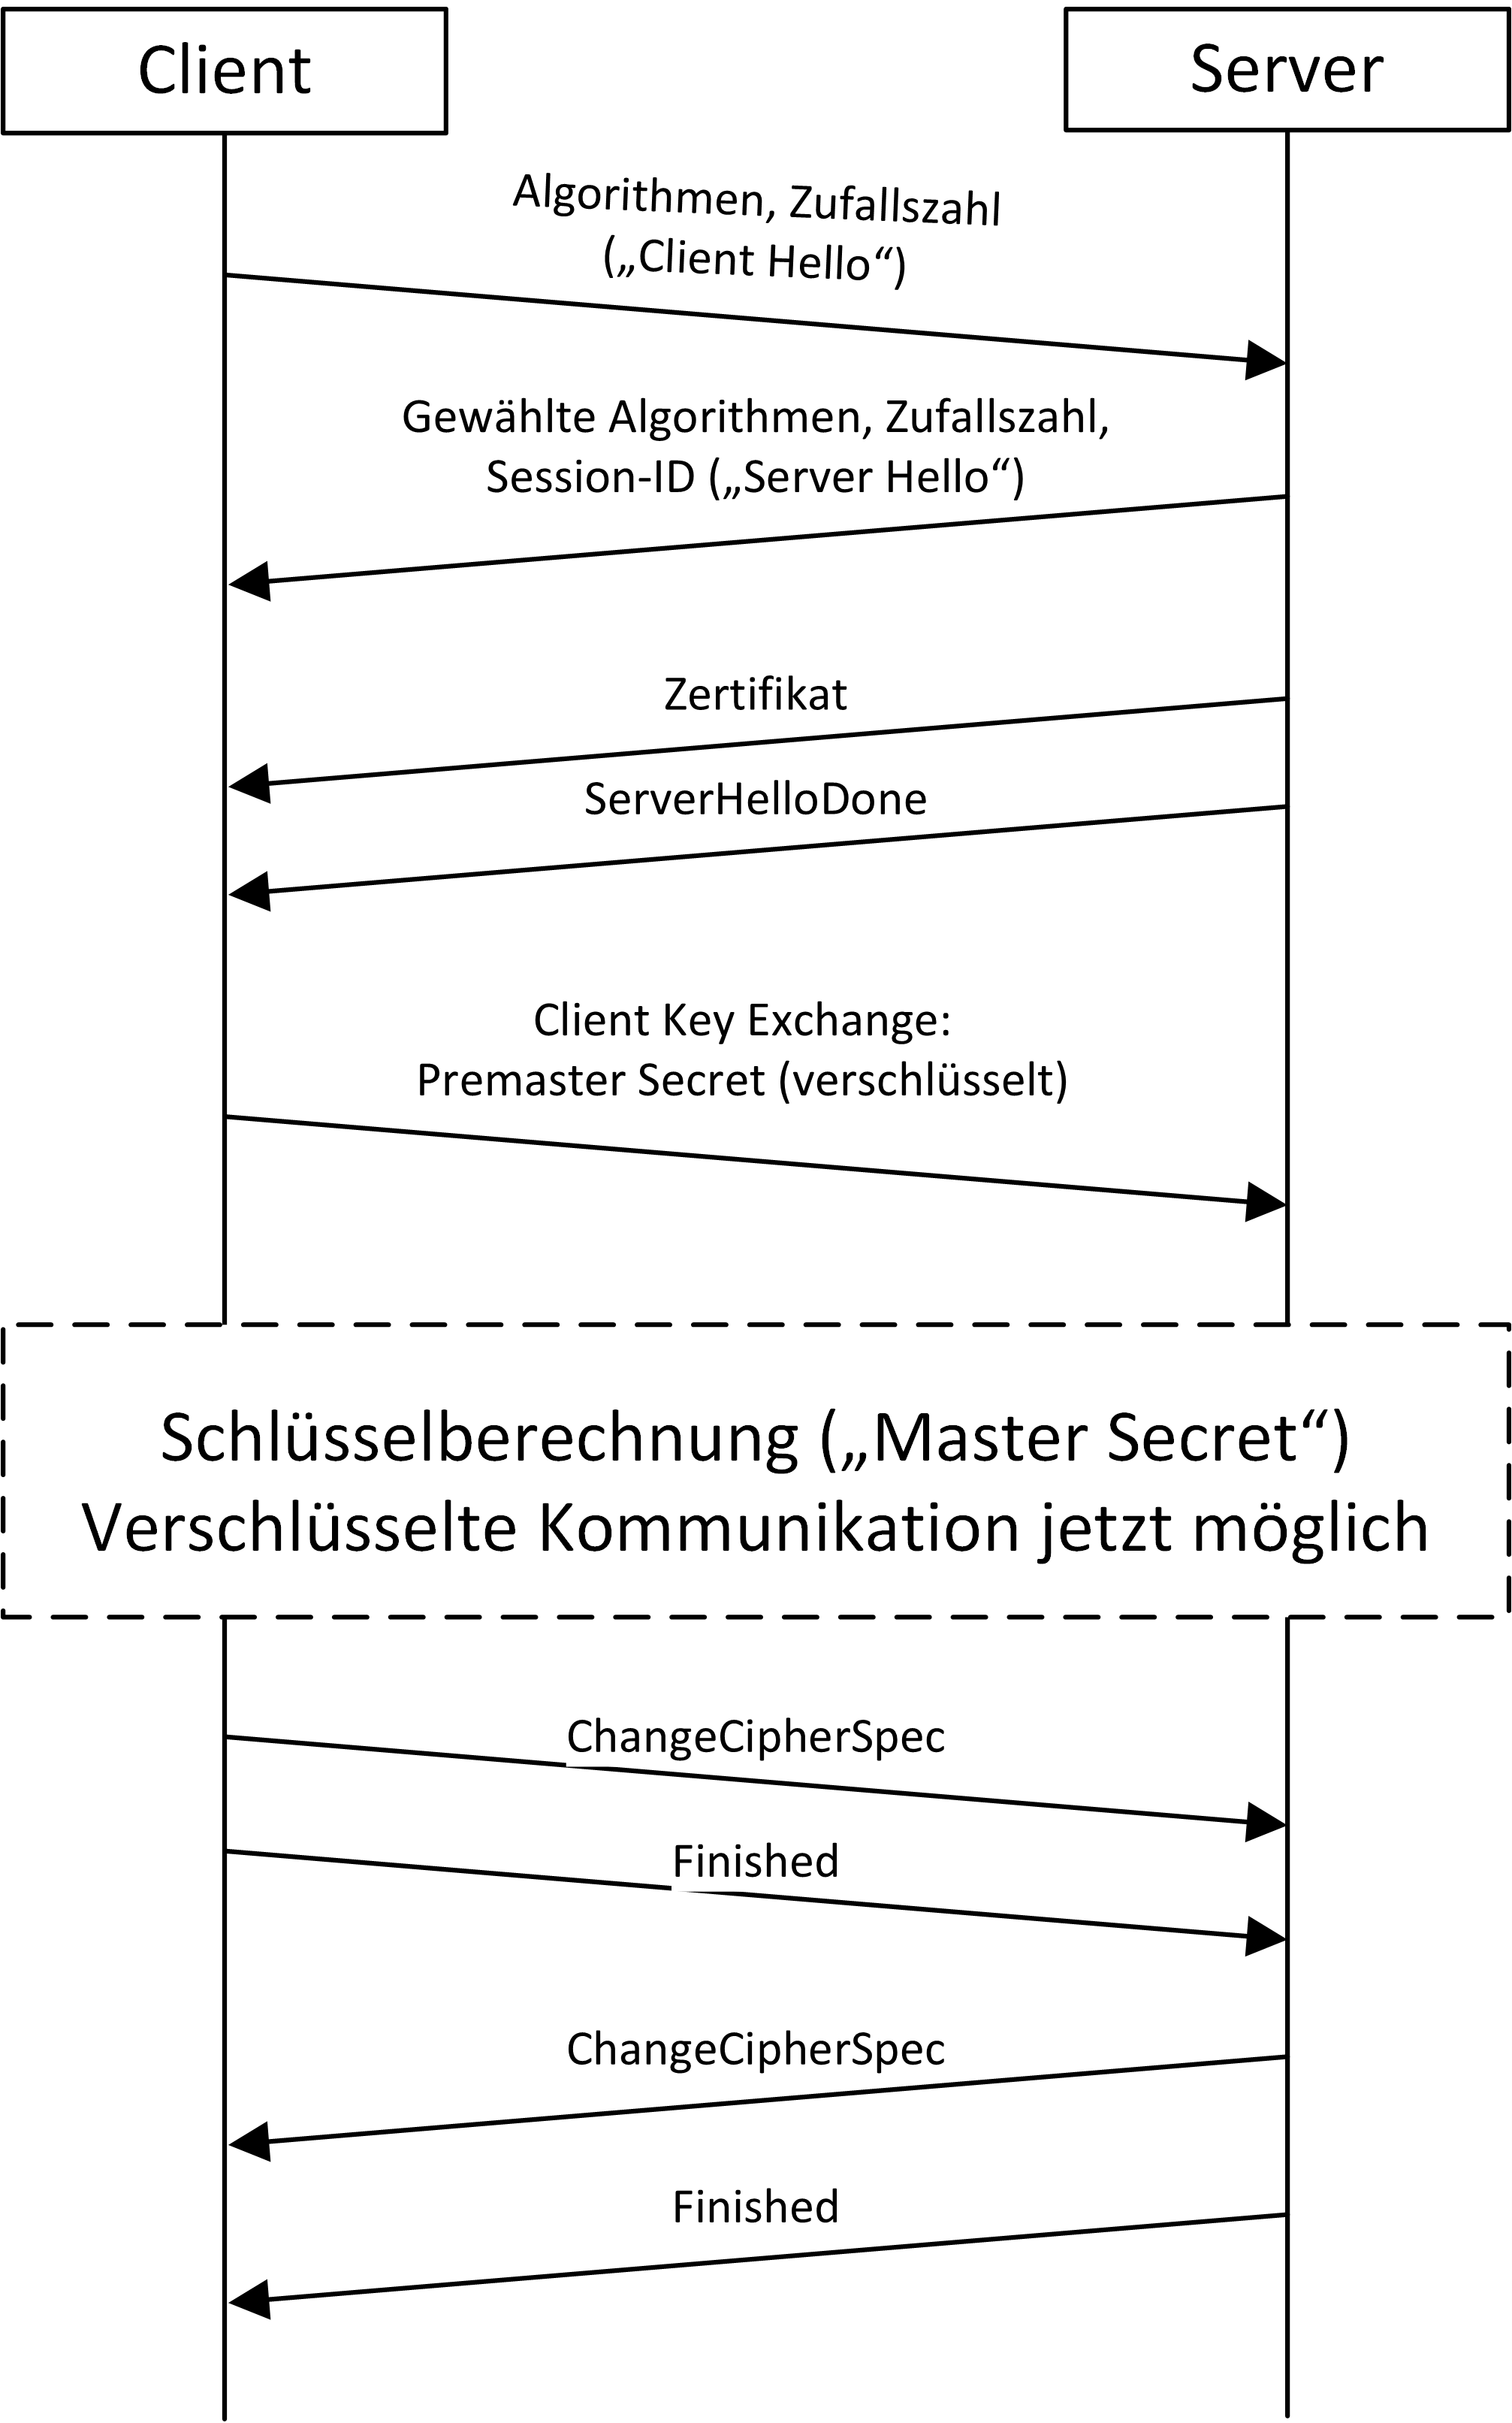
\includegraphics[width=0.4\textwidth]{images/MSC_Transport.png}
				\caption[Handshake-Protokoll mit RSA]{Handshake-Protokoll mit RSA\footnotemark} %Bildunterschrift, erstes Argument ist für Abbildungsverzeichnis ohne Fußnote; \footnotemark ist ein Platzhalter für die Fußnote
				\label{img:MSC_Transport} %für Bezüge auf diese Abbildung
			\end{wrapfigure}\footnotetext{\cite[In Anlehnung an][S. 170]{Sorge2013}} 
			Das \ac{TLS}-Protokoll kann als Weiterentwicklung von \ac{SSL} 3.0 angesehen werden und liegt aktuell in der Version 1.2 vor.
			Da beide Protokolle in ihren Kernkonzepten übereinstimmen werden sie häufig synonym verwandt. Da \ac{TLS} jedoch eine Weiterentwicklung von \ac{SSL} ist, werden dort einige Erweiterungen eingeführt sowie unsichere Verfahren zur Berechnung von \ac{MAC}-Werten durch neuere Varianten ersetzt.\\
		
			%\begin{figure}
			%	\begin{minipage}{0.5\textwidth}
			%		\centering
			%		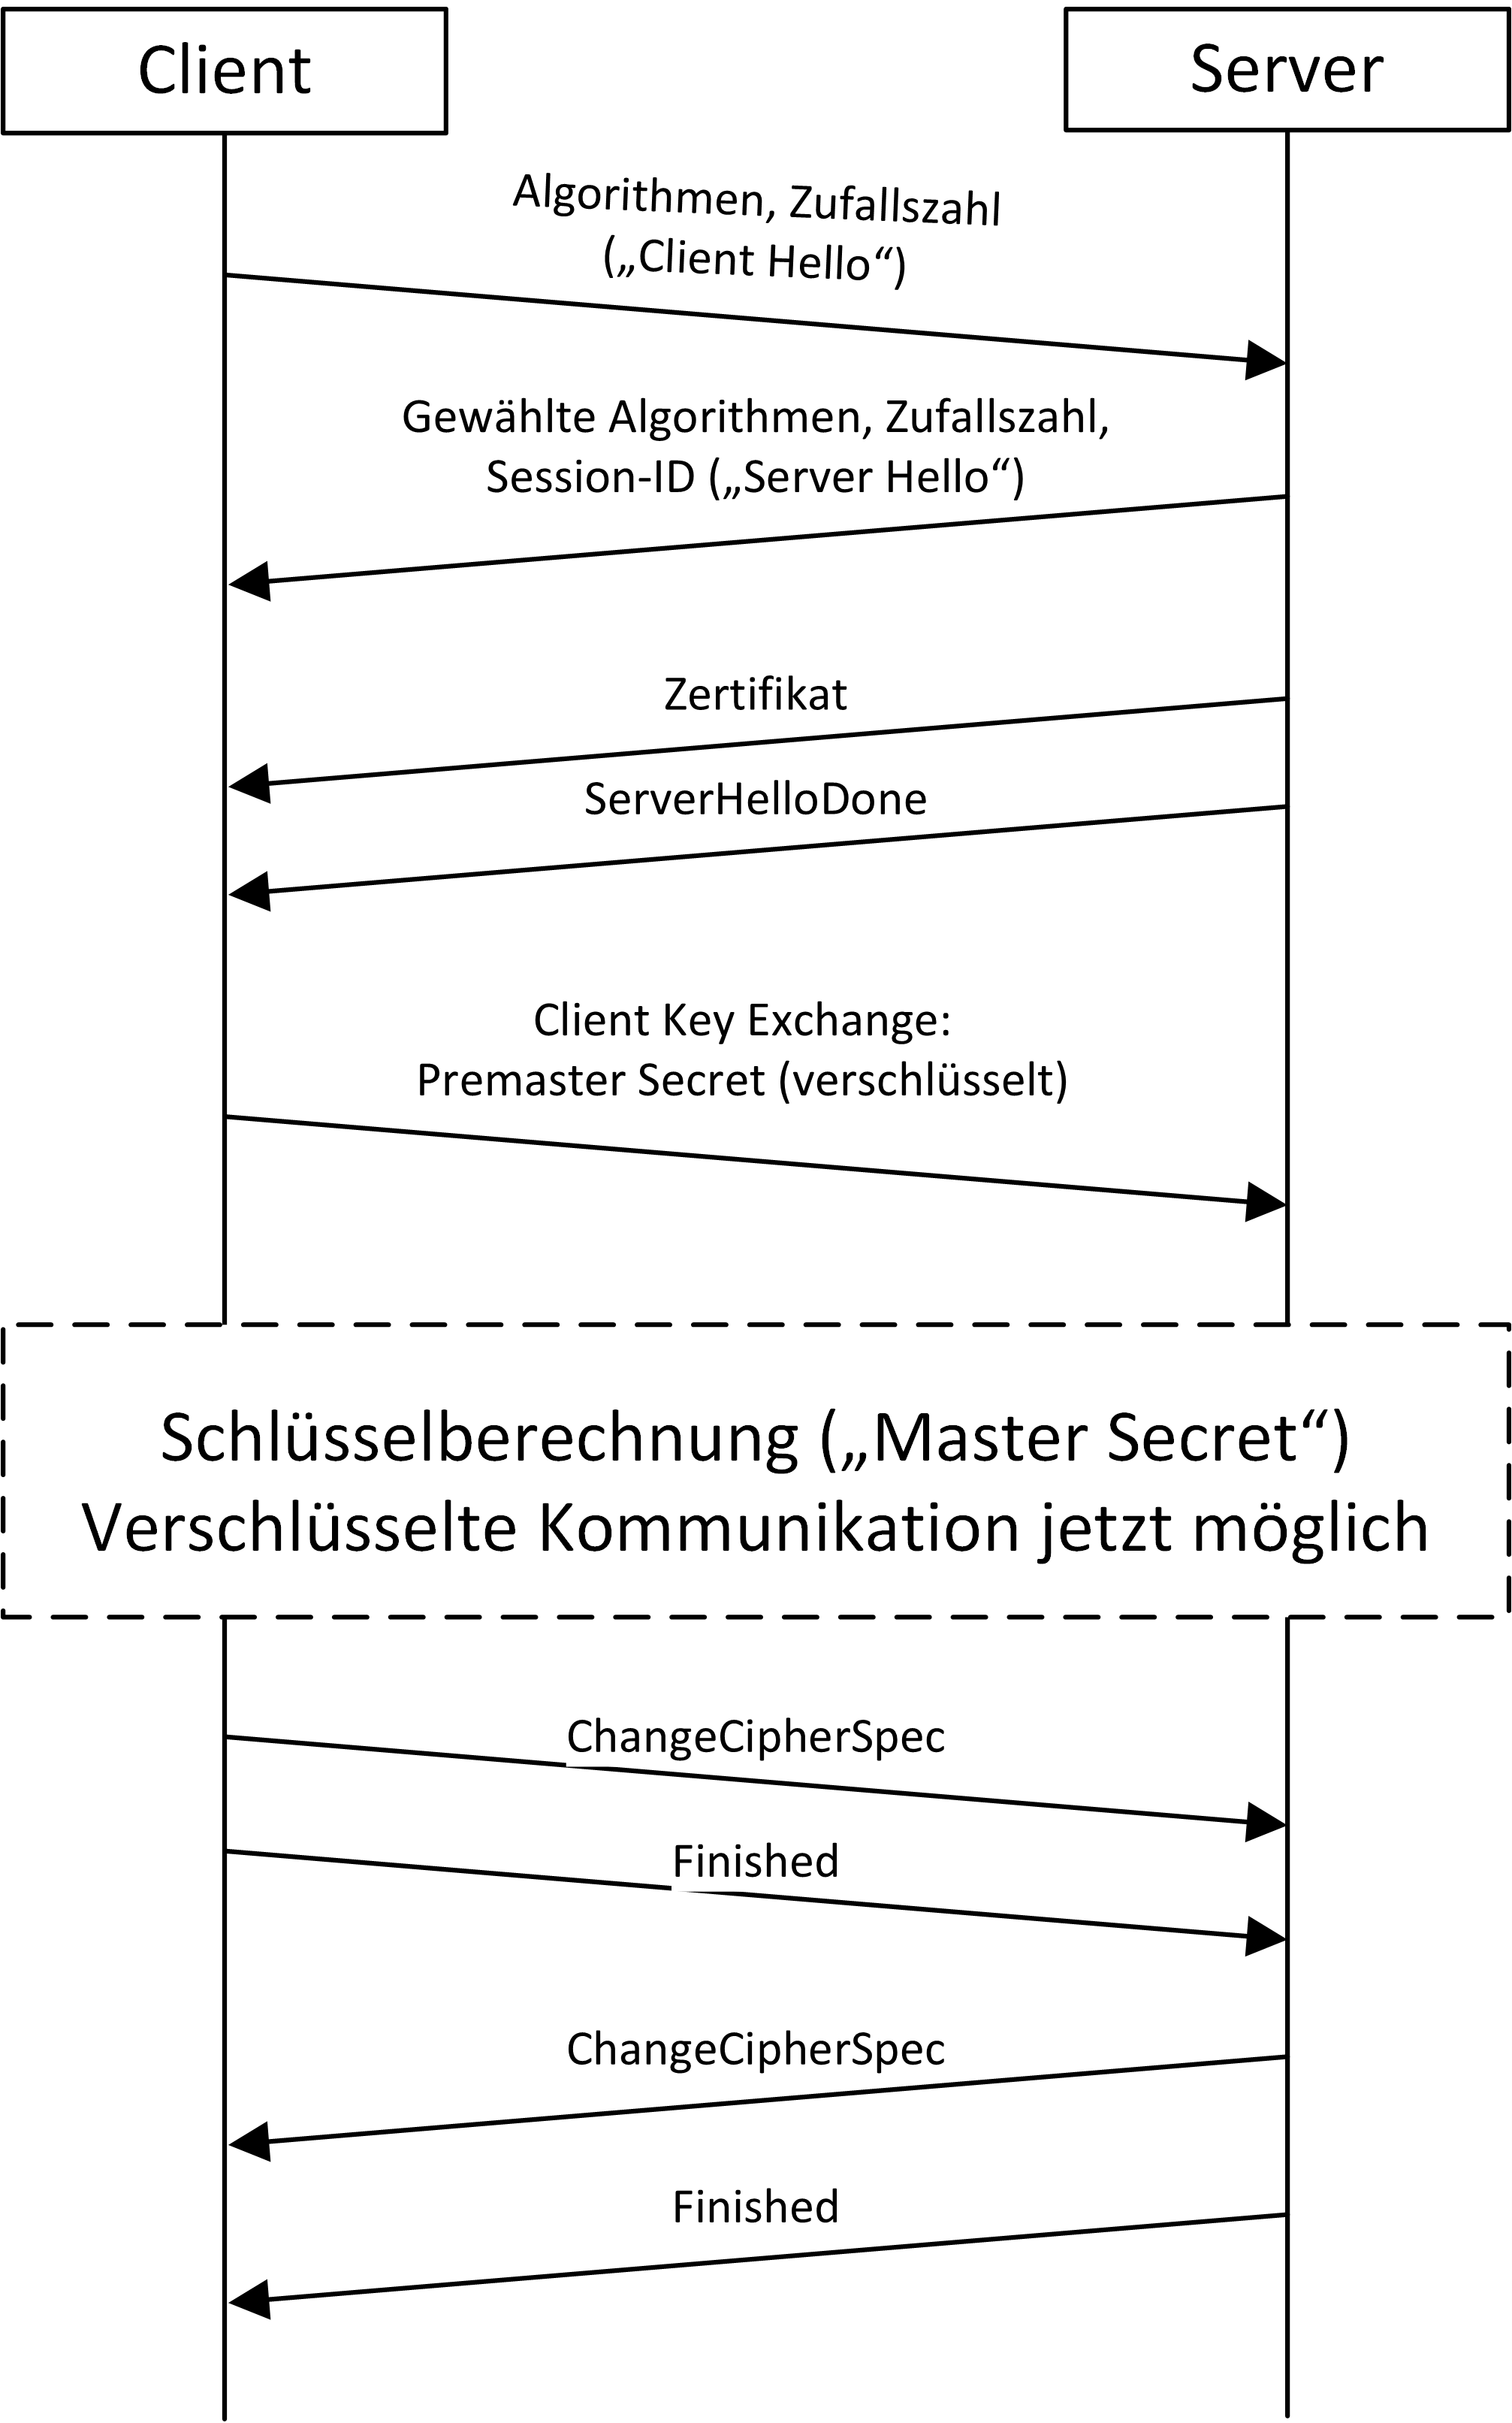
\includegraphics[width=0.45\textwidth]{images/MSC_Transport.png}
			%		\caption[Handshake-Protokoll mit RSA]{Handshake-Protokoll mit \ac{RSA}\footcite[In Anlehnung an:][S. 170]{Sorge2013}}
			%	\end{minipage}
			%\end{figure}
			
			Beide Protokolle bestehen aus mehreren Schichten bzw. Unterprotokollen wobei das Record- und das Handshakeprotokoll von besonderer Bedeutung sind. 
			Das Record-Protokoll ist für die Fragmentierung, Authentifizierung mittels \ac{MAC} und Verschlüsselung der zu übertragenden Daten zuständig. 
			Mittels des Handshakeprotokolls werden Sitzungen zwischen den Kommunikationspartnern hergestellt. 
			Dies bedeutet, dass die Kommunikationspartner durch den Austausch von Zertifikaten authentifiziert werden können und alle Informationen, die zur Berechnung des Shared Secret für die symmetrische Verschlüsselung der Daten benötigt werden, ausgetauscht werden. 
			Abbildung \ref{img:MSC_Transport} verdeutlicht den schematischen Ablauf eines solchen Sitzungsaufbaus unter Verwendung von \ac{RSA} für den Schlüsselaustausch.\\
			
			Durch die flexible Gestaltung des Handshake-Protokolls wird gleichzeitig auch die Komplexität von \ac{TLS/SSL} stark erhöht. 
			Dies hat zur Folge, dass durch die hohe Komplexität nicht mit Sicherheit alle Schwachstellen beim Design des Protokolls entfernt werden konnten. 
			Außerdem ist zu bedenken, dass \ac{TLS/SSL} aufgrund seiner weiten Verbreitung ein lohnendes Ziel für Angriffe ist. Die Sicherheit des Protokolls hängt dabei stark von den genutzten kryptologischen Methoden ab. 
			Außerdem ist zu beachten, dass es sich, aufgrund der Ansiedlung des Protokolls unterhalb der Anwendungsschicht, nur um eine Verschlüsselung der transportierten Nutzdaten auf dem Transportweg handelt. 
			Die Daten werden am Kommunikationsendpunkt entschlüsselt und anschließend an die entsprechende Anwendung weitergereicht.
			Dies bedeutet für die Anwendung im Bereich des E-Mailversands, dass die Nachrichten weiterhin im Klartext auf den Servern der Mailprovider vorliegen und von jedem, der berechtigten oder unberechtigten Zugang zu diesen erhält, ausgelesen werden können.
			Im Sinne der definierten Sicherheitsniveaus ist die \ac{SSL}-Verschlüsselung daher auf der zweitniedrigsten Stufe anzusiedeln, da das Mitlesen der versandten Mails zwar erschwert, aber nicht unmöglich gemacht wird.\\
			
			%\acp erzeugt den Plural des Akronyms bzw. hängt ein "s" an
			Auch die Authentifizierung der Kommunikationspartner mittels Zertifikaten weißt dieselben Schwachstellen durch die Vertrauensbeziehung zu bekannten \acp{CA}, die unzureichend gesichert sind, auf.  
			%Hier noch ein kurzer Abschnitt zu Metadaten mit Bezug auf die Schwachstellen (sec:metadaten)
	\section{DNS - Domain Name System}
	\label{sec:dns}
		Das \ac{DNS} ist ein wichtiger Dienst im Internet, da er dafür zuständig ist, gut merkbare Domainnamen in \ac{IP}-Adressen, und umgekehrt, aufzulösen.
		Um diese Auflösung bewerkstelligen zu können ist \ac{DNS} in einer Baumstruktur aufgebaut.
		
		\begin{wrapfigure}{l}{0.55\textwidth}
			\vspace{-12pt}
			\centering
			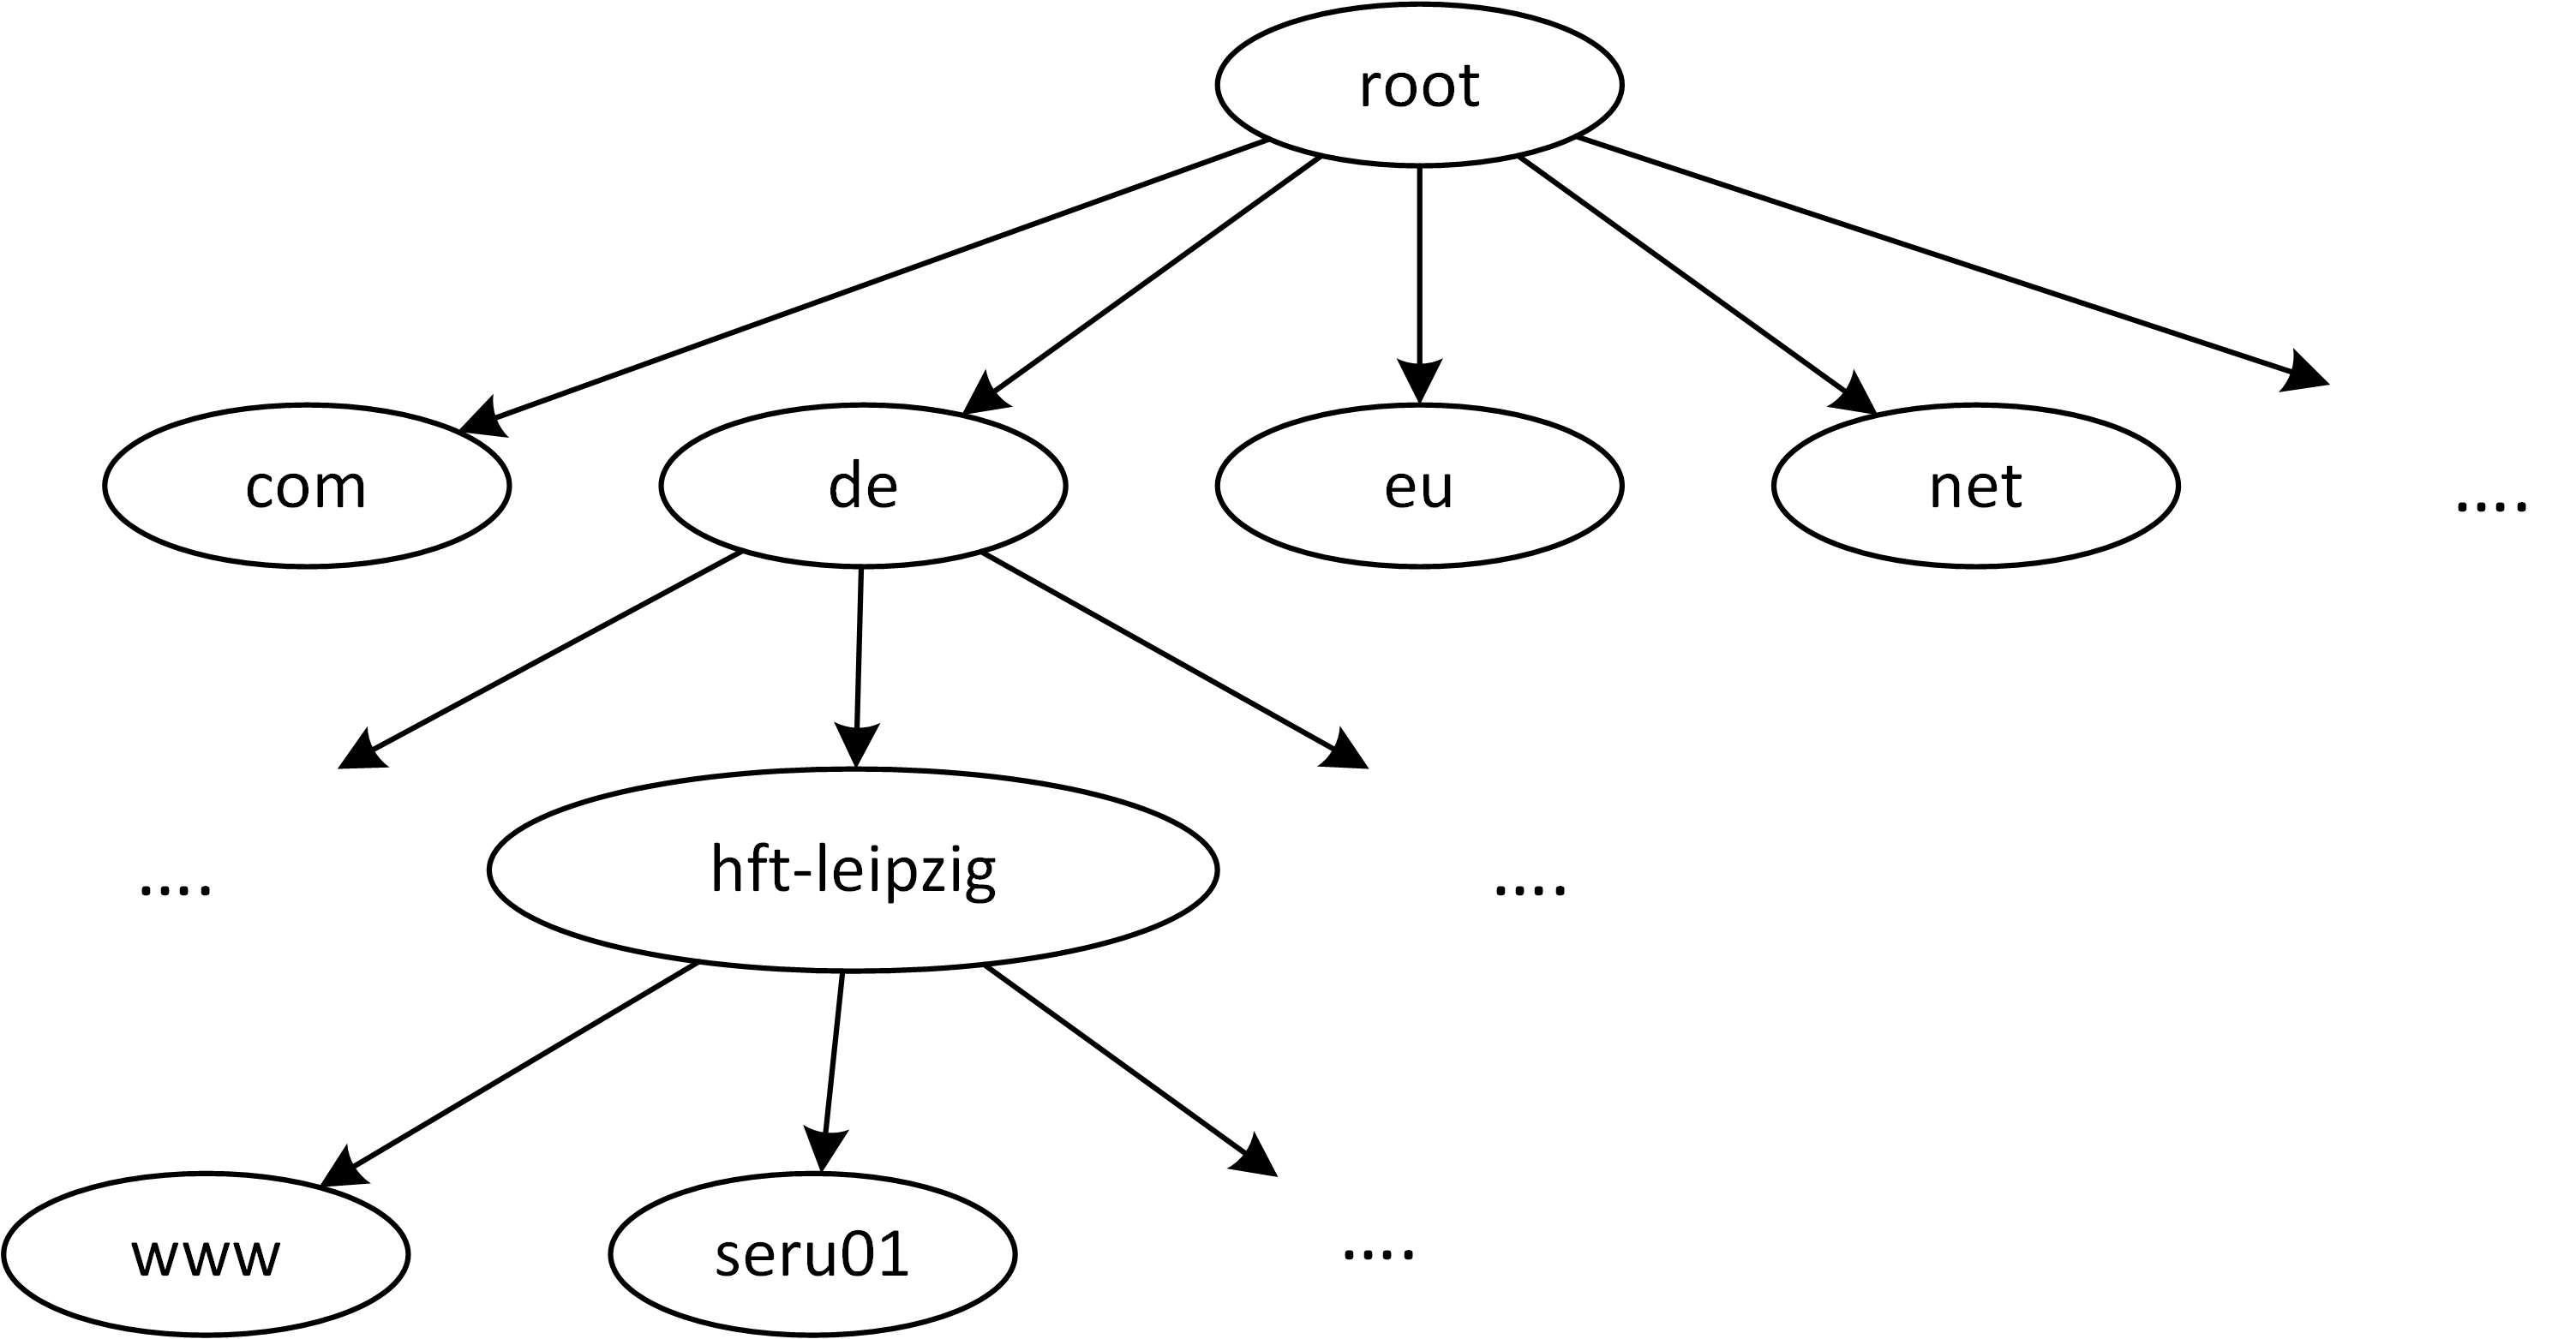
\includegraphics[width=0.55\textwidth]{images/Baumstruktur_DNS.png}
			\caption[Baumstruktur des DNS]{Beispielhafte Abbildung der Baumstruktur des \ac{DNS}\footnotemark}
			\label{img:baumstruktur_dns}
			\vspace{-12pt}
		\end{wrapfigure}\footnotetext{\cite[In Anlehnung an][S. 180]{Sorge2013}}
		
		Wie in Abbildung \ref{img:baumstruktur_dns} veranschaulicht, ist auf der obersten Ebene der Knoten \glqq root\grqq{} zu finden.
		Dies ist sozusagen die Wurzel des \ac{DNS} und hier finden sich auch die Root-Server des \ac{DNS}.
		Auf der nächsten Ebene kommen die \ac{TLD}, anschließend folgen die Second-Level-Domains und zum Aufbau einer gängigen \ac{URL} für \ac{HTTP} fehlt noch eine weitere Ebene, die den Hostnamen enthält.
		Soll ein Domainnamen aufgelöst werden, so fragt der Host zunächst einen Root-Server.
		Dieser sendet ihm die Adresse des für die entsprechende \ac{TLD} zuständigen Nameservers mit, an die der Client eine erneute Anfrage stellt.
		Auch der Nameserver der \ac{TLD} verweist den Client an für die Second-Level-Domain zuständigen Nameserver.
		Auf diese Weise kann der Client den dargestellten Baum traversieren, bis er die gewünschte Information erhält.
		Die für diese Auskünfte benötigten Datensätze werden in sogenannten \ac{DNS}-Records abgelegt.
		Das Problem ist hierbei, dass allein mit den \ac{DNS}-Records nicht die Authentizität des Absenders und damit auch nicht die Integrität der Daten sicher gestellt werden kann.
		Dies wird jedoch für eine sichere E-Mailkommunikation benötigt, da auch die Domainnamen der Mailserver einer Zone über \ac{DNS}-Records vom Typ \glqq MX\grqq{} aufgelöst werden.
		Dies wird beim sogenannten \ac{DNS} Cache Poisoning ausgenutzt und der Cache eines \ac{DNS}-Servers manipuliert.
		Zumeist werden dabei mittels gefälschter Pakete an einen \ac{DNS}-Server falsche Zuordnungen von Domainnamen auf \ac{IP}-Adressen hinterlegt, um ein Opfer auf den Server des Angreifers umzuleiten.
		
		\subsection{DNSSEC - Domain Name System Security Extensions}
		\label{subsec:dnssec}
			Bei \ac{DNSSEC} handelt es sich um eine Sicherheitserweiterung des \ac{DNS}.
			Sie beruht auf der Einführung weiterer \ac{DNS}-Records.
			Unter anderem gibt es einen Recordtyp, der einen öffentlichen Schlüssel enthält und einen weiteren, der die Signatur eines Ressource Records enthält.
			Ein autoritativer Nameserver kann eine Zone an einen anderen Nameserver delegieren und hält dann einen Verweis auf den entsprechenden Nameserver vor.
			Dadurch gibt es pro Zone des \ac{DNS} maximal einen \ac{ZSK} mit dem die Ressource Records dieser Zone signiert werden, dies ist jedoch nicht zwingend notwendig.
			Mithilfe dieser Schlüssel und Signaturen kann nun eine Zertifikatskette aufgebaut werden.
%			Ein Schwachpunkt dabei ist, dass mindestens ein öffentlicher Schlüssel, der als \ac{KSK} fungiert und den \ac{ZSK} einer Zone signiert, auf einem sicheren Weg zum Client kommen muss.
%			Daher wird dieser Schlüssel auch als Secure Entry Point bezeichnet.
			Ein Kritikpunkt an \ac{DNSSEC} ist die hohe Komplexität des Systems, die durch den Aufbau der Zertifikatsketten und dem aufwändigen Austausch der Schlüssel auf Zonenebene entsteht.
			Diese ist jedoch der benötigten Kompatibilität mit bestehenden Systemen geschuldet und momentan alternativlos.\footcite[Vgl.][S. 195]{Sorge2013}
			\ac{DNSSEC} ist im Prinzip eine eigene \ac{PKI} deren Hauptschlüssel Root DNSSEC Key die Non-Profit-Organisation \ac{ICANN} verwaltet.\footcite{Koetter2014}. Der \glqq Hauptschlüssel und damit die \ac{DNSSEC}-\ac{PKI} [kann] als vertrauenswürdig [angesehen werden].\grqq\footcite{Koetter2014} Entscheidender Grund hierfür sind die 21 \ac{TCR} die an der Erstellung des root key und der Signierungsprozesse partizipieren.
	
		\subsection{DANE - DNS-based Authentication of Named Entities}
		\label{subsec:dane}                                             
			Die Basis für die Applikation \ac{DANE} stellt \ac{DNSSEC} und soll dabei die Schwachstellen von \ac{TLS} beim Verschlüsseln des Datentransport entfernen. Denn die Authentizität der verwendeten Zertifikate kann nicht immer gewährleistet werden, und somit besteht die Gefahr der kompromittierten Daten durch \ac{MITM}-Angriffe oder \ac{DNS}-Cache-Poisoning.
			Die Schwachstellen der Zertifikatsprüfung und -aussteller\footcite[Vgl.][]{Koetter2014}Stellen benötigt. Lediglich das DNS der Empfängerdomain benennt das gültige Zertifikat. Die somit  veröffentlichte Prüfsumme aus dem Server-Zertifikat des Ziels kann durch den sendenden Server zutreffend identifiziert werden.\medskip\\
			Die Aufgabe von \ac{DANE} besteht darin \ac{TLS}-Zertifikate über das \ac{DNS} automatisch zu verteilen und zu prüfen. Dabei ist \ac{DANE} nicht auf E-Mail Protokolle beschränkt sondern ist vielmehr für sämtlichen verschlüsselten Datenverkehr einsetzbar.
			Serverbetreiber tragen den Hash (Fingerabdruck) vom eigenen Public Key in die \ac{DNS}-Zone ein damit das eigene Zertifikat prüfbar wird. Ein Sender erhält bei einer \ac{DNSSEC} gesicherten \ac{DNS}-Anfrage den passenden \ac{TLSA}-Record. Für die Zertifikatsprüfung wird anschließend aus dem empfangenen PublicKey des \ac{TLS}-Verbindungsaufbau auf dem Sender der Hash berechnet. Ist der Fingerabdruck dem Hash aus der \ac{DNS}-Abfrage identisch ist die Verbindung vertrauensvoll.
			Ein durchgängig verifizierter Transport ist allerdings nur möglich wenn alle beteiligten Mail-Server \ac{TLSA}-Records vorhalten. Wenn eine Prüfstelle keinen besitzt \glqq müssen [die Server] auf ungeprüftes \ac{TLS} zurückfallen oder gar unverschlüsselt kommunizieren\grqq\footcite[Vgl.][S. 197]{Koetter2014}
			Bisher ist \ac{DNSSEC} noch kein Durchbruch gelungen. Aber die Situation für identifizierte, sichere E-Mail-Kommunikation ist dank \ac{DANE} deutlich besser, denn \glqq die Verwendung [...] ist u.a. schon bei \ac{IPsec}, \ac{SSH}, \ac{PGP} und \ac{S/MIME} angedacht,\grqq\footcite[Vgl.][S. 196]{Koetter2014} und für \ac{HTTPS} bereits 2012 standardisiert worden. Die \ac{SMTP}-Standardisierung ist in der Finalisierungsphase. Wenn sich \ac{DANE} durchsetzt ist die Kommunikation nicht nur unter E-Mail-Verbünden wie \ac{EmiG} gewährleistet, sondern auch mit der restlichen Welt. Bisher scheitert \ac{DANE} allerdings an der Unterstützung der Browser, von denen kein gängiger \ac{DANE} ohne Add-on umsetzt.
	\pagebreak
	\chapter{E-Mail-Sicherheit in der Praxis}
		\section{Nutzwertanalyse E-Mail-Provider}
		\label{sec:nwa}
			Die nachfolgende Nutzwertanalyse bewertet eine Auswahl von E-Mailprovider anhand ihrer Umsetzung von sicherheitsrelevanter Technologien wie bspw. \ac{TLS}, \ac{PGP}, oder Verfahren wie \ac{DNSSEC} bzw. \ac{DANE}.
			Verglichen werden drei große internationale Anbieter, drei Anbieter des \ac{EmiG}-Verbundes und zwei alternative, kleinere Anbieter mit Fokus auf E-Mail-Sicherheit.\\		
			Die Auswahl der Oberkriterien lehnt sich an die Datenschutz Schutzziele \textit{Vertraulichkeit und Integrität}, \textit{Authentizität} (\prettyref{sec:datensicherheit-einmaleins}) sowie \textit{sicherheitsrelevante Aspekte}.\\
			Ausgangspunkt der Bewertung sind hauptsächlich die Analyse-Werkzeuge \textit{SSL Server Test} von Qualys SSL Labs\footnote{\url{https://dev.ssllabs.com/ssltest/}} und der \textit{DNSSEC Debugger} der \ac{CA} Verisign Labs\footnote{\url{http://dnssec-debugger.verisignlabs.com/}}.
			Mit beiden Werkzeugen ist es möglich Server hinsichtlich ihrer unterstützen Protokolle und Verfahren zu analysieren.\medskip\\
			Die Ergebnisse der entsprechenden Test-Protokolle (\prettyref{sec:anhang}) \textit{SSL Report} und \textit{DNSSEC Report} der ausgewählten E-Mail-Anbieter sind unter Berücksichtigung der zuvor beschriebenen Zielgruppe und Sicherheitsniveaus verglichen und bewertet worden.\\
			Ebenso beachtet wurden die individuellen Angebote der E-Mail-Anbieter durch sicherheitsgerichtete Recherche auf den Anbieter-Webseiten, Webmail-Diensten sowie in unabhängigen und entsprechend zitierten Quellen.\\
			Die Bewertung der E-Mail-Anbieter erfolgt anschließend (\prettyref{sec:provider-vergleich}) textlich beschrieben und auf die relevanten Faktoren beschränkt.\medskip\\
			Der Bewertungsmaßstab, u.a. zur Erreichung der vollen Punktzahl der Unterkriterien ist nachfolgend zusammengefasst erläutert:
			
			\begin{smaller}
			\begin{itemize}
				\item Transportverschlüsselung (Versand und Empfang)
				\begin{itemize}
					\item Sicherstellung von: 
					\begin{itemize}
						\item \ac{PFS} (Robust\footnote{Forward Secrecy ist mit den \textbf{meisten} Browsern gegeben.})
						\item \acf{HSTS}
						\item \ac{TLS} 1.2
					\end{itemize}
				\end{itemize}
				\item Zertifikat
				\begin{itemize}
					\item SSL Report Bewertung (Certificate Rating)
				\end{itemize}
				\item Ende-zu-Ende-Verschlüsselung (E2EE)
				\begin{itemize}
					\item Hilfestellung bei der Einrichtung von \ac{E2EE}
					\item Möglichkeit zur \ac{E2EE} im Webmail-Angebot \ac{E2EE}
				\end{itemize}
				\item Digitale Signaturen
				\begin{itemize}
					\item Hilfestellung bei der Einrichtung von Digitalen Signaturen
					\item Möglichkeit zur digitalen Signierung im Webmail-Angebot \ac{E2EE}
				\end{itemize}				
				\item Mailserver-Authentizität
				\begin{itemize}
					\item Offene (\ac{DANE}) oder proprietäre (\acs{IMPT}) Implementierung 
				\end{itemize}\newpage	
				\item Verschlüsselte Speicherung 
				\begin{itemize}
					\item Dauerhafte Verschlüsselung der E-Mails auf den Servern der Provider
				\end{itemize}			
				\item Bereitstellung von Sicherheitsinformationen
				\begin{itemize}
					\item Bemühungen des Anbieters den Nutzern zusätzliche Informationen bereitzustellen um die E-Mail-Kommunikation über die Standardeinstellungen hinaus sicherer zu gestalten
				\end{itemize}			
				\item Interesse des Providers an E-Mail-Auswertung
				\begin{itemize}
					\item AGB-Paragraphen die den Provider berechtigen E-Mails für Statistiken oder Marketing-Analysen zu verwenden
				\end{itemize}				
				\item Transparenzbericht
				\begin{itemize}
					\item Nutzer uneingeschränkt, offen, klar und deutlich über Auskunftsersuchen von Behörden informiert
				\end{itemize}
			\end{itemize} 
			\end{smaller} 					

			Eine Verbindung der erreichten Punktzahl und den beschriebenen Sicherheitsniveaus ist nicht Gegenstand des Ergebnisses.\medskip\\
			Im Nachhinein lassen sich die E-Mail-Anbieter nur bedingt in die Sicherheitsniveaus der Stufen 1 bis 4 kategorisieren, denn prinzipiell ist es bspw. möglich auch mit Punktzahlen zwischen 2,0 und 4,0 ein Sicherheitsniveau von Stufe 3 bis 4 zu erreichen.\footnote{Bspw. durch selbständige Konfiguration von Ende-zu-Ende-Verschlüsselung durch den Endnutzer.}
			Auch individuelle Gegebenheiten der Endnutzer wie die Verwendung von E-Mail-Software oder Version des Webbrowser sind wichtige Faktoren die nur in Verbindung eine konkrete Aussage über die endgültig erreichte Sicherheitsniveau-Stufe zulassen.\medskip\\
			Das Sicherheitsniveau hängt damit generell zum Einen vom technischen Verständnis und zum Anderen von der Bereitwilligkeit des Endnutzers ab.
			Nur wenn Endanwender über die Standardeinstellungen des E-Mail-Anbieters hinaus manuelle Konfigurationen vornehmen kann Sicherheitsniveau Stufe 4 erreicht werden.\medskip\\
			Die Punkteskala von 1 bis 10 fasst jedoch die technische Ausgangsbasis der E-Mail-Infrastruktur und die Implementierung offener und moderner Standards für eine möglichst unabhängige und sichere Kommunikation der E-Mail-Anbieter untereinander zusammen.
			Außerdem fließen in die Punktzahl Unterstützungsmaßnahmen des E-Mail-Anbieters ein, um Auskunft über den Schwierigkeitsgrad zur Erreichung hoher Sicherheitsniveaus zu geben.
			Die Privatsphäre der Endnutzer wird ebenfalls durch die Bewertung der Auswertungsmöglichkeit und Transparenzberichte berücksichtigt.\medskip\\
			Zusammenfassend kann kein endgültiger Zusammenhang zwischen Punktzahl und Sicherheitsniveaus getroffen werden, aber je höher die Punktzahl des E-Mail-Anbieter, desto einfacher ist es für den Endnutzer das höchste Sicherheitsniveau zu erreichen.
			
			\newgeometry{head=20mm,bottom=20mm, left=2cm, right=3cm}
\thispagestyle{empty}
%\fancyhf{}
\begin{landscape}
	\begin{table}
		\small
		\centering
		\renewcommand{\tabularxcolumn}[1]{>{\small}m{#1}}
		\begin{tabularx}{1.62\textwidth}{
		|>{\raggedleft\arraybackslash} p{0.2\columnwidth} %1
		|r %2
		|X %3
		|X %4
		|X %5
		|X %6
		|X %7
		|X %8
		|X %9
		|X %10
		|X %11
		|X %12
		|X %13
		|X %14
		|X %15
		|X %16
		|X %17
		|X %18
		|} 	
		\hline 
		\multicolumn{1}{|l|}{\textbf{Kriterien}}&
		\textbf{Gewichtung}&
		\multicolumn{2}{c|}{Yahoomail}&
		\multicolumn{2}{c|}{Googlemail}&
		\multicolumn{2}{c|}{Hotmail}&
		\multicolumn{2}{c|}{T-online}&
		\multicolumn{2}{c|}{Web.de}&
		\multicolumn{2}{c|}{GMX}&
		\multicolumn{2}{c|}{mailbox.org}&
		\multicolumn{2}{c|}{Posteo}
		\\
		
		\hline 
		&
		&
		NW&
		gew. NW&
		NW&
		gew. NW&
		NW&
		gew. NW&
		NW&
		gew. NW&
		NW&
		gew. NW&
		NW&
		gew. NW&
		NW&
		gew. NW&
		NW&
		gew. NW
		\\
		
		\rowcolor{dunkelgrau}
		\hline 
		\multicolumn{1}{|l|}{\textbf{Vertraulichkeit}}&
		\textbf{30}&
		&
		&
		&
		&
		&
		&
		&
		&
		&
		&
		&
		&
		&
		&
		&
		
		\\

		\hline
		Transportverschlüsselung Mailempfang&
		5&
		&
		&
		&
		&
		&
		&
		&
		&
		&
		&
		&
		&
		&
		&
		&
		
		\\

		\hline
		Transportverschlüsselung Mailversand&
		5&
		&
		&
		&
		&
		&
		&
		&
		&
		&
		&
		&
		&
		&
		&
		&
		
		\\

		\hline
		Zertifikat&
		5&
		&
		&
		&
		&
		&
		&
		&
		&
		&
		&
		&
		&
		&
		&
		&
		
		\\
		\rowcolor{dunkelgrau}
		\hline
		\multicolumn{1}{|l|}{\textbf{Integrität}}&
		\textbf{20}&
		&
		&
		&
		&
		&
		&
		&
		&
		&
		&
		&
		&
		&
		&
		&
		
		\\

		\hline
		E2EE Webmail&
		10&
		&
		&
		&
		&
		&
		&
		&
		&
		&
		&
		&
		&
		&
		&
		&
		
		\\

		\hline
		E2EE Einrichtung&
		10&
		&
		&
		&
		&
		&
		&
		&
		&
		&
		&
		&
		&
		&
		&
		&
		
		\\
		\rowcolor{dunkelgrau}										
		\hline
		\multicolumn{1}{|l|}{\textbf{Authentizität}}&
		\textbf{20}&
		&
		&
		&
		&
		&
		&
		&
		&
		&
		&
		&
		&
		&
		&
		&
		
		\\

		\hline
		Digitale Signatur Webmail&
		5&
		&
		&
		&
		&
		&
		&
		&
		&
		&
		&
		&
		&
		&
		&
		&
		
		\\

		\hline
		Digitale Signatur E-Mailanwendung&
		5&
		&
		&
		&
		&
		&
		&
		&
		&
		&
		&
		&
		&
		&
		&
		&
		
		\\

		\hline
		Einrichtung digitale Signaturen&
		5&
		&
		&
		&
		&
		&
		&
		&
		&
		&
		&
		&
		&
		&
		&
		&
		
		\\

		\hline
		Mailserverauthentifizierung&
		?&
		&
		&
		&
		&
		&
		&
		&
		&
		&
		&
		&
		&
		&
		&
		&
		
		\\
		\rowcolor{dunkelgrau}													
		\hline
		\multicolumn{1}{|l|}{\textbf{Sicherheitsrelevante Aspekte}}&
		\textbf{30}&
		&
		&
		&
		&
		&
		&
		&
		&
		&
		&
		&
		&
		&
		&
		&
		\\

		\hline
		Verschlüsselte Speicherung&
		5&
		&
		&
		&
		&
		&
		&
		&
		&
		&
		&
		&
		&
		&
		&
		&
		
		\\

		\hline
		Sicherheitsinformationen&
		5&
		&
		&
		&
		&
		&
		&
		&
		&
		&
		&
		&
		&
		&
		&
		&
		
		\\

		\hline
		E-Mailauswertung&
		10&
		&
		&
		&
		&
		&
		&
		&
		&
		&
		&
		&
		&
		&
		&
		&
		
		\\

		\hline
		Sicherheits Zusatzfunktionen&
		10&
		&
		&
		&
		&
		&
		&
		&
		&
		&
		&
		&
		&
		&
		&
		&
		
		\\

		\hline
		Transparenzbericht&
		?&
		&
		&
		&
		&
		&
		&
		&
		&
		&
		&
		&
		&
		&
		&
		&
		
		\\
		\rowcolor{dunkelgrau}
		\hline
		\textbf{Gesamt}&
		\textbf{100}&
		&
		&
		&
		&
		&
		&
		&
		&
		&
		&
		&
		&
		&
		&
		&
		
		\\
			\hline\end{tabularx} 
		\caption{Nutzwertanalyse der Provider}
	\end{table}
\end{landscape}
\newgeometry{head=2cm,bottom=3cm, left=25mm, right= 25mm}
		\section{Provider Vergleich}\label{sec:provider-vergleich}
			\subsection{Internationale Provider}
			Im Rahmen der Nutzwertanalyse wurden unter anderem drei der bekanntesten internationalen E-Mail Provider betrachtet: Yahoomail, Googlemail und Hotmail. Die folgenden Aussagen treffen auf alle Provider gleichermaßen zu, sofern nicht ein E-Mail Anbieter explizit genannt wird.
			\medskip
			
			\subsubsection{Vertraulichkeit und Integrität}
			Alle betrachteten E-Mail Anbieter erhalten eine gute Punktzahl für die Transportwegverschlüsselung. Googlemail und Yahoo schneiden gegenüber Hotmail etwas besser ab, da sie sowohl \ac{PFS} für moderne Browser als auch die neuesten Versionen der \ac{TLS/SSL} Protokolle unterstützen. Hotmail hingegen bietet \ac{PFS} gar nicht an und unterstützt lediglich \ac{TLS} 1.0 und \ac{SSL} 3.0.
			
			Für die eingesetzten Zertifikate erhalten alle Provider wiederum volle Punktzahl.\footnote{vgl. Anhang SSL Reports}
			\medskip
			
			Zwar haben seit den Enthüllungen von Edward Snowden zu den Machenschaften der \ac{NSA} und anderen Geheimdiensten die meisten E-Mail Provider die Initiative ergriffen und  auf sicherere Verfahren umgestellt\footnote{vgl. Anhang SSL Reports}. Ein voll umfänglichen Schutz durch eine \ac{E2EE} wird bislang jedoch noch nicht geboten. Einzig und alleine Google hat bereits für seinen E-Mail Dienst ein AddOn in einer Alpha Version entwickelt, mit Hilfe dessen eine PGP Verschlüsselung für den Webmailer ermöglicht werde.\footcite[Vgl.][]{Kirsch} Eine Beschreibung für die Einrichtung einer \ac{E2EE} unter Verwendung eines Mail Clients war nicht aufzufinden.
			
			
			\subsubsection{Authentizität}
			Im Bereich der Authentizität schneiden alle drei betrachteten internationalen E-Mail Provider schlecht ab.
			Weder Googlemail, noch Hotmail oder Yahoomail unterstützen eine digitale Signatur für ihre Webmailer. Darüber hinaus ist bei keinem der Anbieter eine Beschreibung für die Einrichtung einer digitalen Signatur für externe Mail-Clients zu finden. 
			\medskip
			
			Auch die Untersuchung der Mailserver-Authentifizierung führte zu schlechten Ergebnissen, wie der \ac{DNSSEC} Analyzer von Verisign bestätigt.\footnote{vgl. Anhang DNSSEC Reports} 
		
		
			\subsubsection{Sicherheitsrelevante Aspekte}
			Ein wesentlicher Bestandteil des Geschäftsmodells von Googlemail, Hotmail und Yahoomail besteht darin, die Kommunikation seiner Nutzer zu analysieren.\footcite[Vgl.][]{Kirsch}. Daher ist es nicht verwunderlich, das die Anbieter es sich vorenthalten in die E-Mails ihrer Nutzer schauen zu können\footcite[Vgl.][]{Schwan}. Personalisierte Werbung ist ein erstes Indiz für diese Sicherheitslücke und wird in allen drei Fällen angewendet. Daraus lässt sich auch die Annahme schließen, dass die E-Mails nicht verschlüsselt gespeichert werden. Es konnten zwar keine Quellen herangezogen werden, die diese Annahme untermauern. Dafür wurden jedoch auch keine Quellen gefunden, die das Gegenteil beweisen.
			Laut einer Berichterstattung auf RTL ist die Situation bei Hotmail sogar verschärft:
			\begin{quote}

			\textit{ Laut einem Bericht des 'Guardian' half der Software-Konzern (Microsoft, Anm. des Verf.) der NSA, die Verschlüsselung von Daten durch Nutzer seiner Dienste zu umgehen. So habe Microsoft vor dem Start des neuen Web-Mail-Portals 'Outlook.com' sichergestellt, dass die NSA stets einen Zugriff auf die Informationen bekommen könne, schrieb die britische Zeitung. Das Blatt beruft sich dabei auf Dokumente des Ex-Geheimdienst- Mitarbeiters Edward Snowden. In einem internen Schreiben heißt es demnach, die Behörde habe über das Überwachungsprogramm 'Prism' Zugriff auf E-Mails bei den Microsoft-Diensten 'Hotmail', 'Live' und 'Outlook.com'.}\footcite[Vgl.][]{Guardian}
			\end{quote}  
			Circa ein dreiviertel Jahr später wird ein weiterer Vorfall veröffentlicht, in welchem Administratoren sich direktes Zugang zu den Mailinhalten der Nutzer verschafft hätten.\footcite[Vgl.][]{Mailbox2014Microsoft}
			\medskip
			
			Darüber hinaus wurden auf den Seiten der Provider keinerlei Sicherheitsinformationen gefunden. Einzig und allein von Yahoomail wird ein kurzer Abschnitt zum Thema Phishing bereitgestellt.
			
			\begin{wrapfigure}[16]{r}[0cm]{0.5\textwidth} %[h]
							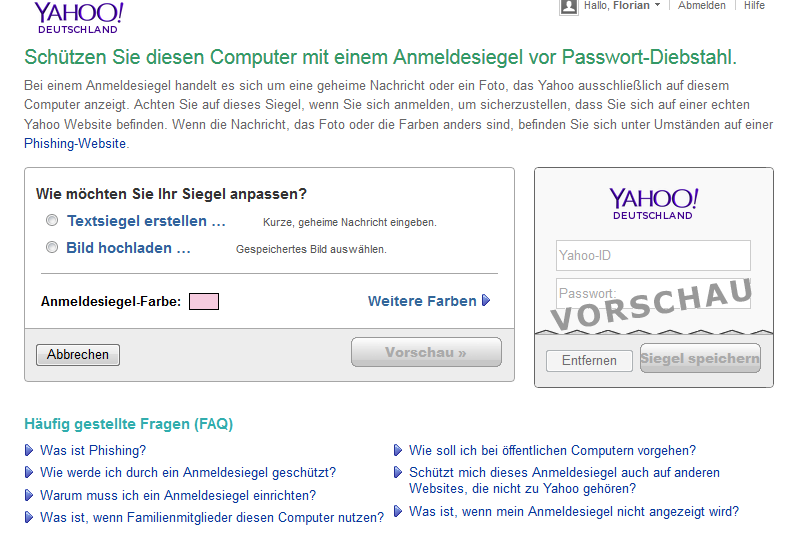
\includegraphics[width=0.5\textwidth]{images/yahoo_anmeldesiegel.png}
							\caption {Sicherheitsniveaus}
							\label{fig:Yahoo_Anmeldesiegel}	
						\end{wrapfigure}
			In Bezug auf das Bereitstellen von Sicherheits-Zusatzfunktionen können die internationalen Mail-Anbieter etwas Punkten. Alle bieten eine 2-Faktor Authentifizierung an. Außerdem hat der Nutzer die Möglichkeit sich eine Liste mit jeglichen externen Anwendung und Webseiten anzeigen zu lassen. Mit dieser erhält er einen Überblick darüber, welche App Zugriff auf welche Nutzerdaten hat.
			Yahoomail kann zusätzlich mit einer Wegwerfadresse, einem Anmeldesiegel (vgl. Abbildung \ref{fig:Yahoo_Anmeldesiegel}) sowie dem selbst entwickelten \ac{DKIM} Verfahren überzeugen. \ac{DKIM} basiert auf asymmetrischer Kommunikation und stellt die Authentizität von E-Mail Absendern sicher.\footcite[Vgl.][]{DKIM}.
			
			
			
%			\begin{wrapfigure}{r}{0.8\textwidth} %wrapfigure ist eine Umgebung, in dem eine Abbildung von TExt umgeben werden kann; {r} steht für rechts, {l} geht auch; zweites Argument ist die Breite des "Einfügekastens"
%							\vspace{-16pt}
%							\centering
%							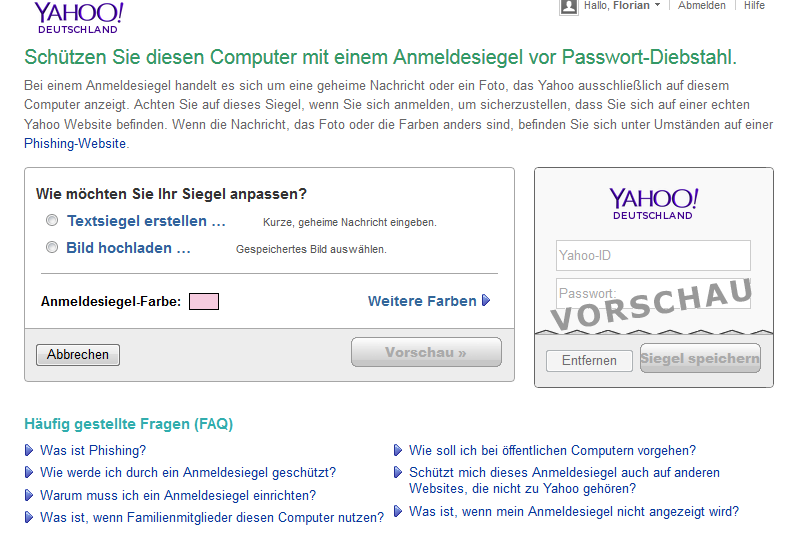
\includegraphics[width=0.6\textwidth]{images/yahoo_anmeldesiegel.png}
%							\caption[Yahoo Anmeldesiegel]{Yahoo: Anmeldesiegel} 
%							\label{fig:Yahoo_Anmeldeseigel} %für "\prettyref"s
%							\vspace{-16pt}
%			\end{wrapfigure} 
			\medskip
			
			Um das Vertrauen der Nutzer in die Provider wieder zu stärken, veröffentlichen Yahoomail und Googlemail  so genannte Transparenzberichte.\footcite[Vgl.][]{Lokshin} In diesen wird dargestellt, welche Behörden welche Art von Auskunft bei den Providern ersucht haben. Microsoft folgt dem Trend und hat bereits angekündigt, die Behördenanfragen für seinen E-Mail Dienst in den Transparenzbericht des Konzerns mit aufzunehmen\footcite[Vgl.][]{Herget}.
			\medskip			
		
		%Links verwendet
						%http://www.heise.de/ix/meldung/Google-experimentiert-mit-End-to-End-Verschluesselung-fuer-GMail-2215680.html
						%http://www.heise.de/mac-and-i/meldung/Auch-Apple-Google-und-Yahoo-wollen-in-E-Mails-schauen-2152971.html
						%http://www.rtl.de/rtl-nachrichtenarchiv/1563673/spitzel-affaere-in-den-usa-microsoft-laesst-nsa-in-outlook-mails-schnueffeln.html
						%https://mailbox.org/microsoft-liest-e-mails-seiner-hotmail-nutzer/
		
		%Links (Backup)
						%http://windows.microsoft.com/de-de/windows/answers?tId=8d16e8b8-d565-4923-bd68-59dbe32aaf4d
						%http://www.patshaping.de/hilfen_ta/pop3_smtp.htm			
						%http://www.heise.de/security/meldung/Yahoo-verschluesselt-jetzt-fast-alles-2161810.html
						%http://www.heise.de/security/meldung/Schutz-fuer-E-Mails-Kleine-Mail-Dienste-ueberzeugen-2098281.html
						
		
			
			\subsection{EmiG - E-Mail made in Germany}
			\ac{EmiG} ist eine Initiative der größten deutschen E-Mail Provider GMX, web.de und T-Online, die zusammen über 53\% (Stand: 2013) der aktiven E-Mail-Konten in Deutschland betreiben.
			\footcite[Vgl.][]{Brandt13} 
			Zusammen mit den Teilnehmern der freenet AG, 1\&1 Internet AG und STRATO AG\footnote{Die 1\&1 Internet AG ist wie GMX und web.de Teil des United-Internet-Konzern, sowie die STRATO AG eine Tochter des Betreiber von T-Online, der Deutschen Telekom AG ist.} deckt EmiG ca. zwei Drittel der aktiven E-Mail Konten in Deutschland ab.\\
			Das Projekt wurde im August 2013 als Reaktion der damaligen \ac{NSA}-Äffäre ins Leben gerufen und hat das Ziel E-Mails zwischen den teilnehmenden Providern auf dem Transportweg mit \ac{TLS/SSL} verschlüsselt versendet werden.
			Seit April 2014 ist das Projekt umgesetzt.
%			\medskip\\
%			Prinzipiell ist das Verfahren ausgelegt weitere Teilnehmer aufzunehmen.
%			Dabei beschreiben die Provider ihre Mail-Infrastruktur im JSON-Format mit \glqq Domainnamen, IP-Adressen, SSL-Zertifikate und Rollen der beteiligten Server.\grqq
%			\footcite[Vgl.][]{Zivadino14-1}
%			Die Teilnehmer spiegeln diese Infrastrukturlisten untereinander um Manipulationen derselben zu erschweren.\\
%			Ein zugehöriger Dienst prüft ob Syntax, IP-Adressen und Hostnamen auf Übereinstimmung um anschließend die SSL-Zertifikate zu verifizieren, die von einer Deutschen CA ausgestellt worden sein müssen.
%			Die Listen werden anschließend geprüft um im Nachgang an Teilnehmer der Initiative verteilt zu werden. 
%			Neue Teilnehmer müssen durch den TÜV Rheinland zertifiziert worden sein, damit die EmiG Teilnehmer die aktualisierte Infrastrukturliste laden.
%			\footnote{Vgl. ebd.}
			\medskip\\
		%Nutzwertanalyse
			Die Nutzwertanalyse (\prettyref{sec:nwa}) wird im Folgenden zusammenfassend für die Provider der Dienste \textit{GMX}, \textit{web.de} und \textit{T-online} beschrieben. 
			Unterschiede, die sich auch auf die Bewertung auswirken werden explizit beschrieben.
		%NWA - Vertraulichkeit	
		\subsubsection{Vertraulichkeit und Integrität}		
			Bei den Providern der EmiG-Initative ist die Vertraulichkeit durch die TLS-Transport"-verschlüsselung gegeben. 
			Die Transportverschlüsselung ist allerdings nur untereinander garantiert. 
			Die Anwender besitzen keine \ac{TLS}-Garantie wenn E-Mails von oder zu Providern außerhalb des Verbunds gesendet oder empfangen werden.\\

			Die Ergebnisse des \ac{SSL}-Test (\prettyref{sec:nwa}) sind für die drei Provider ähnlich gut. GMX und WEB unterstützen Forward Secrecy mit den meisten Browsern, T-Online hingegen lässt den Schlüsselaustausch für ältere Browser über RC4 zu.
			Für die Anwender die innerhalb der EmiG Initiative E-Mails versenden bzw. empfangen ist die Vertraulichkeit des Kommunikationspartner im Webmailer und Outlook ersichtlich.
			Die Anwender sehen in der Adresszeile die E-Mail-Adresse mit einem grünen Haken versehen, sofern sie im \ac{EmiG}-Verbund sind, und bekommen so visualisiert, das die E-Mail transportverschlüsselt versendet wird. Ein zusätzlicher Gewinn an Benutzerfreundlichkeit.
			\footcite[Vgl.][]{Zivadino14-1}\medskip\\
		%NWA - Integrität
		%\subsubsection{Integrität}	
			Die Integrität der E-Mail-Inhalte sind für \ac{EmiG}-Provider von unterschiedlicher Bedeutung.
			\acf{E2EE} ist mit keinem Webmail-Angebot der Provider möglich.

			\begin{wrapfigure}{r}{0.6\textwidth} %wrapfigure ist eine Umgebung, in dem eine Abbildung von TExt umgeben werden kann; {r} steht für rechts, {l} geht auch; zweites Argument ist die Breite des "Einfügekastens"
				\vspace{-12pt}
				\centering
				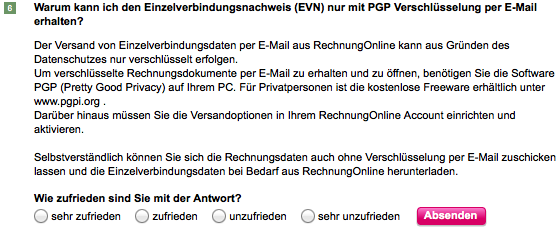
\includegraphics[width=0.6\textwidth]{images/T-Online_Hilfe_PGP}
				\caption[T-Online PGP]{T-Online Hilfe: PGP} 
				\label{fig:T-Online_Hilfe_PGP} %für "\prettyref"s
				\vspace{-12pt}
			\end{wrapfigure}
			Das liegt an einer komplizierten Implementierung und kaum existierender Ansätze für eine Realisierung von PGP im Webmail-Service.
			Im \textit{Hilfe und Support} Bereich von T-Online ist generell keinerlei Hilfe zur Einrichtung von \ac{E2EE} mittels \ac{PGP} oder \ac{S/MIME} zu finden.
			Auch wenn hierfür eine externe Mail-Applikation verwendet werden müsste, könnte technisch versierten Anwendern eine Hilfestellung bei der Einrichtung von \ac{E2EE} bereit gestellt werden.
			Lediglich ein Hinweis über Einzelverbindungsnachweise und weshalb diese nur \ac{PGP}-Verschlüsselt versendet werden dürfen ist zu finden. (\prettyref{fig:T-Online_Hilfe_PGP})
			Eine Information, dass es sich um Ende-zu-Ende-Verschlüsselung handelt ist dem Suchergebnis nicht zu entnehmen.\\
			Die Provider web.de und GMX stellen dem Nutzer eine solche Hilfestellung gut sichtbar in einem eigenen Menüpunkt bereit. (\prettyref{fig:Web-de_Hilfe_PGP})
			Im Angebot von T-Online wird dem Nutzer, aufgrund fehlender \ac{PGP}-Unterstützung, bei der Signierung von E-Mails in externen Mailanwendungen nicht geholfen. 
			Web.de und GMX helfen zwar bei der Einrichtung von \ac{PGP}, weisen jedoch nicht darauf hin, dass durch den Einsatz von \ac{PGP} und E-Mail-Signierung auch die Authentizität des Empfänger und Sender ohne Verschlüsselung sichergestellt werden kann. \\
			
			\begin{wrapfigure}{r}{0.6\textwidth} %wrapfigure ist eine Umgebung, in dem eine Abbildung von TExt umgeben werden kann; {r} steht für rechts, {l} geht auch; zweites Argument ist die Breite des "Einfügekastens"
				\vspace{-12pt}
				\centering
				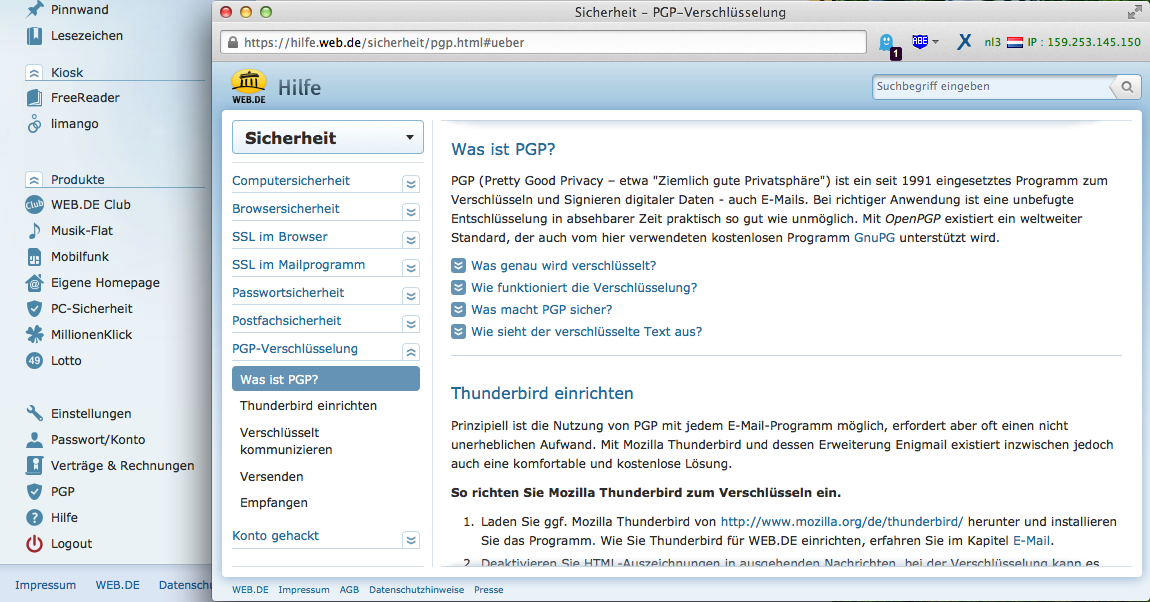
\includegraphics[width=0.6\textwidth]{images/Web-de_Hilfe_PGP}
				\caption[Web.de PGP]{Web.de Hilfe: PGP} 
				\label{fig:Web-de_Hilfe_PGP} %für "\prettyref"s
				\vspace{-24pt}
			\end{wrapfigure}
			Generell haben die Provider der United Internet Gruppe eine informative Sicherheits-Hilferubrik.
			Anwendern wird bei der Einrichtung von \ac{PGP} in der Mailapplikation Thunderbird aktiv unterstützt.
			Für die Applikationen Microsoft Outlook oder Mail.app für Mac besteht jedoch keine Hilfestellung.
			Auch eine Begründung hierfür ist nicht zu finden.
		%NWA - Authentizität
		\subsubsection{Authentizität}
		\label{subsubsec:emig-auth}	
			Die Serverseitige Authentizität der wird mittels dem selbst entwickelten, proprietären Verfahren \textit{\ac{IMPT}} sichergestellt. 
			Dabei prüfen die Mail-Server der Teilnehmer beim Mail-Versand und -Empfang die Client- und Server-Zertifikate gegen die herausgebende \ac{CA}, sowie gegen die Infrastrukturlisten.
			Sollten dabei Inkonsistenzen auftreten wird der Versand abgelehnt.\\
			Dieses Vorgehen erinnert an ein geschlossene Variante von \ac{DANE} (\prettyref{subsec:dane}), welches ähnlich zur Sicherstellung der Authentizität verfährt.
			Alle Partner der Initiative setzen \ac{PFS} ein
			\footcite[Vgl.][]{Zivadino14-1}
			und damit eine Eigenschaft um einem höheren Schutzbedarf in zu entsprechen.
			\footcite[Vgl.][]{Zivadino14-2} 
			\medskip\\
			Der Verzicht auf den offenen Standard \ac{DANE} als Standard-Instrument zur Sicherstellung der Authentizität hat gewiss Nachteile für die Nutzer. 
			Mit \acl{IMPT} existiert jedoch für den E-Mail-Versand unter den \ac{EmiG}-Partnern ein ähnlicher Schutz, der allerdings auch nicht immer die Authentizität der verwendeten \ac{SSL}-Zertifikate gewährleisten kann.
			\footcite[Vgl.][]{Zivadino14-1}
			Die Vorgehensweise zur Entwicklung einer proprietären Lösung ist daher durchaus kritisch zu Hinterfragen. 
			United Internet möchte ggf. den Einsatz von \ac{DNSSEC} und \ac{DANE} in einem Review-Prozess einer Neubewertung unterziehen.
			\footcite[Vgl.][]{Zivadino14-2}
		%NWA - Zusätzliche Sicherheitsrelevante Aspekte
		\subsubsection{Sicherheitsrelevante Aspekte}
			Für die Mails auf den \ac{EmiG}-Servern der \ac{EmiG}-Provider besteht keine separate verschlüsselte Speicherung der E-Mails, insofern dies durch den Nutzer nicht selbst geschehen ist. (\prettyref{subsec:pgp})
			Festplatten werden nicht verschlüsselt um bei Diebstahl oder Beschlagnahmung das Auslesen der Inhalte zu verhindern.
			E-Mails sind für Administratoren der Provider, als auch eventuell unberechtigte Dritte, die sich Zugang auf den Servern verschafft haben einsehbar.\\
			Die Mails werden durch Viren-Scanner, Spam-Filter und wahrscheinlich Analyse-Algorithmen untersucht und ausgewertet.\footcite[Vgl.][]{Kurz13}
			Dazu stimmt der Nutzer den entsprechenden Datenschutz Passagen in den AGBs zu. Diese gewähren den Anbietern das \glqq [\dots] persönliche Daten [\dots] elektronisch verarbeitet werden, [und der Anbieter berechtigt ist] anonymisierte Nutzerinformationen Dritten - darunter Anzeigekunden - [\dots] zur Verfügung zu stellen. Die anonymisierten Daten dürfen [\dots] zur Erstellung von Statistiken und Trenderkennungen sowie zur Qualitätssicherung und Marktforschung verwendet werden.\grqq \footcite[Vgl.][]{Web2012}\\
			Sicherheitsbezogene Informationen sind innerhalb des Webmail-Angebote von United Internet gut auffindbar, könnten allerdings weiterführende Informationen und Anleitungen enthalten.
			T-Online ist beim Angebot von Informationen bzgl. E-Mailsicherheit für eigene Kunden deutlich ausbaufähig.\\
			Einen kleinen Vorsprung besitzt T-Online gegenüber United Internet beim Versuch einen Transparenzbericht zu veröffentlichen, der Anfragen von Behörden offenlegen soll.
			Allerdings ist der Transparenzbericht ein halbherziger Versuch offener, transparenter Kommunikation, denn  die exakte Anzahl der Verkehrsdatensätze bleibt weiterhin unklar.
			\footcite[Vgl.][]{Beuth14}
			United Internet erarbeitet derzeit noch an einem Modell, um Transparenz zu schaffen.
			\footcite[Vgl.][]{Boehm14}
		%Zusammenfassung
		\subsubsection{Zusammenfassung}
			\ac{EmiG} ist im Prinzip ein deutlicher Gewinn an Sicherheit für die Kunden im Vergleich zur Zeit vor dem Projekt. 
			Mit Rückblick auf die Zeit vor der Initiative und dem damalig gebotenen Sicherheitsniveau im Jahre 2013 ist dieser Gewinn an Sicherheit jedoch kein stark herausragendes Merkmal.
			Höher als Sicherheitsniveau-Stufe 2 ist die E-Mail-Kommunikation nicht zu bewerten, die auch erst seit dem \ac{TLS}-Verbund erreicht wird.\footnote{Zum Vergleich: 2013 war Stufe 1 das maximale Sicherheitsniveau für Anwender der größten E-Mail-Provider Deutschlands.}
			Dafür fehlen weiterhin Provider-übergreifende Bemühungen interessierten Anwendern die \ac{E2EE} näher zu bringen.
			Es könnte durchaus mehr Energie in die Umsetzung von \ac{E2EE} im Webmailer aufgewendet werden, wie es im Vergleich zu anderen Anbietern geschieht (Vgl. \prettyref{subsubsec:googlemail} und \prettyref{subsubsec:mailbox}) \medskip\\
			Vor allem der Entschluss zur Insellösung \ac{IMPT} und Vernachlässigung von Standards wie \ac{DNSSEC} werfen Fragen auf. 
			Ob \ac{DANE} tatsächlich eine Chance auf eine spätere Implementierung bekommt bleibt abzuwarten, denn bisher ist mit \ac{IMPT} die Kommunikation mit internationalen Anbieter und garantierter Transportverschlüsselung rhetorisch ausgeschlossen.
			\footcite[Vgl.][]{Zivadino14-1}
			Fakt ist bisher das die Aufnahme und Erstzertifizierung neuer Mail-Provider, die am Beitritt der Initiative interessiert sind, Kosten in Höhe von 9.500 bis 30.000 Euro
			\footcite[Vgl.][]{Zivadino14-3} 
			verursacht und mit zusätzlichen manuellen Aufwand bei der Konfiguration der \ac{SMTP}-Mailserver verbunden sind.
			Daher wächst die Initiative nur langsam.\\
			Auch Vorwürfe, dass \ac{EmiG} scheinbar keine kleineren E-Mail-Provider zulassen möchte wurden veröffentlicht.
			\footcite[Vgl.][]{Zivadino14-4}
			Ob \ac{EmiG} tatsächlich ein offener Verbund ist, oder sich nur als solcher verkauft bleibt zur Zeit auch unbeantwortet. \medskip\\
			Inwieweit die Initiative letztendlich die Hauptaufgabe hat Anwendern ein deutliches Plus an Sicherheit zu gewährleisten werden erst die nächsten Monate zeigen können.
			Die geplante Einreichung der Initiative, das eigens entwickelte Verfahren als \ac{RFC} beim \ac{IETF} \glqq (...), dem für Internet-Standards verantwortlichem Gremium, (...)\grqq\footcite[Vgl.][]{Zivadino14-2}
			standardisieren zu lassen ist der richtige Weg zur Beantwortung vieler Fragen.
			Ob andere E-Mail-Provider diesen Standard nutzen werden, wenn man zusätzliche Kosten und Aufwand betrachtet, bleibt abzuwarten. Auch die Kompatibilität zwischen \ac{DNSSEC} und \ac{IMPT} kann ein Entscheidungskriterium sein.
			\medskip\\
			Bisher betreibt \ac{EmiG} einen hohen Marketingaufwand mit breitangelegter TV Kampagne und dazugehörigen, typisch unklaren Äußerungen, hinter denen vermutlich auch strategisch, politische Interessen der Anbieter liegen.\\
			Die Haltung, Anwender auf der Internetseite\footnote{\url{http://www.e-mail-made-in-germany.de/Verschluesselung.html}} 
			nicht über alle Sicherheitsaspekte zu informieren und im Werbespot\footnote{\url{http://www.e-mail-made-in-germany.de/Wechseln.html}} den Großteil technisch nicht versierter Anwender in falscher Sicherheit wiegt hinterlässt ebenfalls Fragen.
			Für eine sichere und Provider-unabhängige E-Mail-Kommunikation sollte es im Informationszeitalter nicht 15 Jahre für den Einsatz von Sicherheitsstandards benötigen.
			Ob \ac{EmiG} sich nur als offener Verbund verkauft oder tatsächlich ist, wird gleichermaßen in den nächsten Monaten zuverlässiger beantwortet werden können.
			
%			Kritisch zu betrachten ist, dass die Umsetzung der Transportverschlüsselung 15 Jahre seit Verabschiedung des Standards 1999 und eine Datenschutzaffäre noch unabschätzbaren Ausmaßes benötigt, um von den größten E-Mail Providern Deutschlands obligatorisch und verantwortungsvoll umgesetzt zu werden. 
%			Konkurrent Google unterstützt bspw. beim eigenen E-Mail Dienst seit 2011 durch PFS.\footcite[Vgl.][]{Boeck2013}
%			
%			\begin{wrapfigure}{r}{0.5\textwidth} %wrapfigure ist eine Umgebung, in dem eine Abbildung von TExt umgeben werden kann; {r} steht für rechts, {l} geht auch; zweites Argument ist die Breite des "Einfügekastens"
%				\vspace{-24pt}
%				\centering
%				\begin{itemize}
%					\renewcommand{\labelitemi}{$\Rightarrow$}
%					\item smtp\_use\_tls=yes
%					\item smtpd\_use\_tls=yes
%				\end{itemize}
%				\caption[EmiG: SSL/TLS wurde aktiviert]{E-Mail-Server Einrichtung von obligatorischem SSL/TLS\footnotemark}
%				\label{fig:emig_tls} %für "\prettyref"s
%				\vspace{-12pt}
%			\end{wrapfigure}\footnotetext{\cite[In Anlehnung an][S. 9]{Rundfeldt14}}
%			Ferner wird der Aufwand der Einstellung als sehr gering Eingeschätzt. (\prettyref{fig:emig_tls})\\
%			Zertifikate müssen für Teilnehmer der Provider von deutschen \acp{CA} ausgestellt sein.\medskip\\	

			\subsection{Alternative Provider}
			Als alternative Provider werden zwei kleine Anbieter, die bereits aktiv am Markt sind, untersucht.
			Hierbei handelt es sich um die beiden in Berlin ansässigen Provider \textit{Posteo} und \textit{mailbox.org}.
			Diese Anbieter positionieren sich bewusst im Kontrast zu den großen Mailprovidern als Alternativen, die einen hohen Wert auf die Privatsphäre ihrer Kunden legen und daher möglichst wenig Daten ihrer Nutzer protokollieren und die Mails der Nutzer nicht auswerten.\footcite[Vgl.][]{Posteo2013a, Mailbox2014}
			
				\subsubsection{posteo}
				\label{subsubsec:posteo}
					Posteo ist ein kleiner, deutscher Mailprovider, der 2009 gegründet wurde und von der Posteo e.K. betrieben wird. \footcite[Vgl.][]{Posteo2013b}
					Laut eigenen Angaben verzeichnet das Unternehmen einen Nutzerzuwachs um mehr als 100\% pro Jahr.\footcite[Vgl.][]{Posteo2013b}
					Er probiert sich bewusst von den Konkurrenten abzusetzen durch das Angebot von innovativen Sicherheitsfunktionen und die garantierte Werbefreiheit.
					Die Kosten deckt Posteo dadurch, dass für die Nutzung des Dienstes eine monatliche Gebühr erhoben wird.
					Diese kann auf unterschiedliche Weise bezahlt werden und kann durch die Löschung der Beziehungsdaten zwischen Zahlungseingang und Postfach nach erfolgter Zahlung nciht zurückverfolgt werden.
					Dadurch soll eine anonyme Nutzung des Postfachs ermöglicht werden, da auch bei der Registrierung keine persönlichen Daten angegeben werden müssen.\footcite[Vgl.][]{Posteo2013a}
					Nachfolgend wird die durchgeführte Nutzwertanalyse für Posteo beschrieben.
					\medskip\\
					
					\paragraph{Vertraulichkeit und Integrität}
						Der Zugriff auf den Server von Posteo erfolgt immer über eine mit \ac{TLS} und \ac{PFS} gesicherte Verbindung, unabhängig davon, ob ein Mailprogramm oder der Webmailer genutzt wird.
						Dies wird durch den Einsatz von \ac{HSTS} erzwungen.
						Beim eigentlichen Versand und Empfang von Mails geht Posteo jedoch nicht ganz so strikt vor und nutzt eine verschlüsselte Verbindung lediglich, wenn dies durch den Kommunikationspartner ebenfalls unterstützt wird.
						Das Zertifikat, dass Posteo bei der Transportverschlüsselung einsetzt, ist ein sogenanntes erweitertes Zertifikat, das es dem Anwender auf einen Blick ermöglichen soll den Betreiber der aufgerufenen Webseite bzw. des Servers zu identifizieren.\footcite[Vgl.][]{Posteo2013c}\medskip\\
					
						Im Webmailer ist es momentan nicht möglich, die Mails mittels \ac{E2EE} zu versendenet aber die sichere Speicherung des privaten Schlüssels des Nutzers noch Probleme, so dass nicht feststeht zu welchem Zeitpunkt diese Funktion zur Verfügung stehen wird.\footcite[Vgl.][]{Posteo2013c}
						Über die Verschlüsselungsmöglichkeiten per \ac{PGP} und \ac{S/MIME} und die damit verbundenen Vor- und Nachteile in Bezug auf anonyme Kommunikation wird auf der Webseite von Posteo ausführlich informiert.
						Eine konkrete Hilfestellung zur Einrichtung der Verschlüsselungsverfahren zur Nutzung mit einem Mailprogramm wird bisher nicht gegeben.
						Stattdessen wird auf die Seite von \textit{Netzpolitik.org}\footnote{\url{https://netzpolitik.org/2013/anleitung-so-verschlusselt-ihr-eure-e-mails-mit-pgp}} und dem Mailprogramm \textit{Thunderbird} der Mozilla Foundation\footnote{\url{http://www.thunderbird-mail.de/wiki/Mailverschlüsselung_mit_S/MIME}} verlinkt.
					
					\paragraph{Authentizität}
						Auf die Möglichkeiten, die Mails vor dem Versand digital zu signieren und wie dies im Mailprogramm durchgeführt werden kann, werden auf der Posteo-Seite ein paar Informationen gegeben.
						Eine Anleitung, wie das Signieren durchgeführt wird sucht der Nutzer allerdings vergeblich.
						Auch die Tatsache, dass eine Verschlüsselung im Webmailer bisher nicht möglich ist, lässt darauf schließen, dass ebenfalls keine Signaturen erstellt werden können.
						Eine direkte Information hierzu gibt es aber nicht.
						Bei der Authentifizierung ihrer Server ist Posteo jedoch hochaktuell und hat als einer der ersten\footnote{Auch Mailbox.org setzt seit Mai 2014 \ac{DANE} ein(\cite[Vgl.][]{Mailbox2014a}), so dass nicht zweifelsfrei belegt werden kann, wer diese Funktion zuerst genutzt hat.} Anbieter in Deutschland \ac{DANE} umgesetzt.\footcite[Vgl.][]{Zivadino14-5}\medskip\\
					
					\paragraph{Zusätzliche sicherheitsrelevante Aspekte}
						Im Bereich der zusätzlichen sicherheitsrelevanten Aspekte kann Posteo durch die Verschlüsselung seiner Festplatten mit \ac{AES} punkten.
						Hierdurch sind die gespeicherten Mails vor Zugriffen geschützt, falls die Festplatten geklaut oder beschlagnahmt werden sollten.
						Die Mails selbst werden jedoch nicht extra verschlüsselt gespeichert, wodurch sie für Personen, die sich unberechtigten Zugriff auf die Server im laufenden Betrieb verschaffen können, auslesbar sind.
						Die Möglichkeit für eine zusätzliche Verschlüsselung der Mails ist jedoch ebenfalls für die Zukunft geplant.\footcite[Vgl.][]{Posteo2013c}
						Insgesamt wäre es wünschenswert, wenn Posteo bei dem geäußerten Anspruch auf hohen Datenschutz und Wahrung der Privatspähre seiner Nutzer, diesen gut verständliche Anleitungen für die Einrichtung und Nutzung von Verschlüsselungsverfahren und digitalen Signaturen geben würde.
						Wie bereits zu Beginn der Ausführungen zu den alternativen Providern erwähnt garantiert Posteo seinen Nutzern Werbefreiheit.
						Aus diesem Grund werden die Mails weder beim Versand noch beim Empfang durch Posteo analysiert.
						Eine weitere Sicherheitsfunktion ist das sogenannte \ac{IP}-Stripping.
						Hierbei wird die \ac{IP}-Adresse des Absenders durch die \ac{IP}-Adresse des Mailservers von Posteo ersetzt.
						Somit ist eine Rückverfolgung zum Absender aufgrund der \ac{IP}-Adresse nicht möglich.\footcite[Vgl.][]{Posteo2013a}
						Auch was die Veröffentlichung eines Transparenzberichts angeht ist Posteo vorbildlich und hat als erster deutscher Anbieter diesen veröffentlicht und damit die großen Konkurrenten wie beispielsweise die \ac{DTAG} als Betreiber von T-Online unter Zugzwang gesetzt.
					
					
				\subsubsection{mailbox.org}
				\label{subsubsec:mailbox}
					Mailbox.org startete im Februar 2014 als neuer E-Maildienst der Heinlein Support GmbH, die mit JPBerlin bereits seit über 20 Jahren als \ac{ISP} auftritt und E-Mailpostfächer anbietet.
					Die Abgrenzung zur Konkurrenz erfolgt, wie auch bei Posteo, über die explizite Betonung des Datenschutzes und der Privatsphäre des Kunden.
					Dies ist unter anderem am Werbespruch zu erkennen, der \glqq damit Privates privat bleibt\grqq{} lautet.
					Auch bei Mailbox.org gibt es kein kostenloses Angebot zur Nutzung des E-Maildienstes, dafür aber ebenso das Versprechen von Werbe- und insbesondere auch hohem Spamschutz.\footcite[Vgl.][]{Mailbox2014}
					In den folgenden Abschnitten wird die Durchführung der Nutzwertanalyse für Mailbox.org beschrieben.
					
					\paragraph{Vertraulichkeit und Integrität}
						Bei Mailbox.org können die Nutzer nur auf verschlüsseltem Weg auf die Server zugreifen um ihre Mails abzurufen.
						Hierbei werden die neuesten Versionen von \ac{TLS} mit \ac{PFS} unterstützt und der Aufbau von unverschlüsselten Verbindungen durch den Einsatz von \ac{HSTS} unterbunden.
						Auch beim Versand und Empfang von Mails bietet Mailbox.org die Möglichkeit eine unverschlüsselte Kommunikation zu unterbinden.\footcite[Vgl.][]{Mailbox2014b}\medskip\\
						
						Bei der Information der Nutzer über die Einrichtung und Nutzung von Verschlüsselungsmethoden zur \ac{E2EE} bietet Mailbox.org eine Anleitung für viele Plattformen und auch einen gut verständlichen Stiftfilm zur Erklärung, wie \ac{E2EE} funktioniert.
						Eine Nutzung der \ac{E2EE} im Webmailer ist aber wie bei den anderen Providern nicht möglich.
						
					\paragraph{Authentizität}
						Zur Authentifizierung seiner Mailserver setzt Mailbox.org \ac{DANE} ein und unterstreicht hiermit seinen Anspruch als Anbieter für die sichere Kommunikation per E-Mail.
						Aus dem gleichen Grund scheint es selbstverständlich, dass Mailbox.org ebenfalls Informationen zu den Möglichkeiten der digitalen Signatur vermittelt.
						Doch auch hier wäre eine genauere Anleitung zur Nutzung dieser wünschenswert um diese technische Maßnahme für die Nutzer einfach einsetzbar zu machen.
						Dazu würde auch eine Implementierung dieser Funktion im Webmailer gehören.
						Hierzu sind aber auf der Website des Mailproviders keine Angaben zu finden, ob eine Umsetzung geplant ist.
						
					\paragraph{Zusätzliche sicherheitsrelevante Aspekte}
						Mit dem Möglichkeit der Zweifaktorauthentifizierung mit einem \ac{OTP} hebt sich Mailbox.org ebenfalls von vielen Konkurrenten ab.
						Zur Nutzung dieser Funktion muss ein USB-Gerät, ein sogenannter Yubikey, mit dem Account verbunden werden.
						Dadurch ist es möglich, sich auch von unbekannten und damit potenziell unsicheren Rechner sicher an seinem Account im Webfrontend anzumelden.
						Ebenfalls positiv hervorzuheben ist die regelmäßige Berichterstattung über Probleme und Erweiterungen des Funktionsumfangs, auch gerade im Hinblick auf neu eingeführte Sicherheitsmaßnahmen.
						
%				\subsubsection{Zusammenfassung}
					
					
			\subsection{De-Mail}
			
			=====COMMENT
			
			Absprache Keyserver bei De-Mail
			
			=====COMMENT END
			
			Seitdem am 3. Mai 2011 das De-Mail-Gesetz in Kraft getreten ist, können die darauf basierenden De-Mail-Dienste genutzt werden.
			Das ursprünglich unter dem Projektnamen \glqq Bürgerportale\grqq entwickelte Konzept hat zum Ziel, eine elektronische und rechtlich verbindliche Kommunikation zu ermöglichen.
			Dadurch werden die Vorteile der {\textit{\glqq Schnelligkeit der E-Mail in Verbindung mit der Sicherheit eines Briefes und der Nachweis eines Einschreibens\grqq}\footcite[Vgl.][S. 8]{BSIDeMail} genutzt.
			Obwohl die Nutzung von De-Mail nicht komplizierter als die Nutzung herkömmlicher E-Mails ist, sind beide Kommunikationsmittel nicht interoperabel, d. h. De-Mail-Nachrichten können nicht als herkömmliche E-Mails empfangen und versendet werden und umgekehrt.
			De-Mail-Nachrichten können jedoch Empfängern anderer De-Mail-Anbieter verschickt werden.
			Die per De-Mail verschickten Nachrichten bleiben im Verbund der De-Mail-Provider.
			Um als De-Mail-Anbieter akkreditiert zu werden, müssen künftige De-Mail-Anbieter sich eine Reihe von Sicherheitsanforderungen erfüllen und einen Prüfungsprozess absolvieren.
			Nach erfolgreicher Prüfung werden die Anbieter durch das \ac{BSI} akkreditiert.\medskip\\
			
			Um sich in das De-Mail-Konto anzumelden gibt es grundsätzlich zwei verschiedene Anmeldeverfahren.
			In der Stufe \glqq normal\grqq meldet sich der Nutzer mit seinem Benutzernamen und Passwort an.
			Meldet sich der Nutzer im \glqq hohen\grqq Sicherheitsmodus an, wird zusätzlich zum Benutzernamen und Passwort ein sogenannter Token benötigt.
			Bei dieser sogenannten Zwei-Faktor-Authentifizierung wird der Anmeldevorgang durch einen Gegenstand, der im Besitz des Nutzers ist, zusätzlich gesichert.
			Abhängig von dem Anmeldeverfahren können verschiedene Versandoptionen genutzt werden:
			
			\begin{itemize}
				\item Versandbestätigung: Bei Wahl dieser Option wird eine Versandbestätigung vom Versanddienst des Absenders erzeugt und dem Absender per Nachricht zugestellt.
				\item Eingangsbestätigung: Bei Wahl dieser Option wird eine Zugangsbestätigung vom Postfachdienst des Empfängers erzeugt und dem Absender sowie dem Empfänger der ursprünglichen Nachricht per Nachricht zugestellt.
				\item Persönlich: Die Wahl dieser Option bedeutet, dass das erforderliche Anmeldeniveau des Empfängers mindestens "hoch" sein muss, um die Nachricht lesen zu können. Um diese Option wählen zu können, muss auch das Anmeldeniveau des Absenders "hoch" sein.
				\item Absender-bestätigt: Mit der Wahl dieser Option bringt der Absender zum Ausdruck, dass er sich verbindlich an den von ihm versendeten Nachrichteninhalt gebunden fühlt. Um diese Option wählen zu können, muss das Anmeldeniveau des Absenders "hoch" sein. Der Empfänger erfährt, dass der Absender beim Versand der Nachricht "hoch" angemeldet war.\footcite[Vgl.][]{BSIMerkmale}
			\end{itemize}
			Bei den ersten beiden Optionen \textit{\glqq sendet der De-Mail-Anbieter Ihnen [den Nutzer, Anm. der Autoren] eine qualifiziert elektronisch signierte Bestätigung darüber, wann und an wen Sie die De-Mail verschickt haben bzw. wann die Nachricht im Postfach des Empfängers einging\grqq}. \footcite[Vgl.][S. 15]{BSIDeMail}\medskip\\
			
			Die derzeit bekannteren De-Mail Diensteanbieter sind die Telekom mit Ihrem eigenen Mailservice und die United Internet AG mit 1\&1, web.de und gmx.de.
			Weitere Diensteanbieter sind die Mentana-Claimsoft GmbH sowie die T-Systems International GmbH \footcite[Vgl.][]{BSIDiensteanbieter}.\medskip\\
			
			Die drei Sicherheitsaspekte Vertraulichkeit, Integrität und Authentizität sind im Umgang mit De-Mail wesentlich \footcite[Vgl.][]{BSIGrundlagen}.
			Im Folgenden werden diese drei Aspekte im Zusammenhang mit De-Mail näher untersucht.
			
			Bevor De-Mail genutzt werden kann, wird ein De-Mail-Konto mit einer De-Mail-Adresse benötigt, nach dessen Registrierung eine Identifikation notwendig ist.
			Die Überprüfung der Identität erfolgt beim De-Mail-Anbieter.
			Der Nutzer muss sich dabei mit einem gültigen Ausweisdokument identifizieren lassen.
			Auch eine Identifizierung über die \textit{\glqq Online-Ausweisfunktion (eID-Funktion) im neuen Personalausweis (nPA)\grqq} \footcite[Vgl.][S. 13]{BSIDeMail} ist möglich.
			Dieses Verfahren dient dazu, die Authentizität des Nutzers festzustellen.\medskip\\
			
			De-Mails werden auf dem ganzen Transportweg verschlüsselt übertragen, um die Mail vor unberechtigten Zugriff zu schützen.
			Auf dem Transportweg liegt die De-Mail für einen kurzen Zeitabschnitt unverschlüsselt vor, wenn sie den De-Mail-Anbieter erreicht. \footcite[Vgl.][S. 16]{BSIDeMail} 
			In diesem Moment wird die De-Mail auf Schadsoftware untersucht. Sollte die De-Mail Schadsoftware enthalten, wird der Empfänger beim Erhalt der Nachricht davor gewarnt.
			Im Vergleich zur herkömmlichen Mail-Verschlüsselung werden auch die Metadaten verschlüsselt. \footcite[Vgl.][]{BSIMerkmale}
			Darüber hinaus existiert die Möglichkeit, eine End-to-End-Verschlüsselung zu nutzen.
			Dabei müssen beide Kommunikationsteilnehmer eine separate Verschlüsselungssoftware verwenden. Durch diese zusätzliche Maßnahme sind auch die De-Mail-Anbieter nicht in der Lage, die Nachrichten zur Schadsoftware-Überprüfung kurzzeitig zu entschlüsseln.\medskip\\
			
			Die Integrität einer De-Mail gewährleistet, indem der De-Mail-Anbieter nach Eingang der versendeten Nachricht eine Prüfsummer oder elektronische Signatur erzeugt und diese dem Empfänger übermittelt.
			Die De-Mail kann daher während der Übertragung nicht modifiziert werden, ohne dass der Empfänger es merkt.
			
			\subsubsection{Kritik}
			Linus Neumann vom \ac{CCC} im Jahre 2013 in zwei Stellungnahmen zu Gesetzesvorhaben der Bundesregierung bzgl. der rechtsverbindlichen Kommunikation Kritik gegenüber den gegebenen Anforderungen von De-Mail geäußert.\footcite[Vgl.][]{Neumann2013a,Neumann2013b} %\footcite{Neumann2013b}
			Zum einen sei die Authentizität beim Versenden einer De-Mail-Nachricht nicht immer gegeben. Lediglich einmalig bei der Registrierung wird die Identität des Nutzers überprüft. \footcite[Vgl.][]{Neumann2013b} 
			Beim Versenden erfolge keine weitere Überprüfung der Authentizität.
			Werden die Zugangsdaten abgefangen, hätten Angreifer Zugriff auf das Konto und Nachrichten als vermeintlich rechtmäßigen Absender verschicken.
			Selbst die Anmeldung mittels der Zwei-Faktor-Authentifizierung biete nicht genügend Schutz, da nach einmaliger Anmeldung \textit{\glqq mehrere De-Mails ohne erneute Authentifizierung gesendet werden\grqq} \footcite[Vgl.][o.S.]{Neumann2013b} können.
			Dazu bieten sich Angriffsszenarien wie dem Man-in-the-Middle-Angriff an, um an die Zugangsdaten zu gelangen.\medskip\\
			
			Ein ähnliches Problem ergibt sich im Zusammenhang mit der Integrität einer De-Mail-Nachricht.
			Nach dem Versand der Nachricht wird die De-Mail vom De-Mail-Anbieter signiert.
			Dies garantiert zwar, dass die Nachricht unterwegs nicht verändert wurde.
			Mittels den oben beschriebenen Angriffsszenarien kann der Angreifer eine Nachricht verschicken und der Empfänger geht fälschlicherweise davon aus, dass die Nachricht unverändert wurde. \footcite[Vgl.][o.S.]{Neumann2013b}\medskip\\
			
			Die Vertraulichkeit durch die Verschlüsselung sei zwar gegeben, durch die kurzzeitige explizite Entschlüsslung beim De-Mail-Anbieter sei diese nicht konsistent.\footcite[Vgl.][S. 4]{Neumann2013a}
			Unbefugte hätten theoretisch die Möglichkeit, an den Inhalt der Nachricht zu gelangen.\medskip\\
			
			Laut Neumann sei es noch nicht zu spät für die Nachbesserung des De-Mail-Gesetztes. \footcite[Vgl.][S. 6f]{Neumann2013a}
			Er empfiehlt eine standardmäßige Ende-zu-Ende-Verschlüsslung\footcite[Vgl.][S. 7,o.S.]{Neumann2013a,Neumann2013b} sowie die Einhaltung der Vorgaben des Signaturgesetzes.\footcite[Vgl.][S. 4]{Neumann2013a}
				
			
	\chapter{Fazit und Ausblick}
%		(Trends/Fazit/Schlusswort -> proton Mail Provider vom CERN)
%		(Google hat die alpha eines Plugins für Chromebrowser vorgestellt, die E2E-Verschlüsselung im Browser durchführen und vereinfachen soll -> könnte nen Hinweis wert sein) 	
%		Da das Thema noch aktuell ist, und ständig weiter lebt macht es vll Sinn genau nochmal drauf aufmerksam zu machen das es nur um eine Moment-Aufnahme handelt. 
		\color{black}
		Die Durchführung der Nutzwertanalyse hat gezeigt, dass es große Unterschiede zwischen den Angeboten der Mailprovider hinsichtlich der Umsetzung von Sicherheitsverfahren gibt.
		Den meisten Providern scheinen aber die Sicherheitsprobleme bewusst zu sein und auch die Enthüllungen durch Edward Snowden haben sie veranlasst, die in den Protokollen vorhandenen Sicherheitsverfahren auch einzusetzen.
		Dies wird nicht zuletzt durch die Gründung der \ac{EmiG}-Initiative deutlich.\medskip\\
		
		Trotzdem muss man die in der Nutzwertanalyse festgestellte Situation als Momentaufnahme werten, da in diesem Markt, wie generell im IT-Bereich, sehr viel Bewegung ist.
		Dies lässt sich daran festmachen, dass neben den untersuchten, alternativen Mailprovidern, die in Deutschland ansässig sind, auch weitere Anbieter wie \textit{Protonmail.ch} aus der Schweiz oder \textit{startmail.com} der Suchmaschine \textit{ixquick} demnächst in den Markt eintreten und eine automatische \ac{E2EE} der E-Mails versprechen, ohne dass der Nutzer zusätzliche Software benötigt.\footnote{Vgl. \url{http://www.protonmail.ch} und \url{http://beta.startmail.com}}
		Dadurch soll die Privatsphäre der Nutzer geschützt werden und das Mitlesen von Mails durch unberechtigte Dritte verhindert beziehungsweise erschwert werden.\medskip\\
		
		Doch auch die großen Provider probieren hier nicht in den Anschluss zu verlieren.
		So hat Google bereits eine erste Testversion eines Browser-Addons zur Mailverschlüsselung im Browser veröffentlicht, die eine \ac{E2EE} stark vereinfachen soll.		
		Die Entwicklung in der nächsten Zeit wird zeigen, ob die großen Mailprovider durch die alternativen Provider dazu gezwungen werden, ebenfalls verstärkt Informationen und Unterstützung bei der Verschlüsselung von E-Mails zu bieten oder ob sich das Interesse der Öffentlichkeit für Themen des Datenschutz wieder legen wird.\medskip\\
		
		Insgesamt lässt sich sagen, dass die bisher durchgeführten Schritte der meisten Provider zur Transportverschlüsselung von E-Mails ein Schritt in die richtige Richtung sind, diese den Nutzer jedoch nicht in falscher Sicherheit wiegen dürfen.
		Aufgrund der Tatsache, dass eine \ac{E2EE} momentan noch mit einigen technischen Hürden verbunden ist und einen Komfortverlust, in Bezug auf die Lesbarkeit der Nachrichten auf unterschiedlichen Endgeräten mit sich bringt, ist der Einsatz der E-Mail zur Kommunikation auf der definierten Sicherheitsstufe 4 nur in manchen Fällen geeignet.
		An dieser Stelle muss jeder einzelne Nutzer selbst abwägen, wie wichtig für ihn die übermittelte Information ist und ob er zu deren Schutz die bestehenden Komforteinbußen hinnehmen kann und will.
		
%		
%			- wie aus NWA ersichtlich, gibt es große Unterschiede zwischen den Angeboten der Provider hinsichtlich Sicherheit
%				- den meisten Providern scheinen aber mögliche Sicherheitsprobleme bei der E-Mailkommunikation bewusst zu sein
%				- Entwicklung hin zu standardmäßig mehr Sicherheit durch Initiative wie EmiG erkennbar
%				- nur Momentaufnahme der Situation, denn Markt in Bewegung, da neben großen Providern, die an VEreinfachung der Nutzung von Verschlüsselungsverfahren arbeiten (--> Google mit Browser Addon für Chrome (End-to-End))auch weitere Anbieter in den Markt drängen, die wie Mailbox.org und Posteo den Schutz der Privatsspähre ihrer Kunden in den Vordergrund stellen (--> Protonmail.ch und Startmail)  
%				
%				- trotz Bemühungen der Provider noch Möglichkeiten zur VErbesserung
%				- kritisch sind die Werbemaßnahmen zu betrachten, die den normalen Nutzer ggf. in falscher Sicherheit wiegen (--> s. EmiG-Kampagne: Mail ist sicher da verschlüsselt übertragen...)
%				
%				- Fazit: die verschlüsselte Übertragung von Mails ist besser als nichts, aber eine E2EE ist noch besser
%				- wird vermutlich nicht durch große Provider gefördert, da diese ihr kostenloses Angebot über Werbung finanzieren und zur Personalisierung gerne wissen möchten, worüber ihre Kunden schreiben --> bei E2EE nicht möglich
%				
%				- Snowden-Affäre hat dazu geführt, dass sich mehr Inititiven auf diesem GEbiet ergeben haben
%				- Zielgruppe ist sensibler geworden, was Daten angeht
%				- Abwägen zwischen Sicherheit und Komfort wichtig
%				
%				- zur sicheren Kommunikation ist die E-Mail aus genannten Gründen nicht die erste Wahl
%									
	\chapter*{Literaturverzeichnis}
	\fancyhead{}
	\renewcommand{\headrulewidth}{0pt}	
		\addcontentsline{toc}{chapter}{Literaturverzeichnis}
		%Literaturverzeichnis
		\printbibliography[heading=offline,nottype=online]
		\printbibliography[heading=online,type=online]
	\chapter*{Anhang}\label{sec:anhang}
		\addcontentsline{toc}{chapter}{Anhang}
		\label{LastPage}
		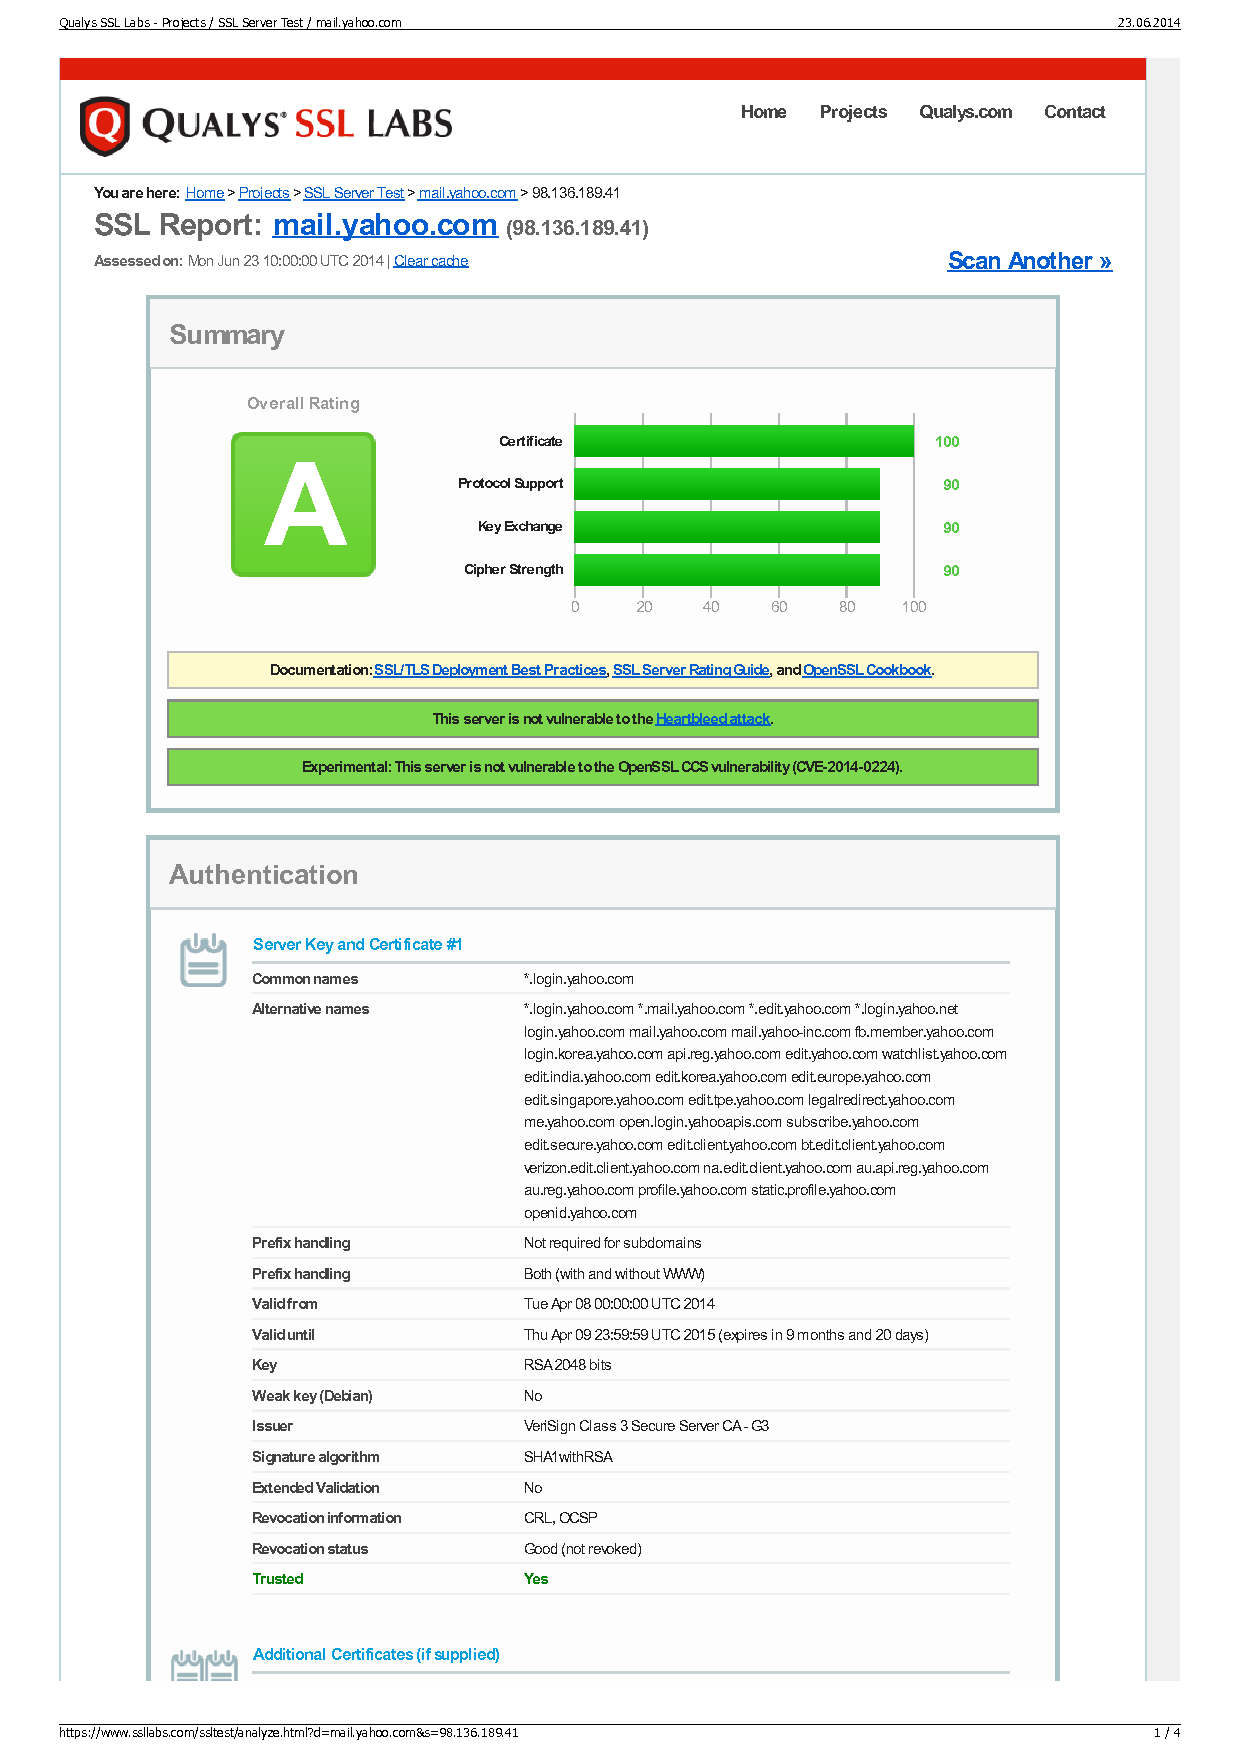
\includepdf[pages=1-4]{anlagen/SSLServerTest-yahoo.pdf}
		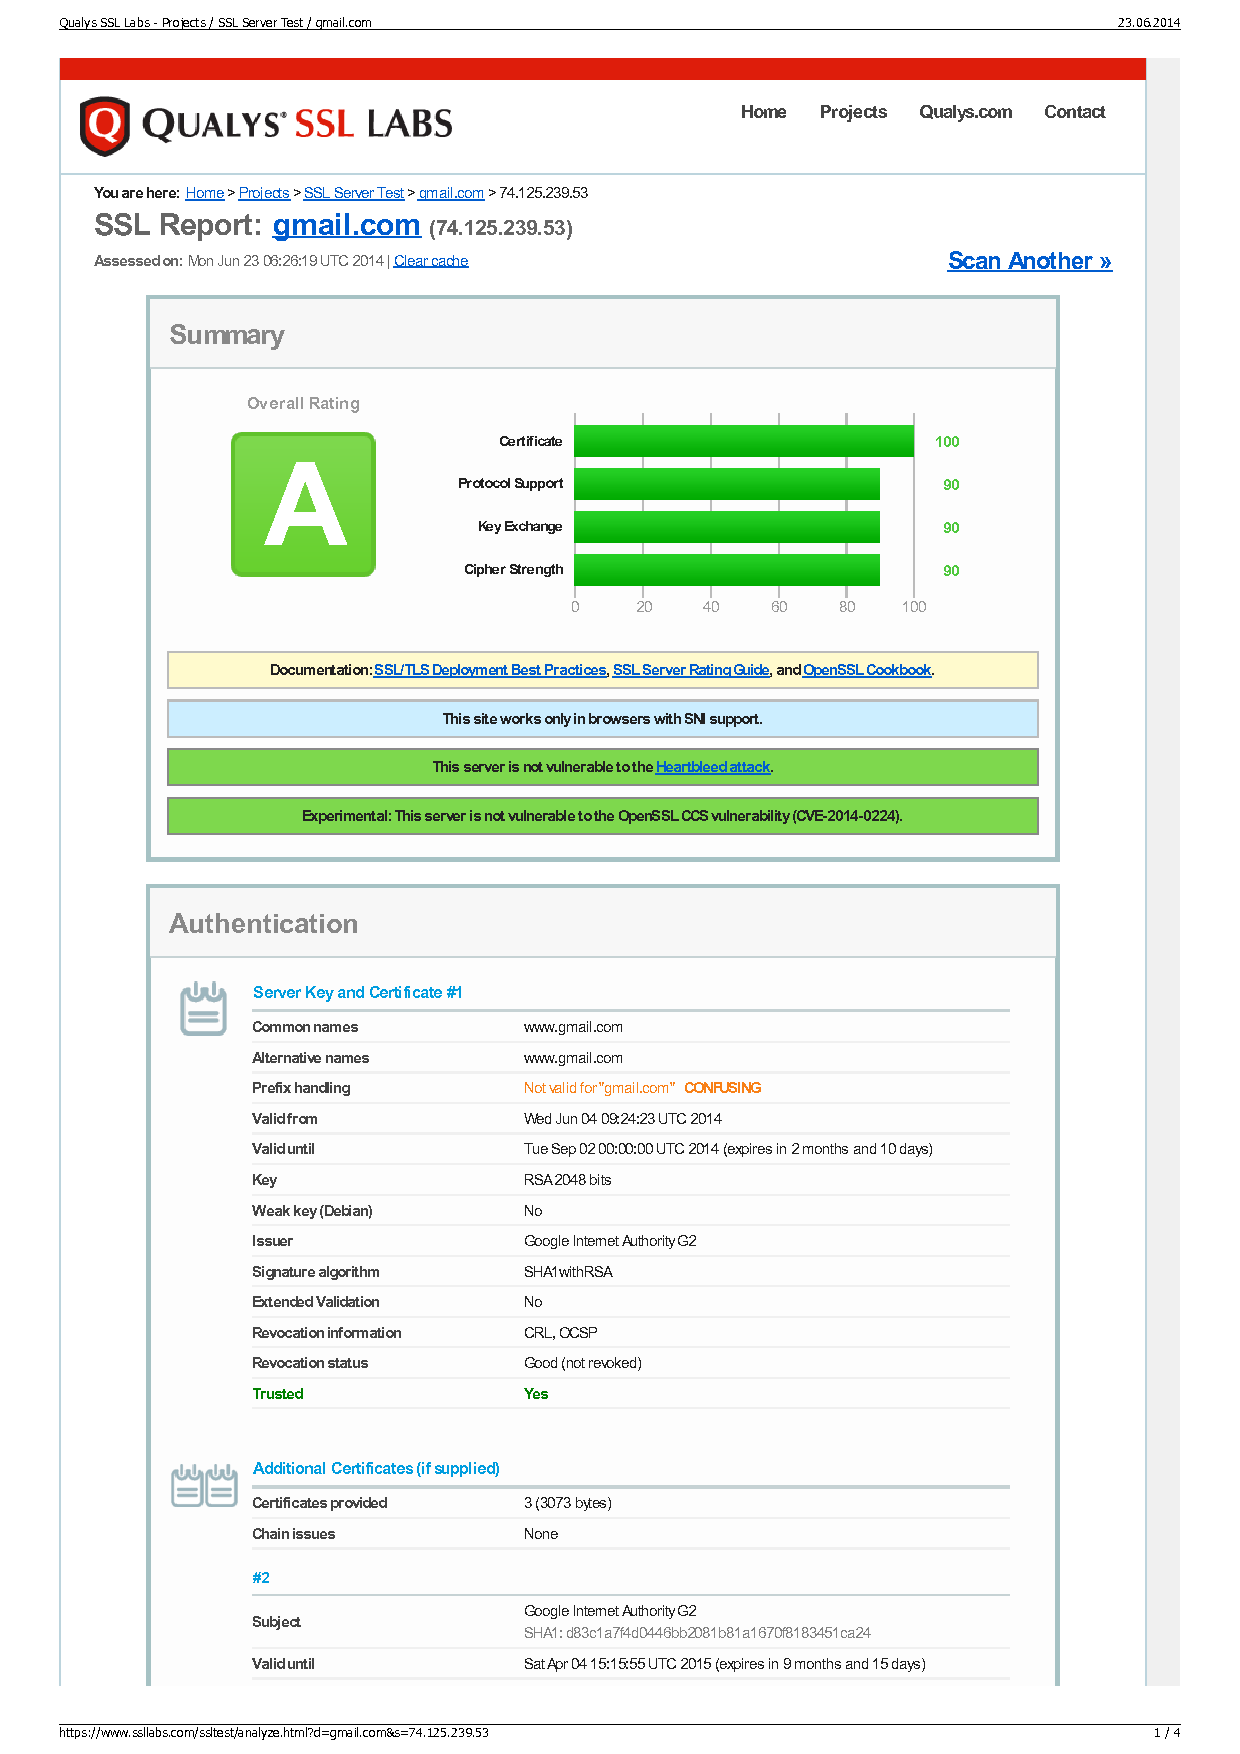
\includepdf[pages=1-4]{anlagen/SSLServerTest-gmail.pdf}
		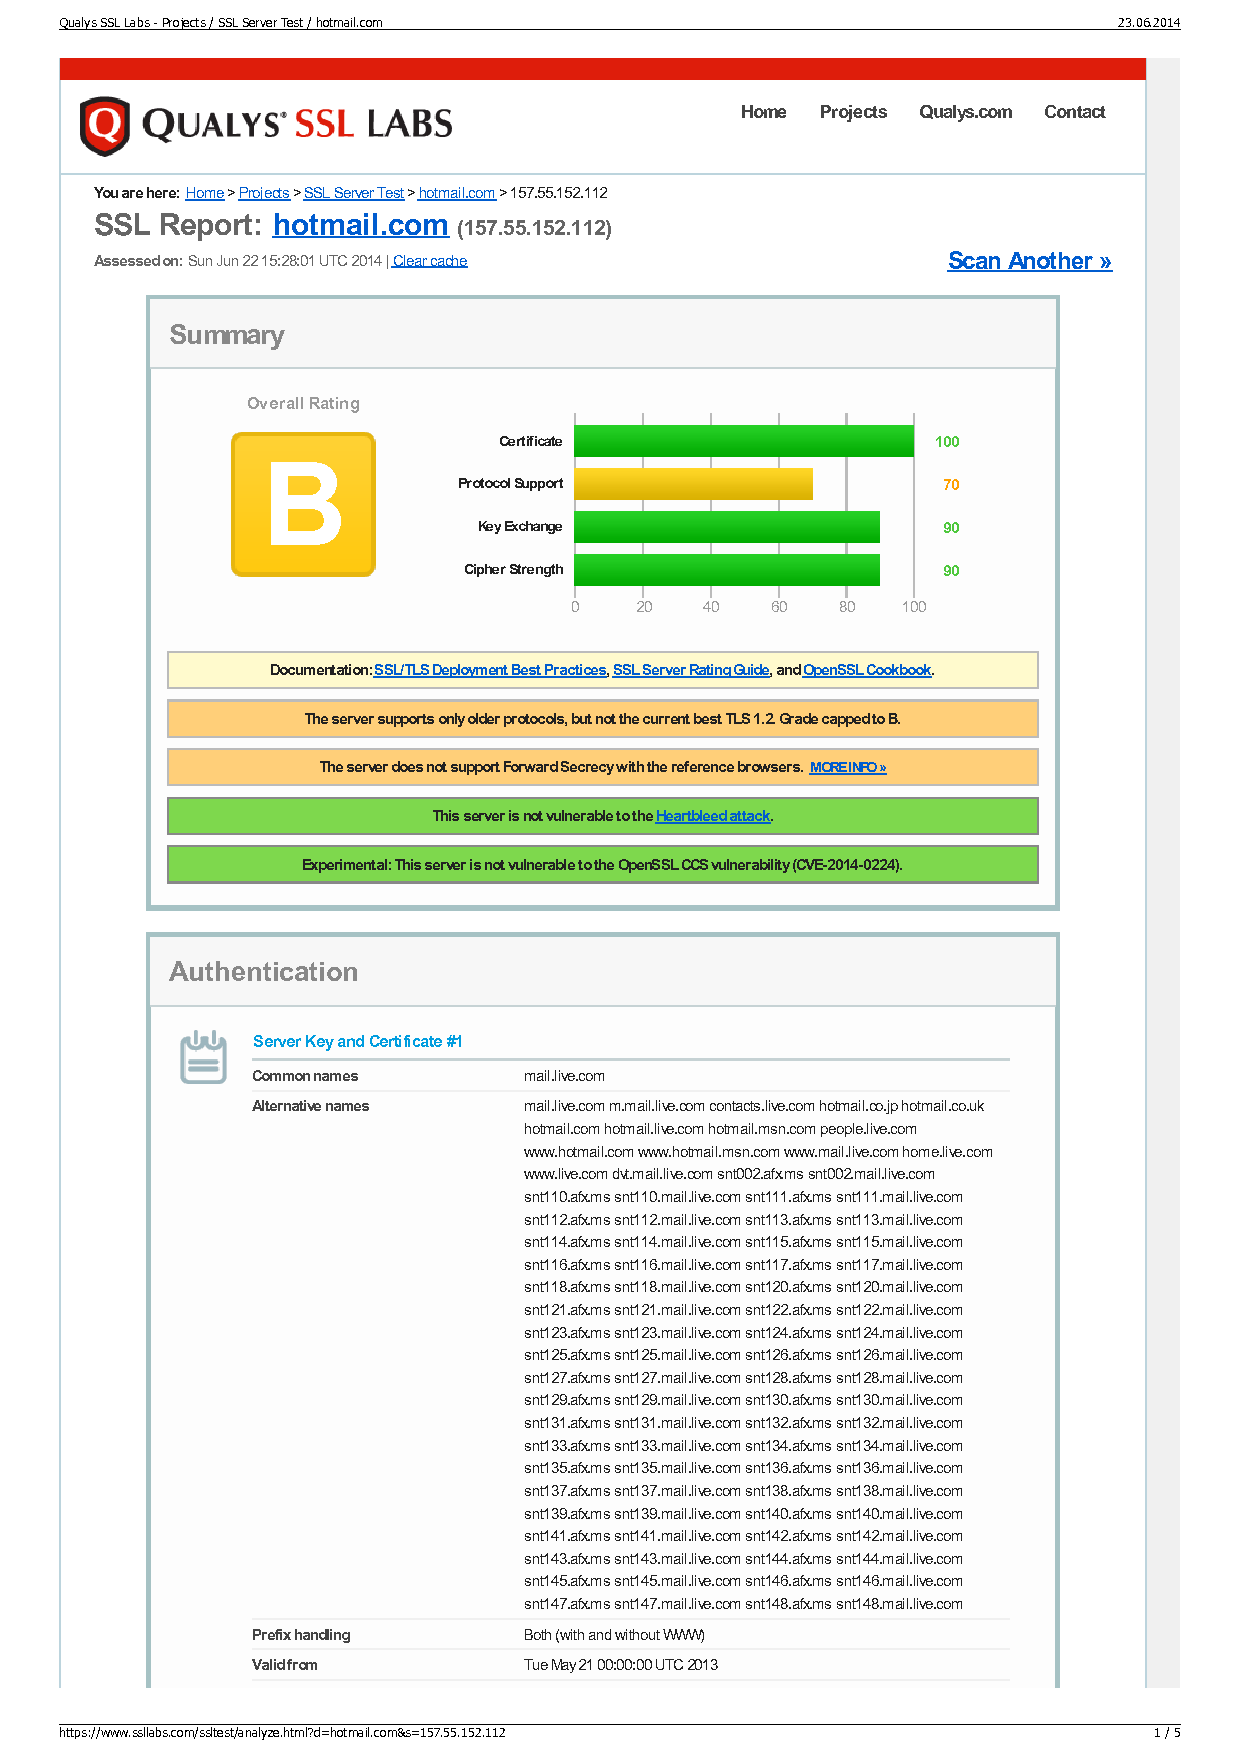
\includepdf[pages=1-5]{anlagen/SSLServerTest-hotmail.pdf}
		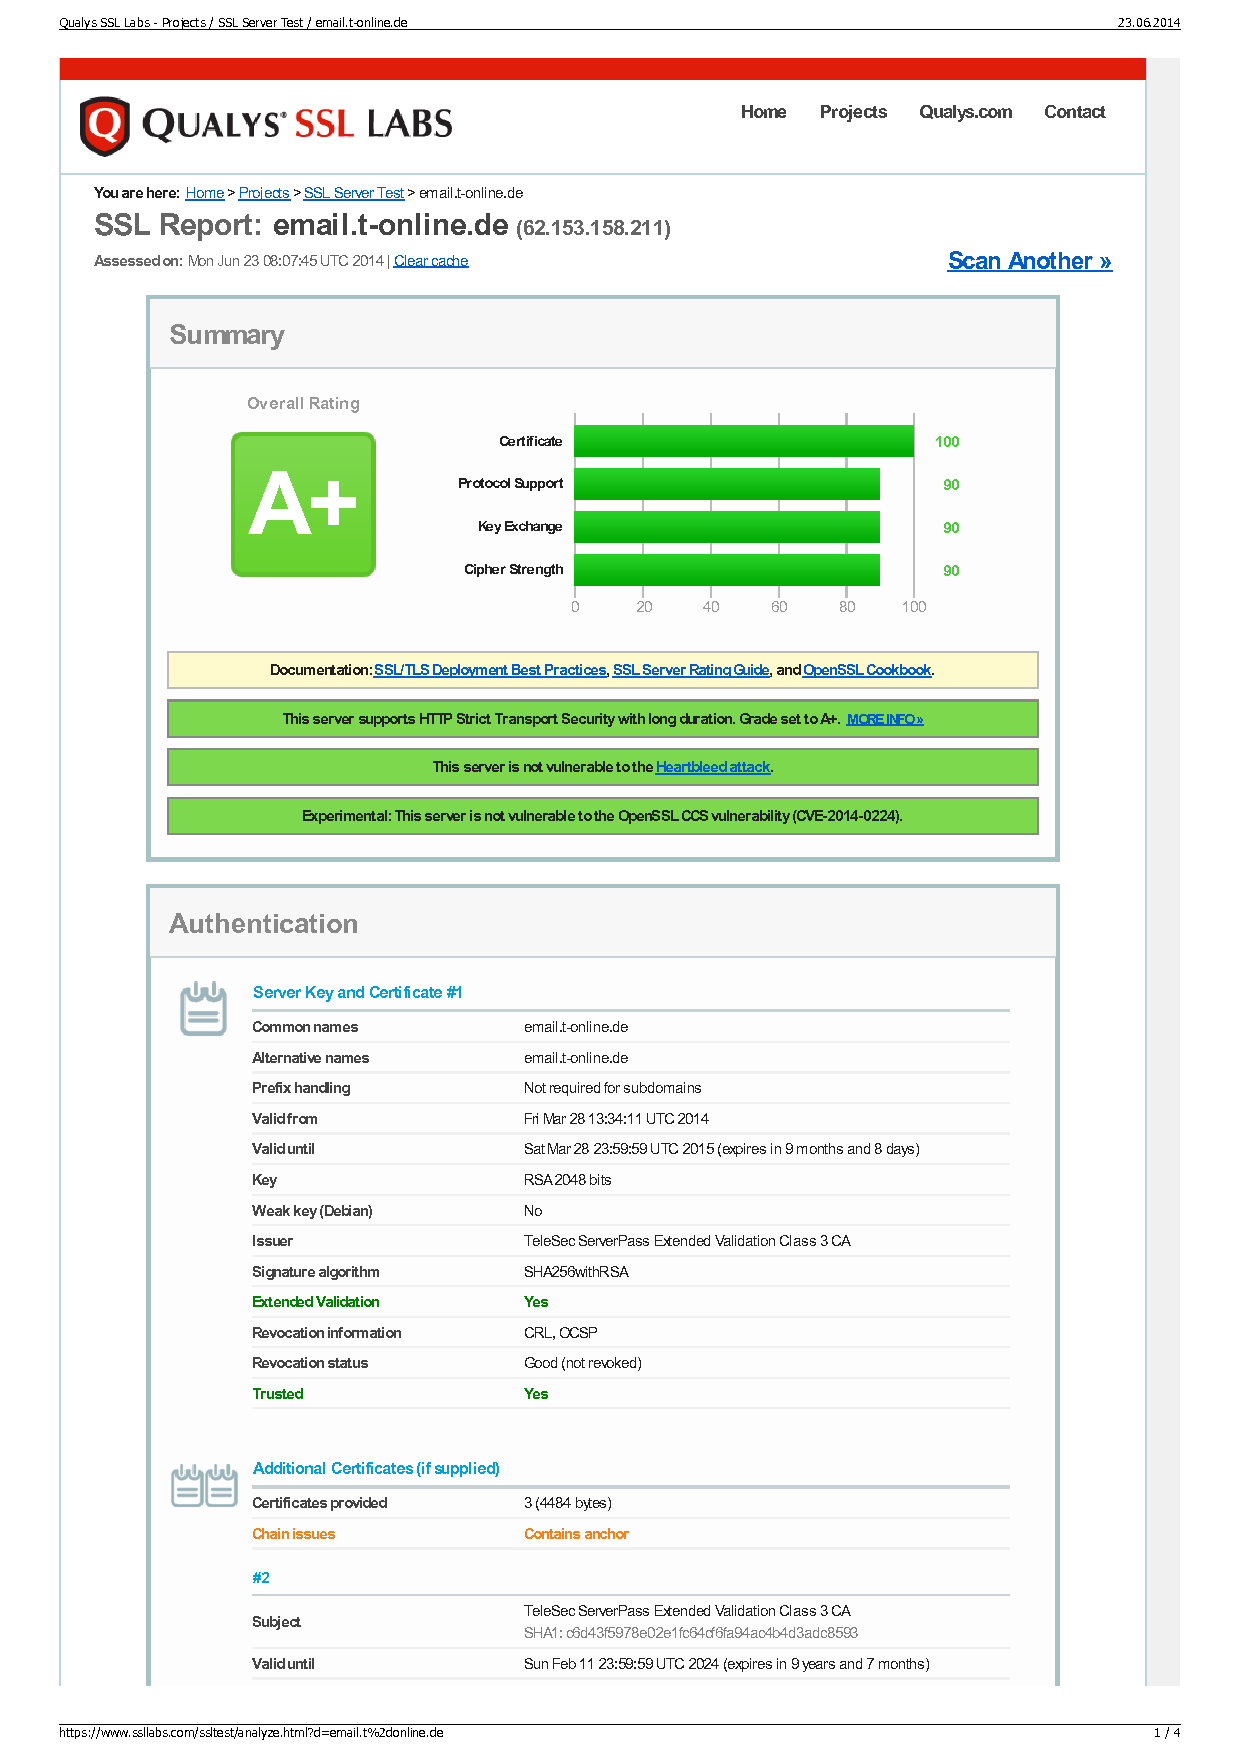
\includepdf[pages=1-4]{anlagen/SSLServerTest-t-online.pdf}
		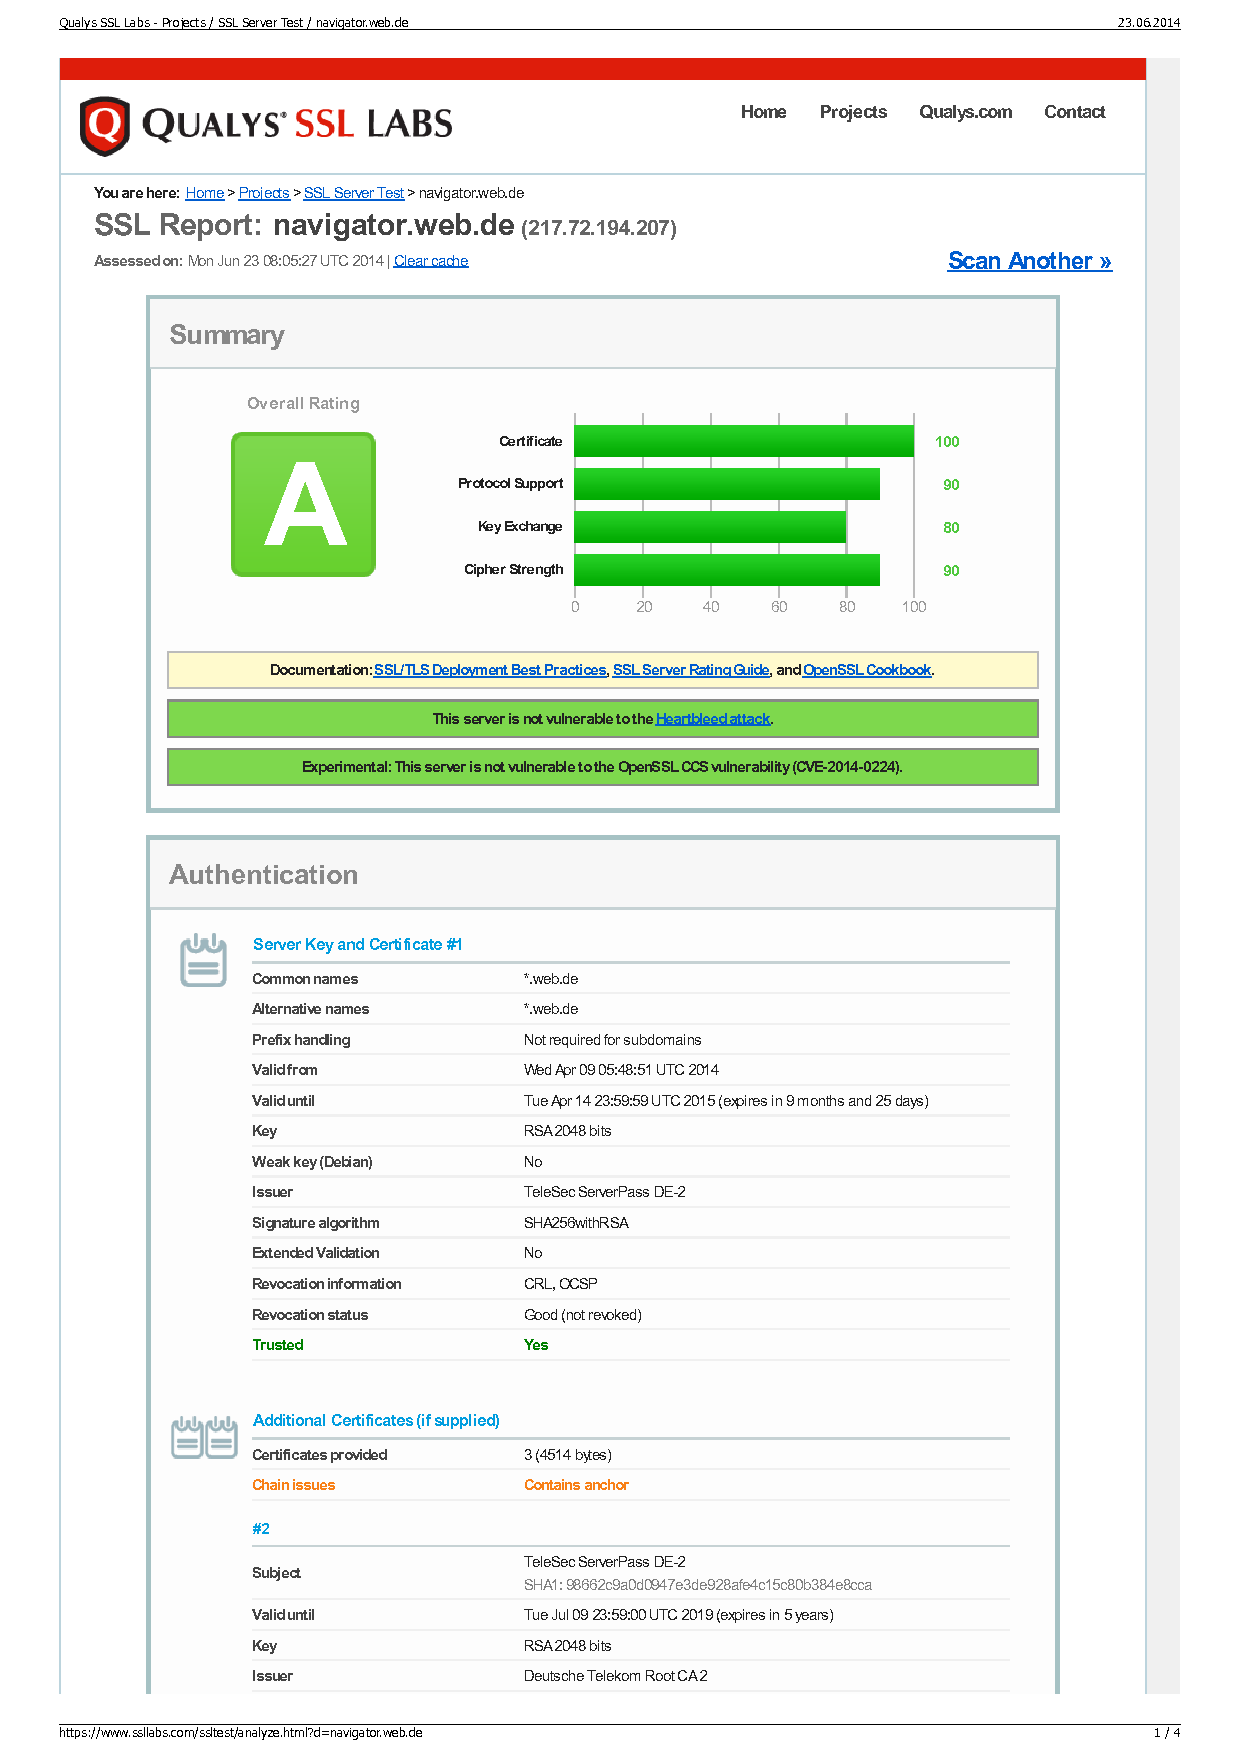
\includepdf[pages=1-4]{anlagen/SSLServerTest-web.pdf}
		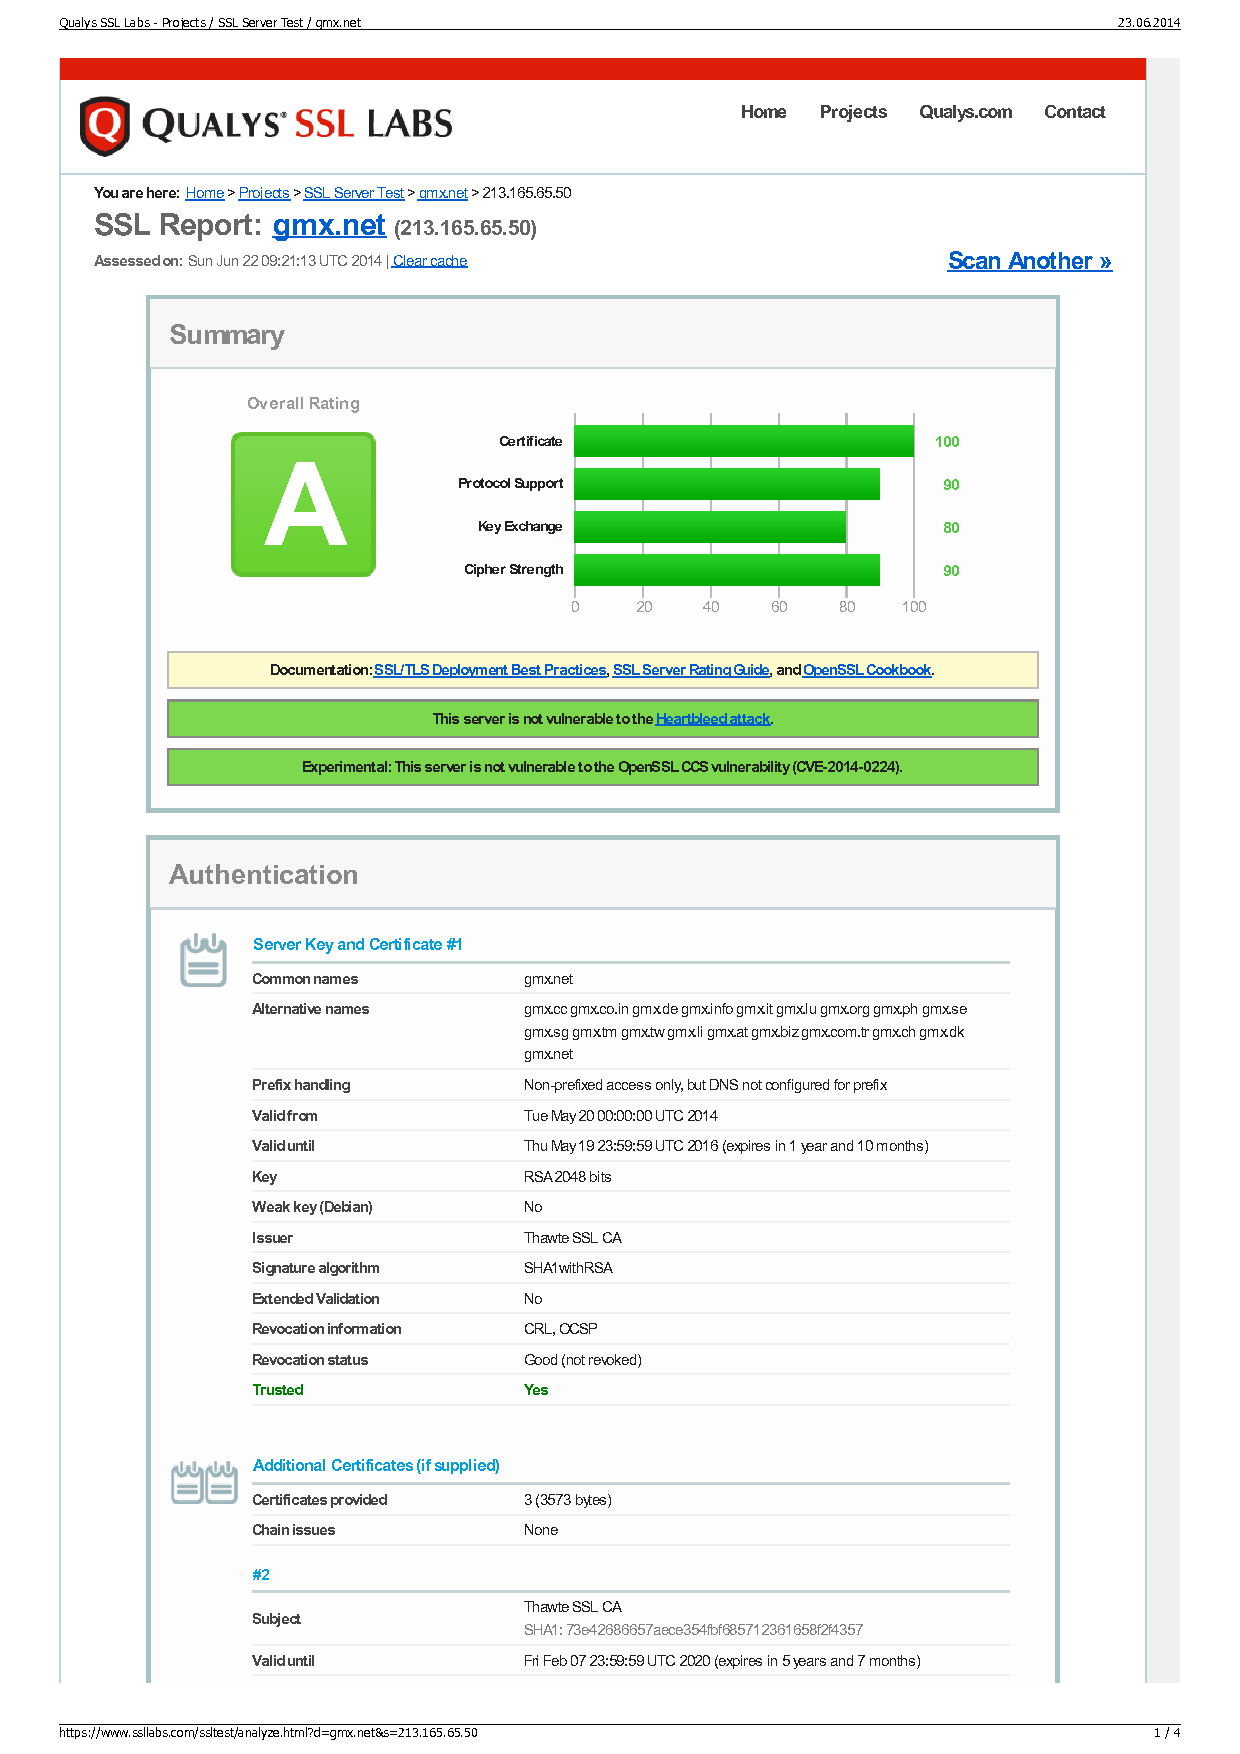
\includepdf[pages=1-4]{anlagen/SSLServerTest-gmx.pdf}
		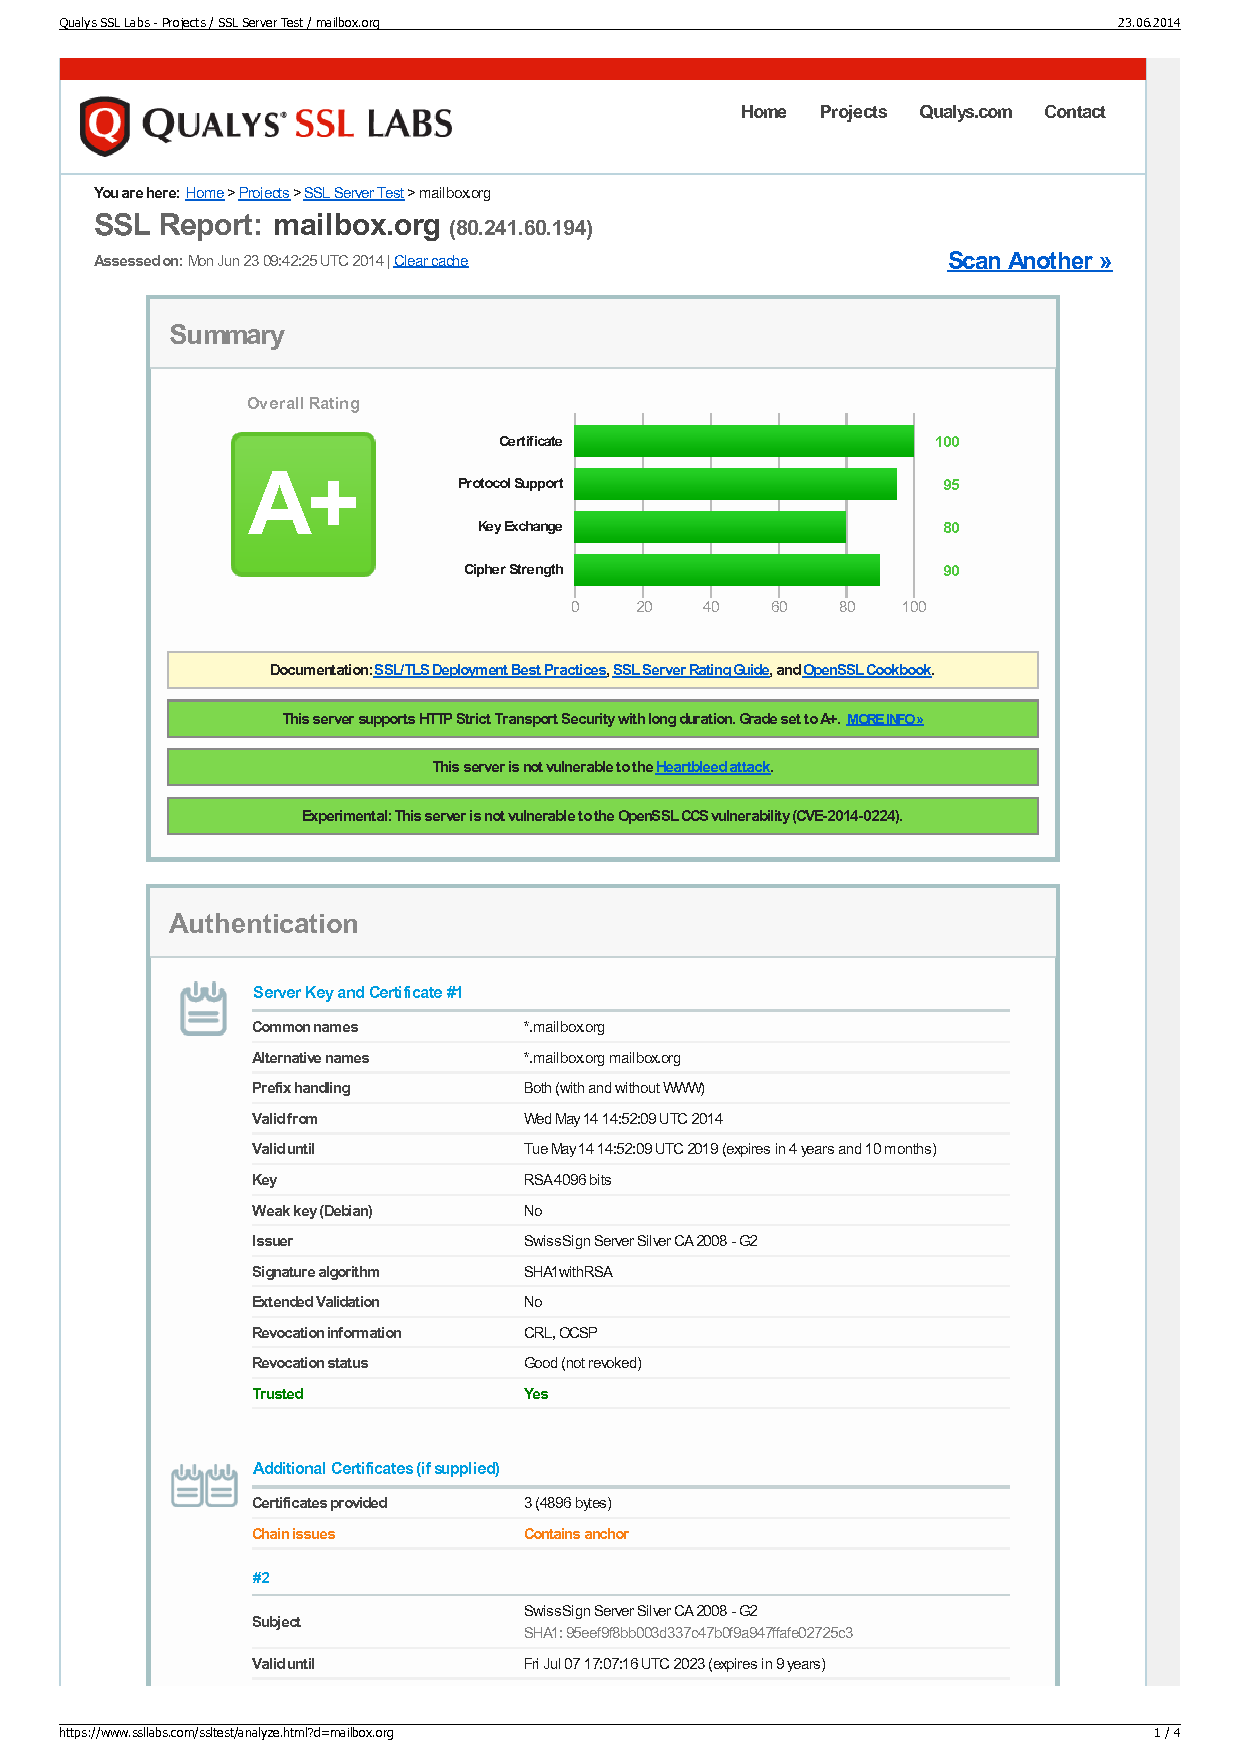
\includepdf[pages=1-4]{anlagen/SSLServerTest-mailbox.pdf}
		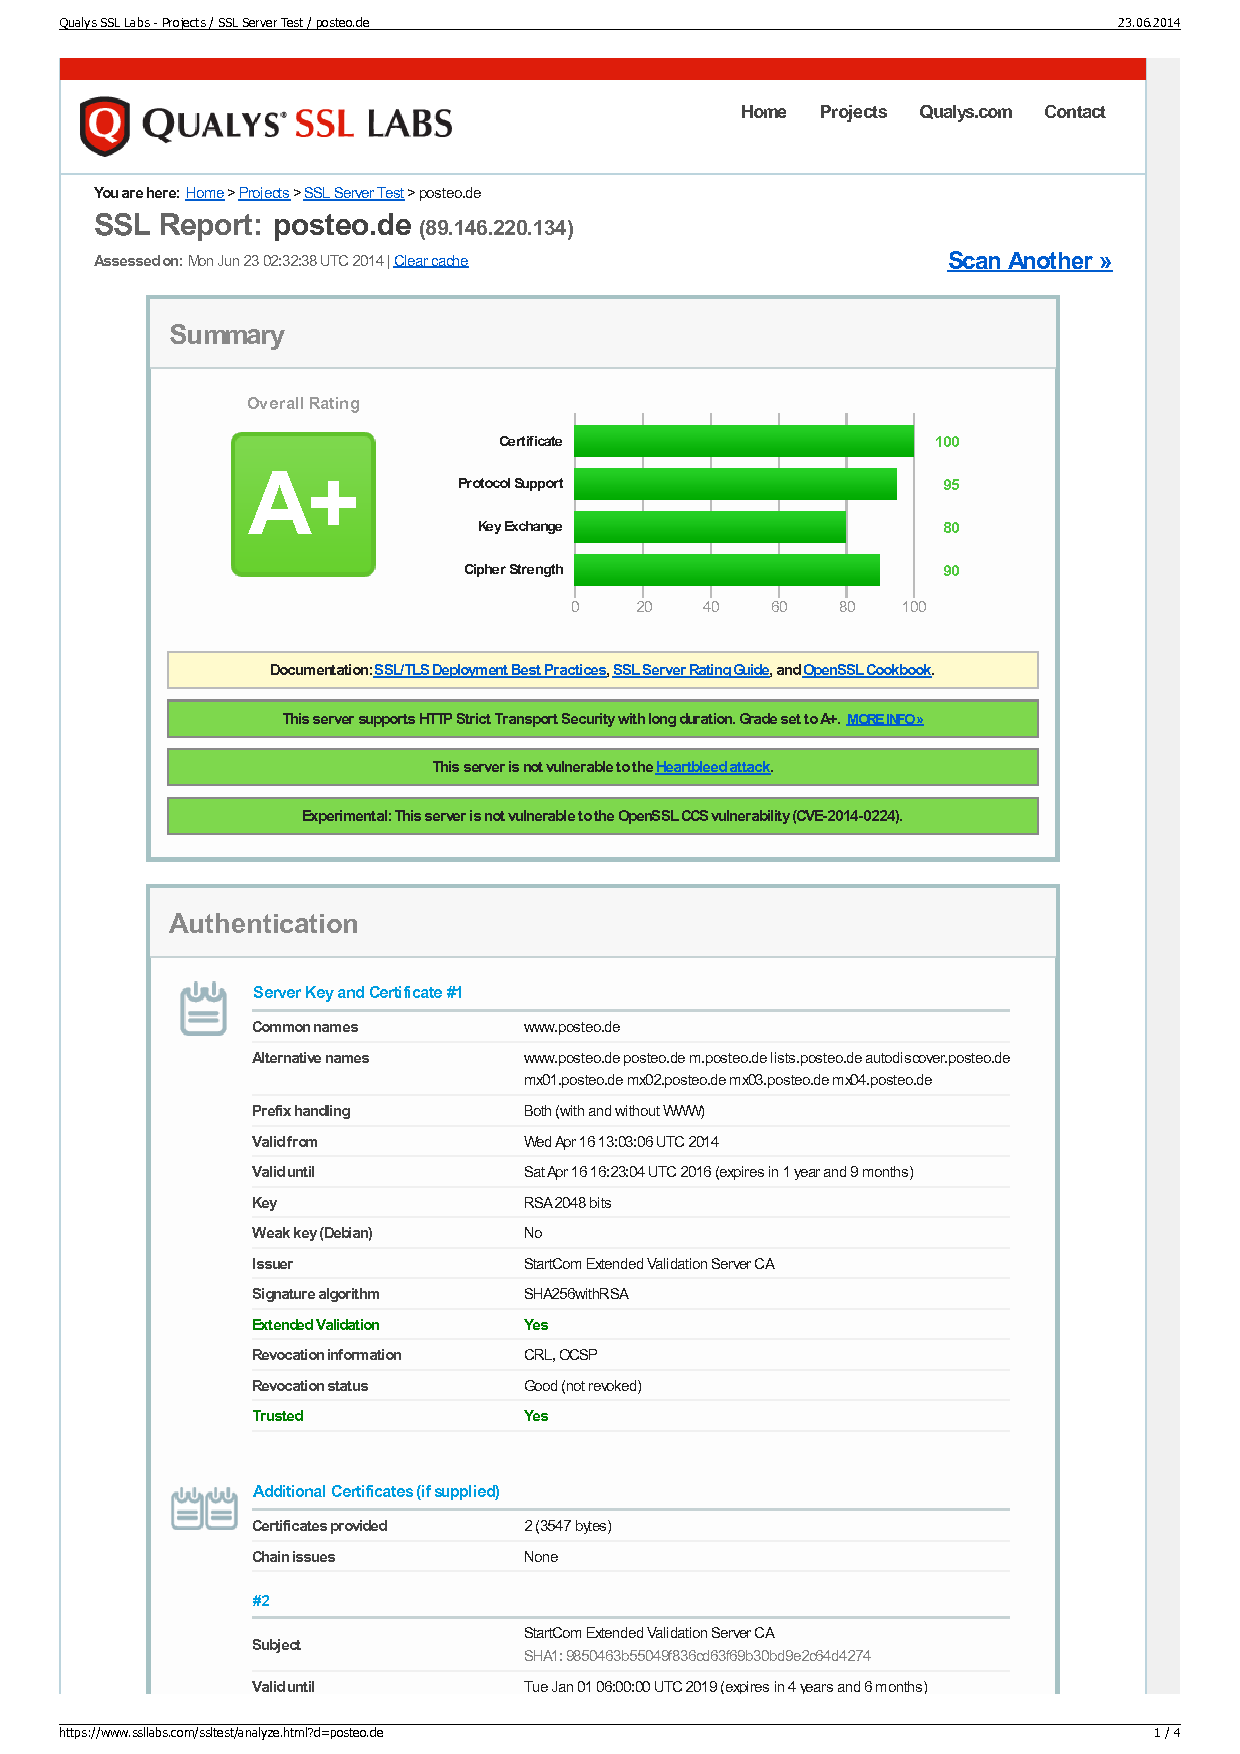
\includepdf[pages=1-4]{anlagen/SSLServerTest-posteo.pdf}
		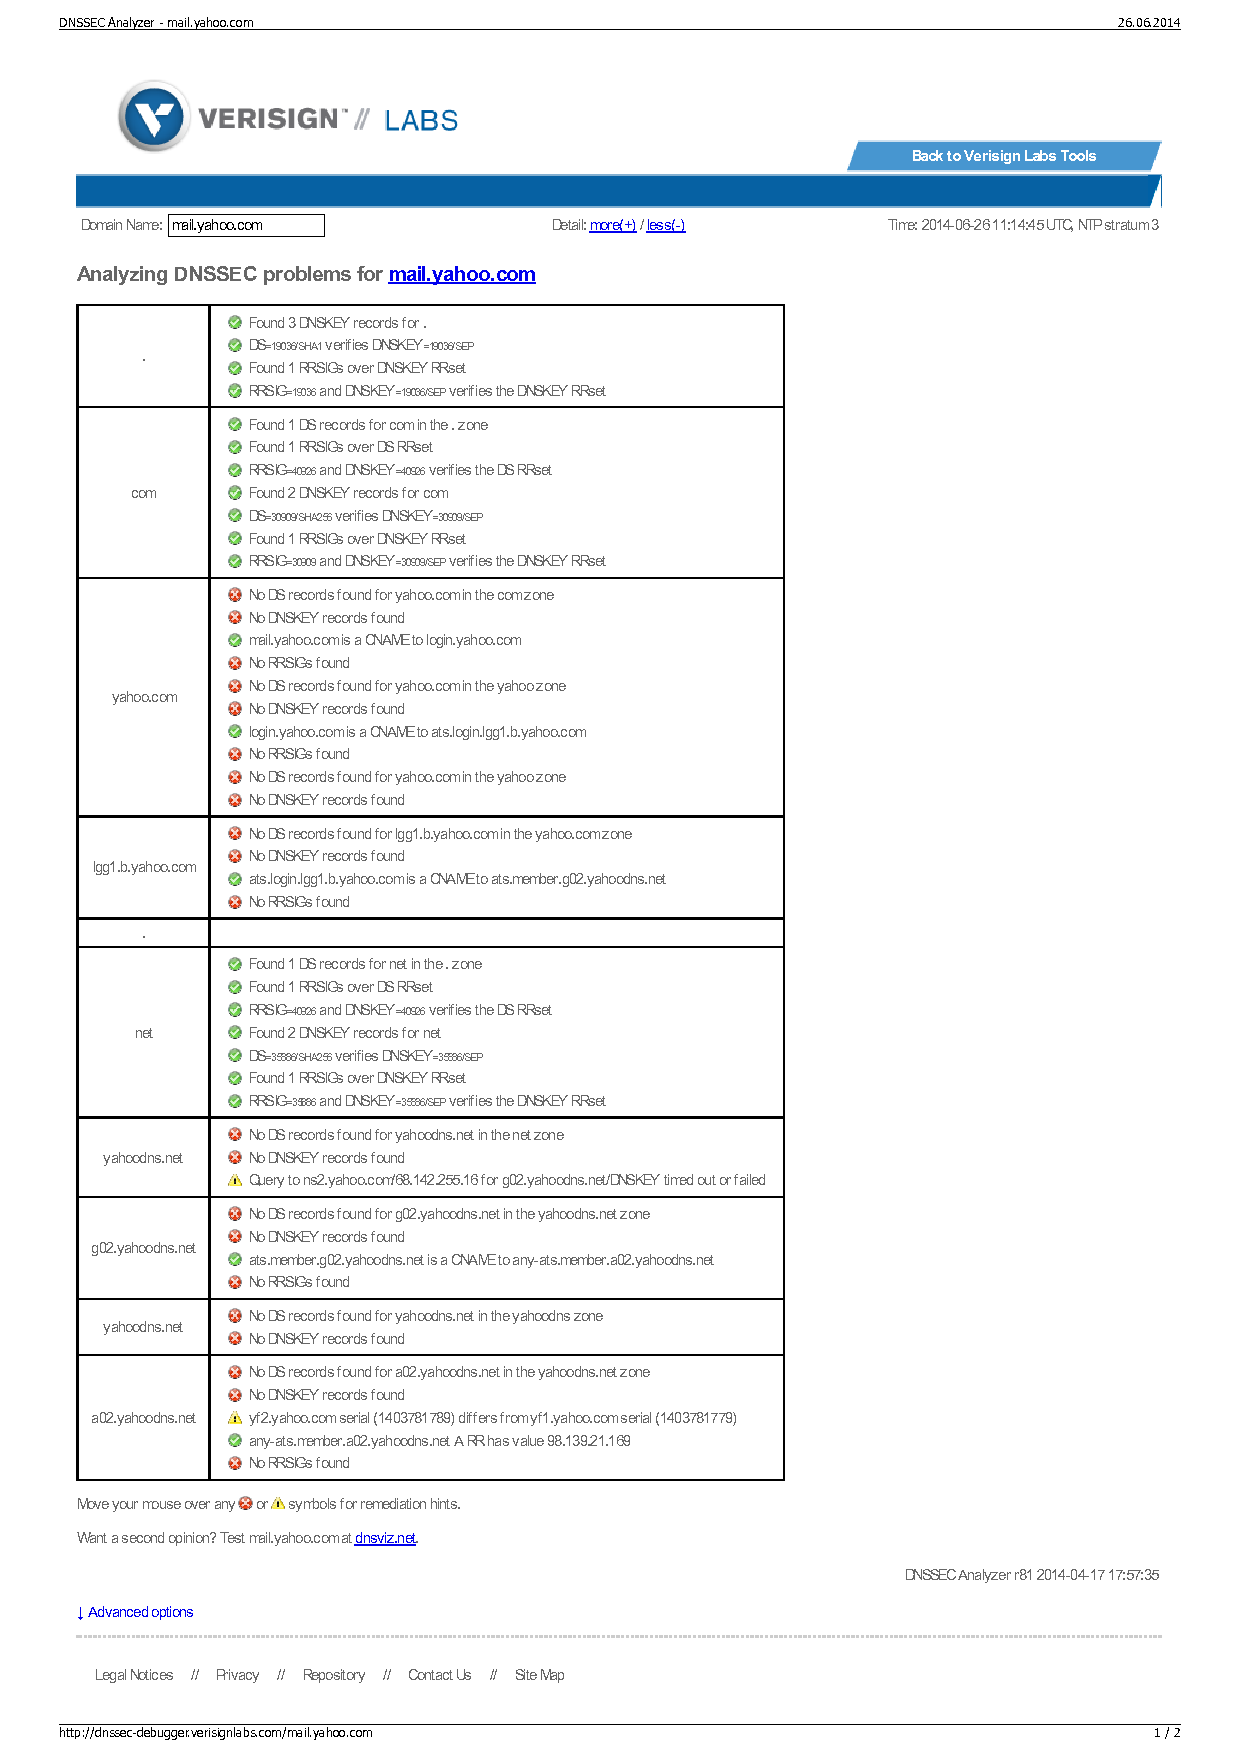
\includepdf[pages=1-2]{anlagen/DNSSECAnalyzer-yahoo.pdf}
		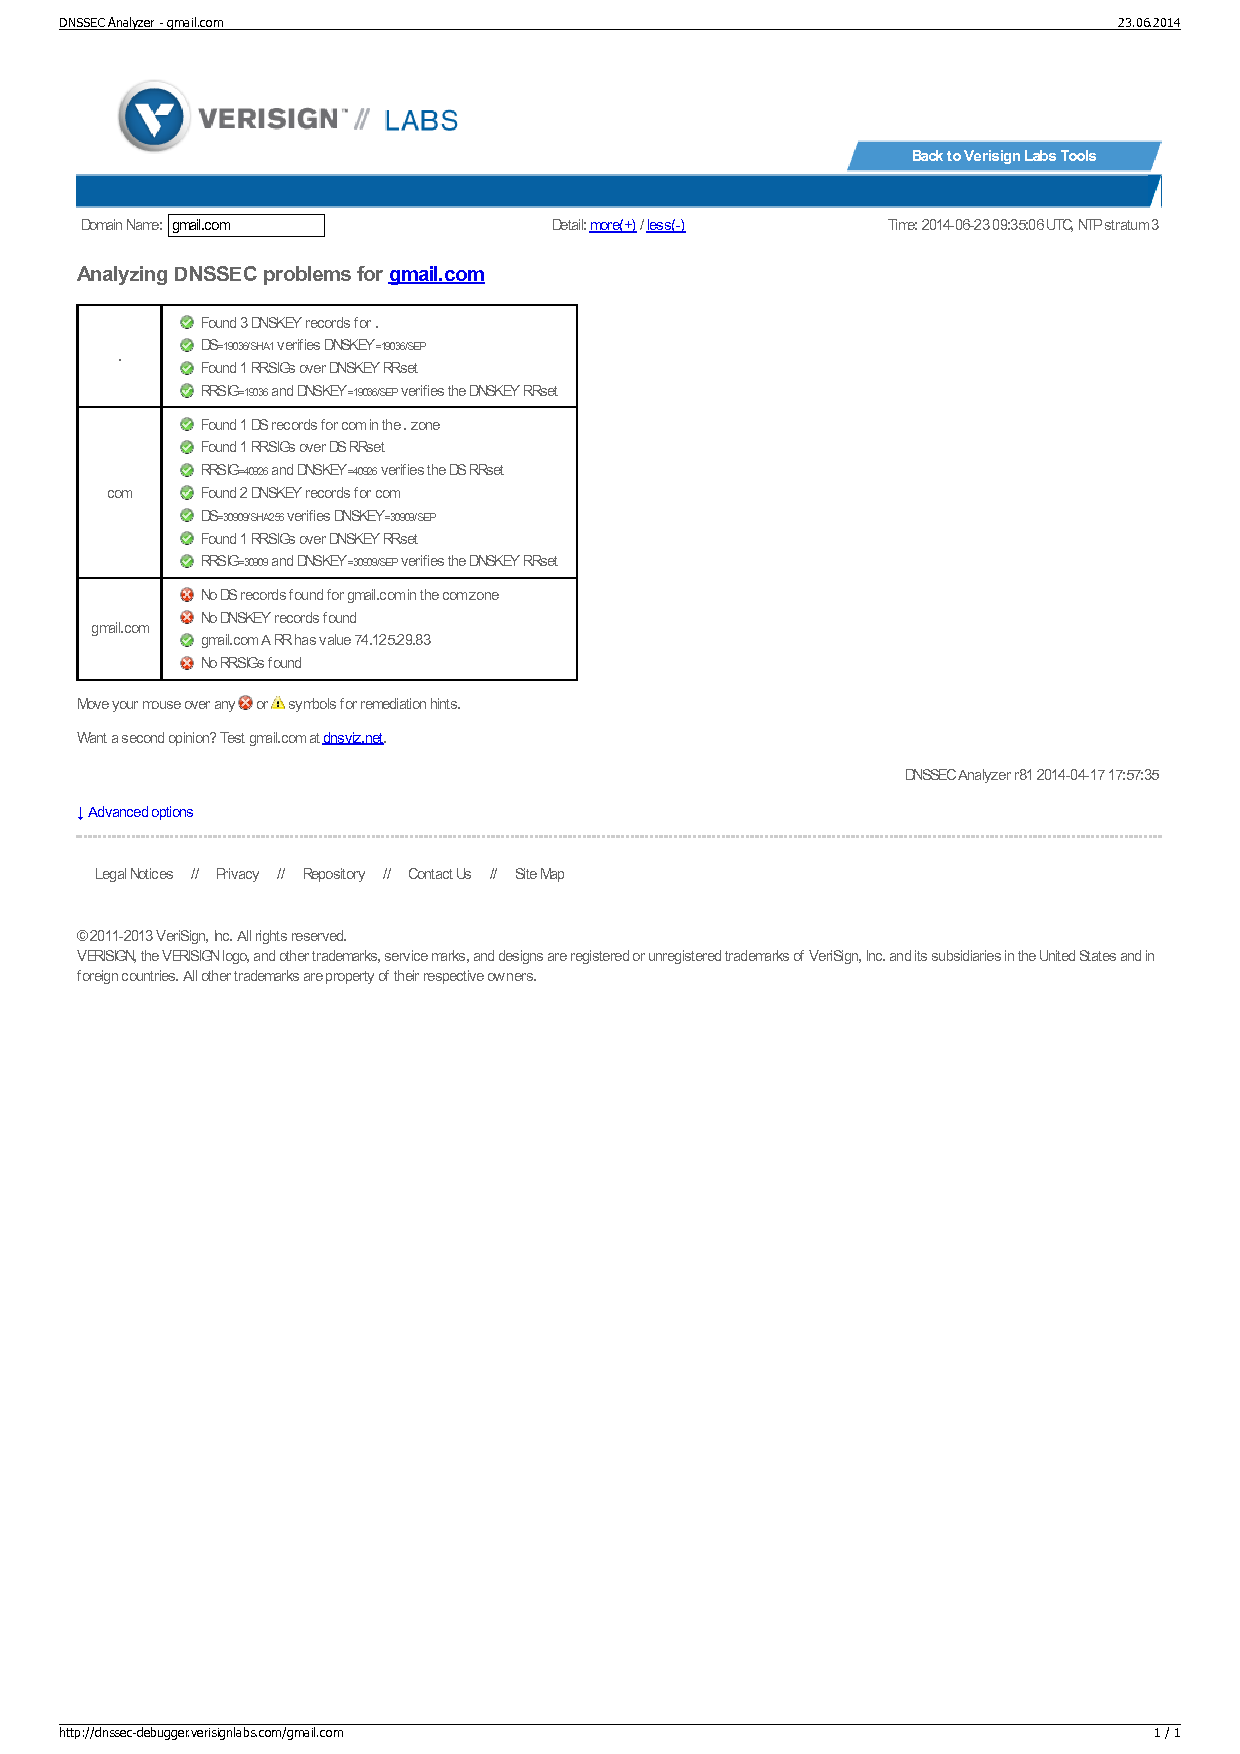
\includepdf[pages=1]{anlagen/DNSSECAnalyzer-gmail.pdf}
		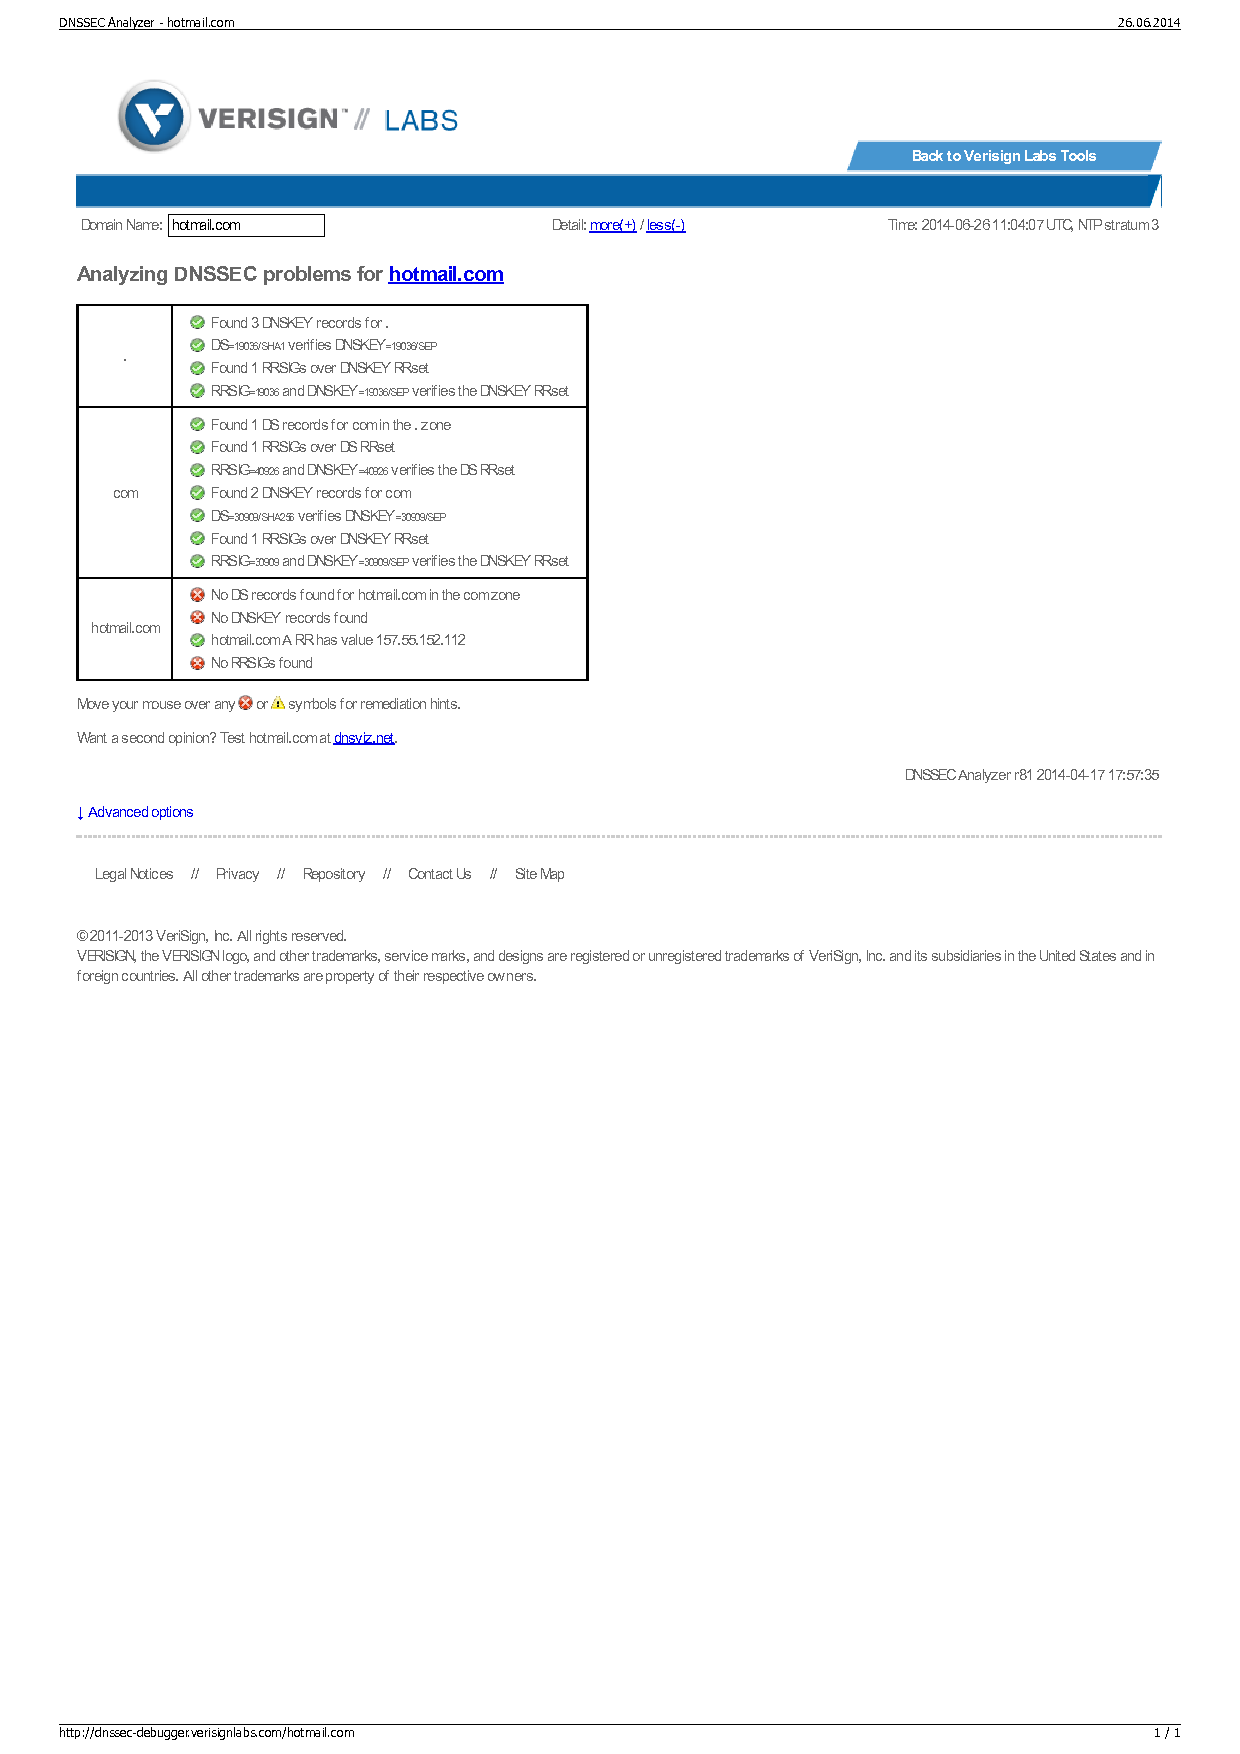
\includepdf[pages=1]{anlagen/DNSSECAnalyzer-hotmail.pdf}
		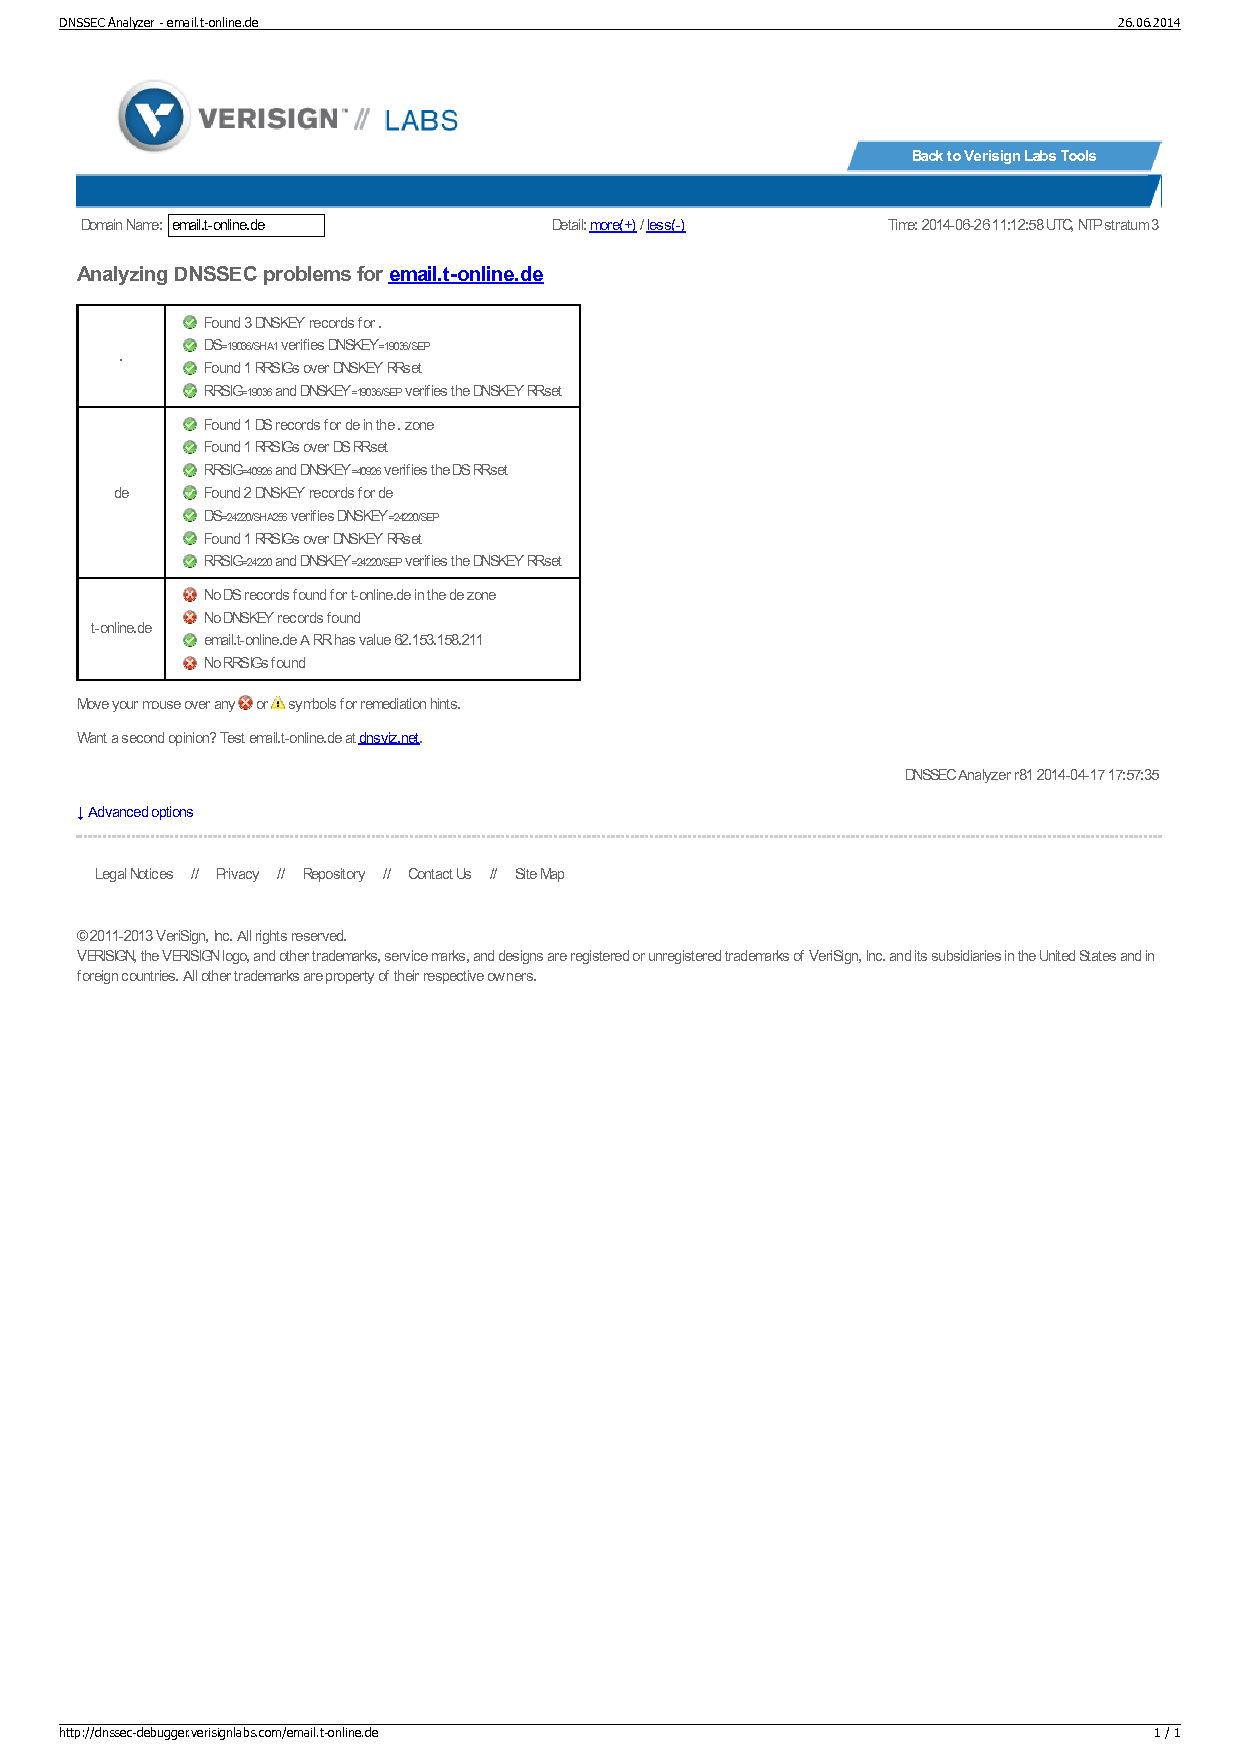
\includepdf[pages=1]{anlagen/DNSSECAnalyzer-t-online.pdf}
		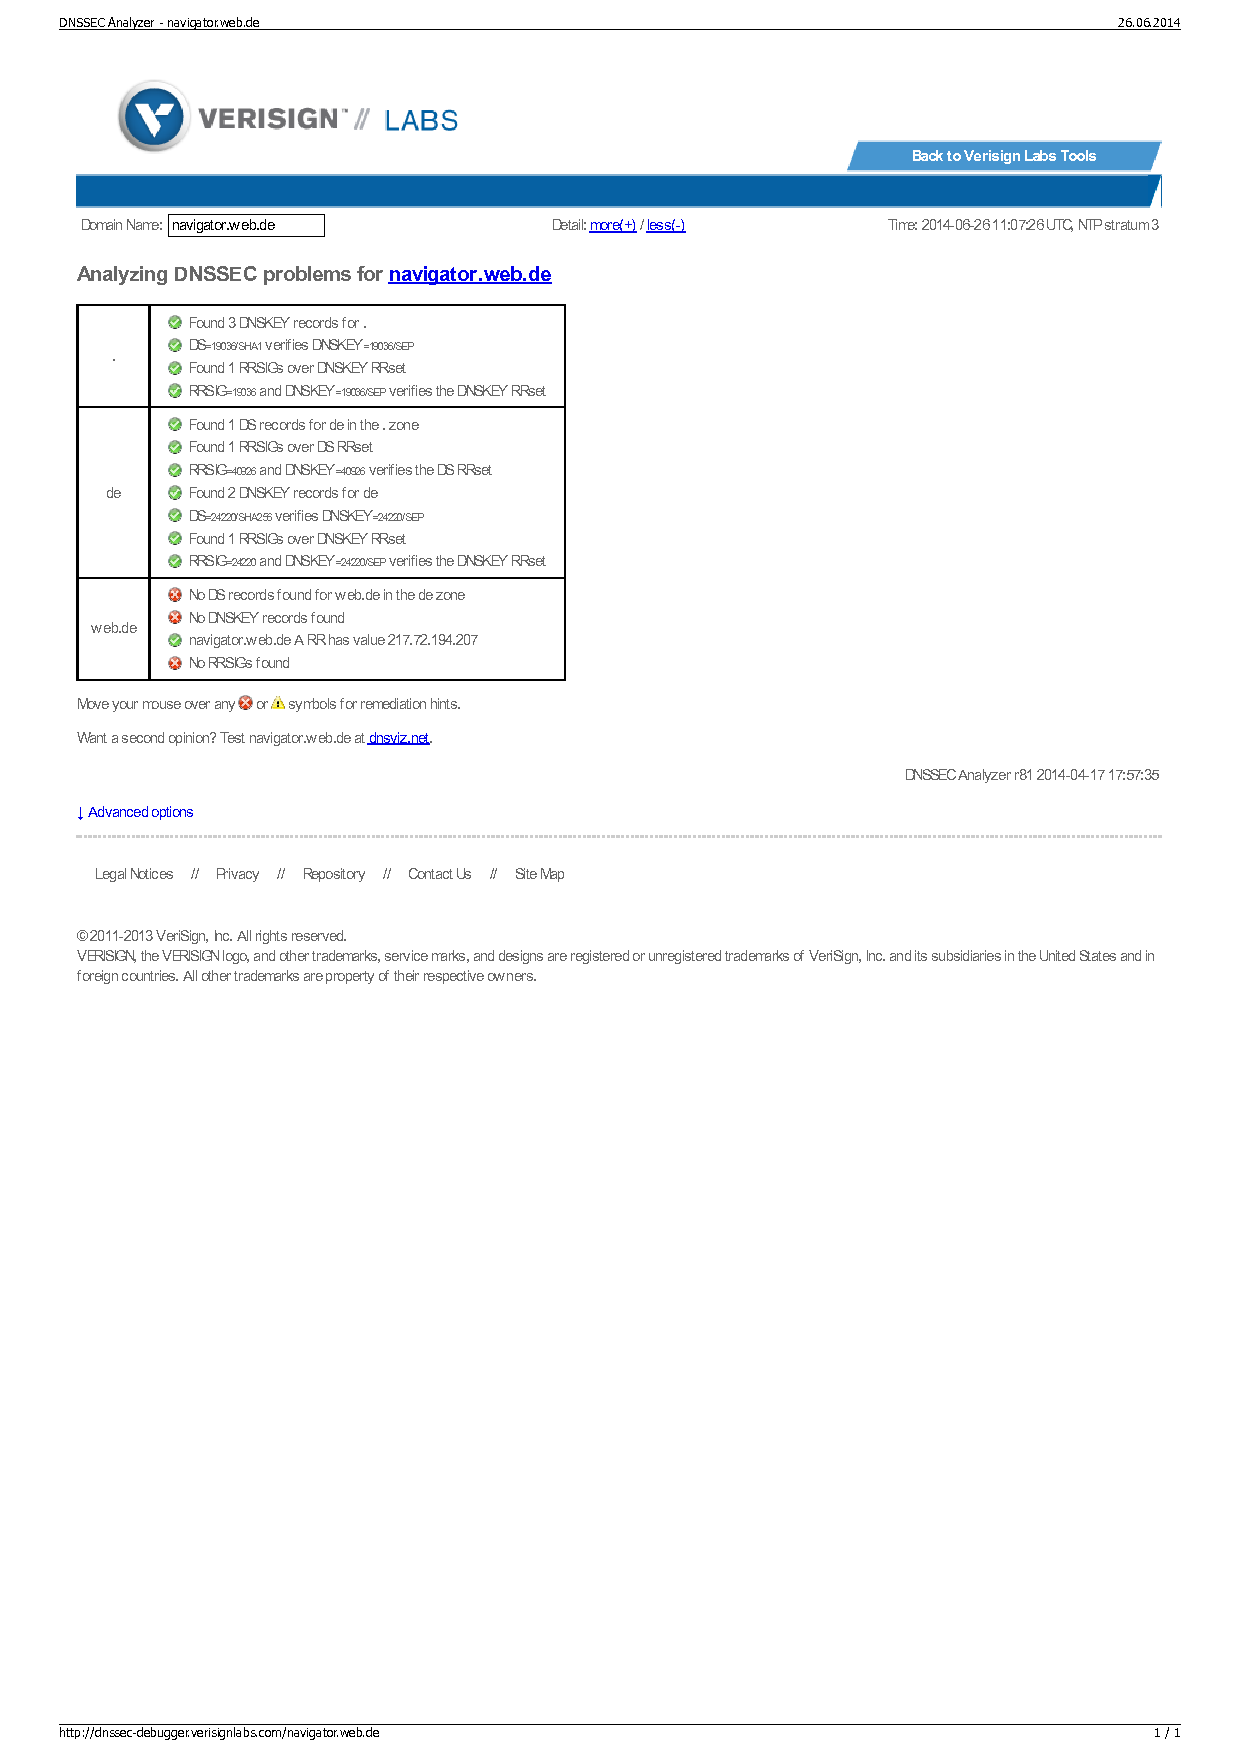
\includepdf[pages=1]{anlagen/DNSSECAnalyzer-web.pdf}
		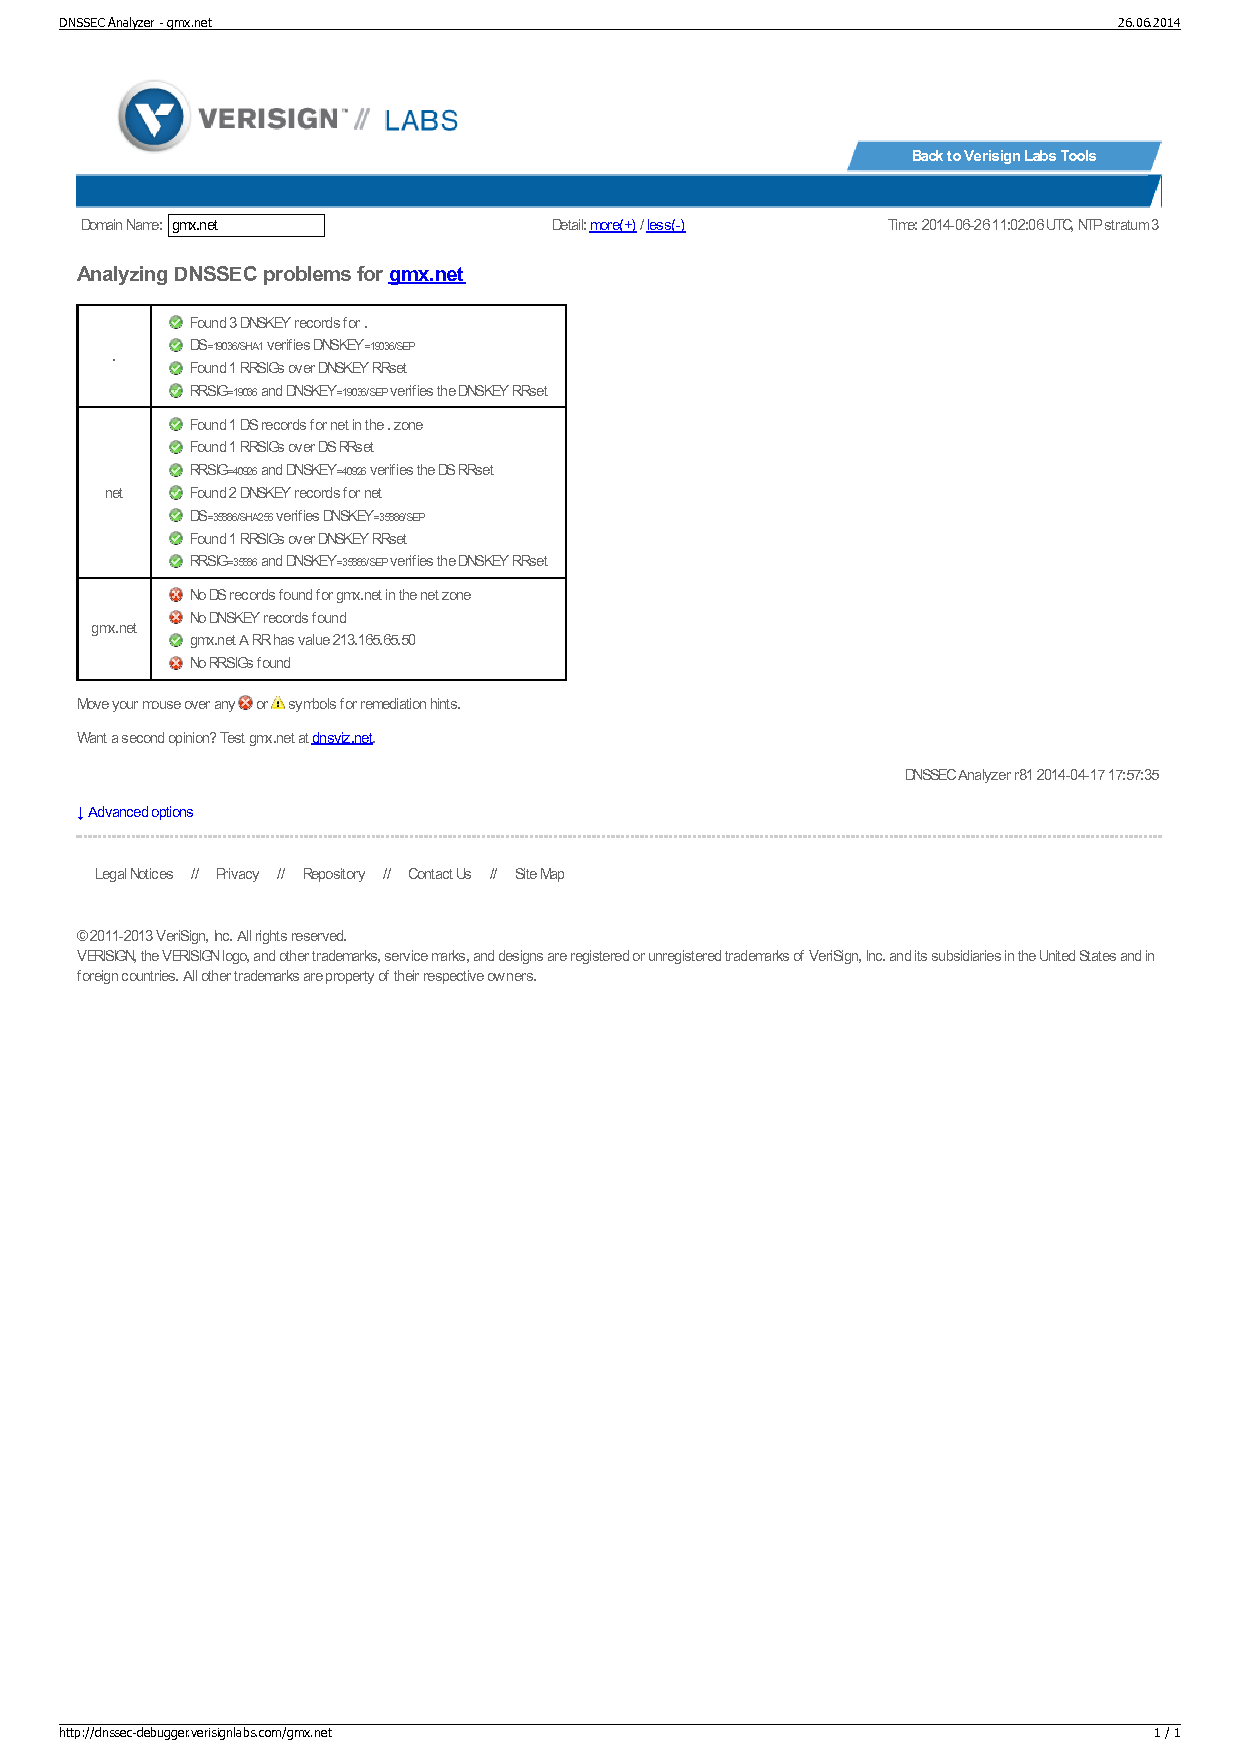
\includepdf[pages=1]{anlagen/DNSSECAnalyzer-gmx.pdf}
		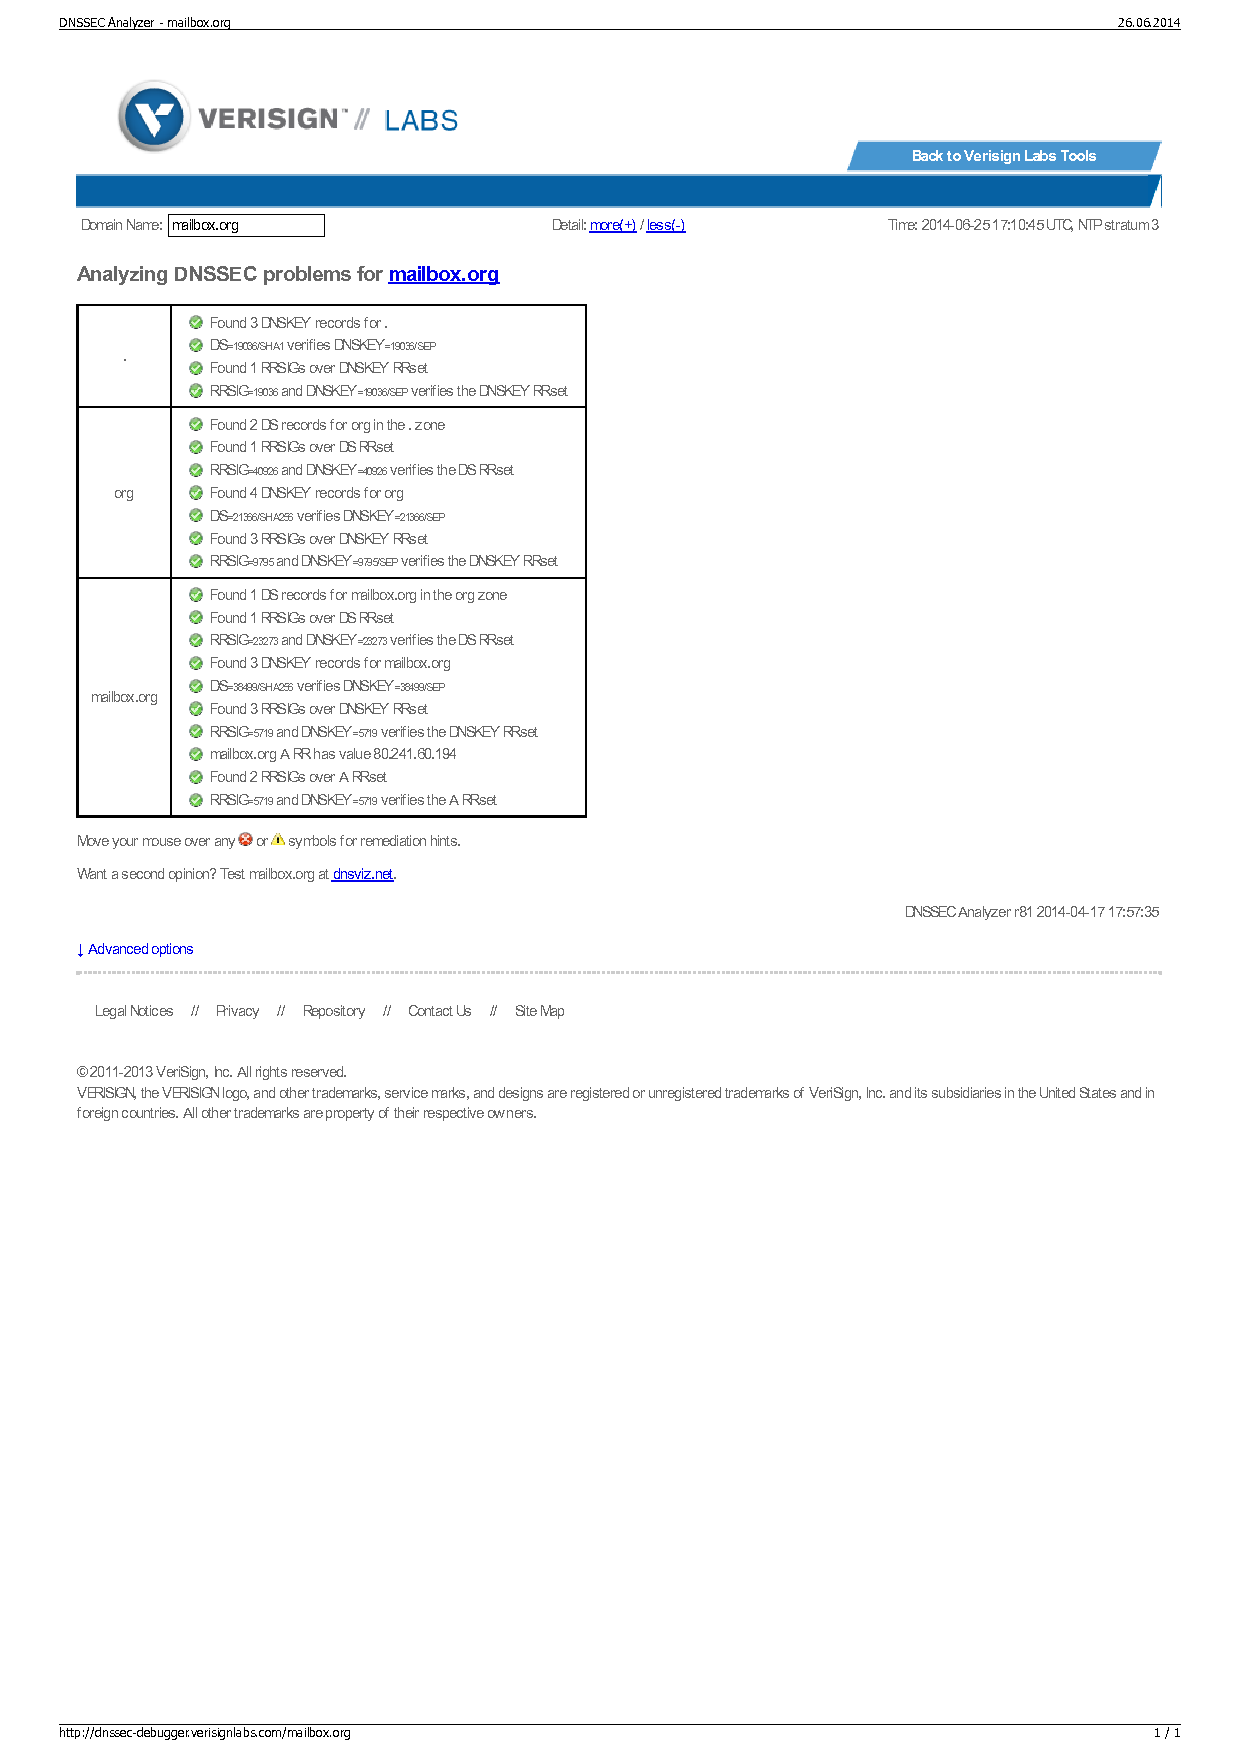
\includepdf[pages=1]{anlagen/DNSSECAnalyzer-mailbox.pdf}
		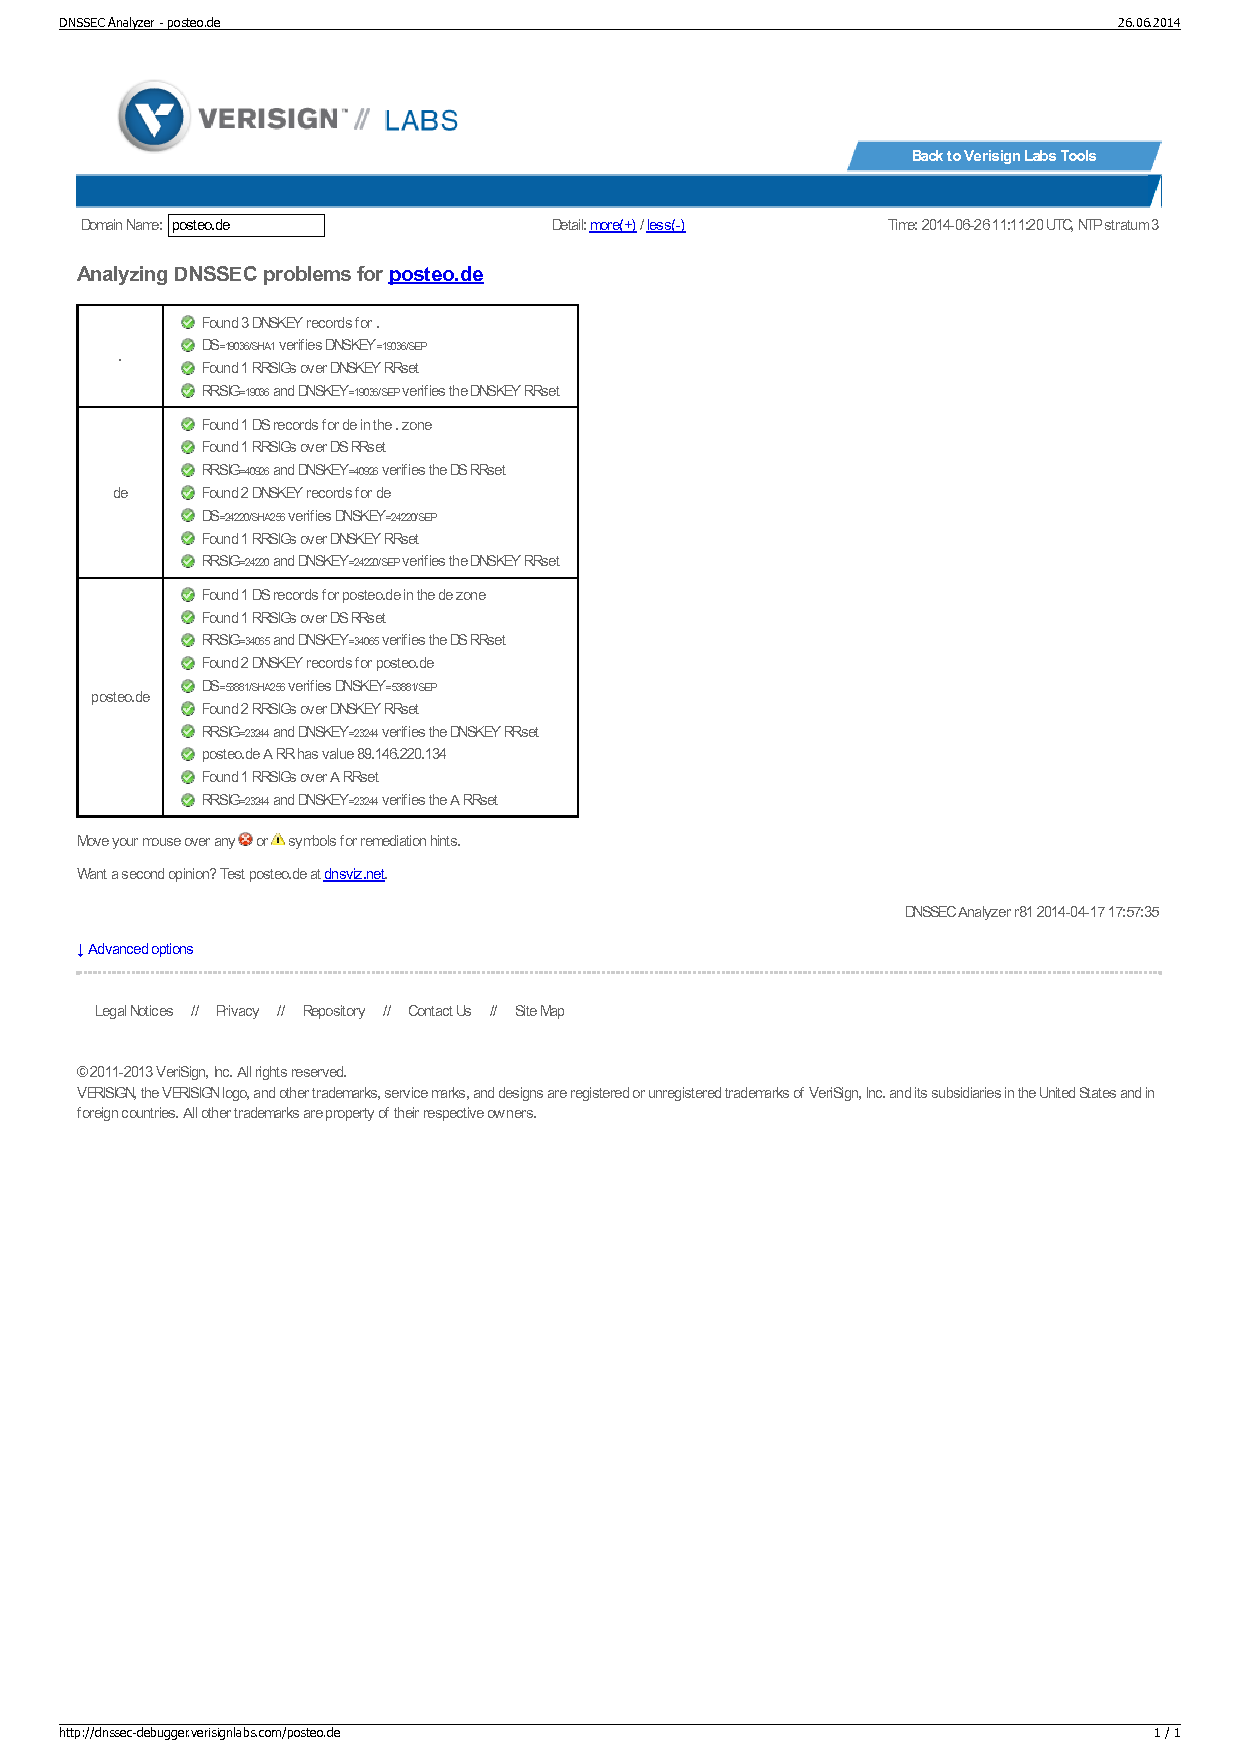
\includepdf[pages=1]{anlagen/DNSSECAnalyzer-posteo.pdf}
\end{document}